% ----------------------------------------------------------
% Resultados e Discussões (Gerado Automaticamente do Pipeline)
% ----------------------------------------------------------
\chapter{Resultados e Discussão}
\label{cap:resultados}

Este capítulo apresenta os resultados práticos obtidos a partir do pipeline de análise de telemetria de rede Wi-Fi, divididos em etapas que cobrem a validação de dados, análise descritiva, representações temporais, correlação linear, testes formais de hipótese e classificação operativa dos Access Points.

\section{Validação de Consistência dos Dados}

\subsection{Quantidade de Registros}

A tabela abaixo resume a quantidade de registros encontrados nos logs de telemetria antes e depois do processo de deduplicação (remoção de duplicados exatos).

\begin{table}[H]
\IBGEtab{%
  \caption{Quantidade de Registros}%
  \label{tab:data_validacao_de_dados_1}%
}{%
  \resizebox{\textwidth}{!}{%
    \begin{tabular}{lcccc}
      \toprule
      Fabricante & Registros Originais & Registros Duplicados Removidos & Registros Limpos & \% de Redundância \\
      \midrule
      \textbf{Ruckus} & 318.074 & 0 & 318.074 & 0,00\% \\
      \textbf{UniFi} & 36.180 & 0 & 36.180 & 0,00\% \\
      \bottomrule
    \end{tabular}%
  }%
}{%
  \fonte{Produzido pelos autores.}%
}
\end{table}

\textit{Nota: Registros duplicados ocorrem por sobreposição em polling repetido do coletor. A remoção evita viés nas análises estatísticas.}

\subsection{Período Coberto pela Coleta}

\begin{table}[H]
\IBGEtab{%
  \caption{Período Coberto pela Coleta}%
  \label{tab:data_validacao_de_dados_2}%
}{%
  \resizebox{\textwidth}{!}{%
    \begin{tabular}{lccc}
      \toprule
      Fabricante & Data/Hora Inicial (Min) & Data/Hora Final (Max) & Duração Efetiva \\
      \midrule
      \textbf{Ruckus} & 23/06/2026 00:00 & 10/07/2026 23:55 & 17 days 23:55:00 \\
      \textbf{UniFi} & 23/06/2026 00:02 & 10/07/2026 23:57 & 17 days 23:55:00 \\
      \bottomrule
    \end{tabular}%
  }%
}{%
  \fonte{Produzido pelos autores.}%
}
\end{table}

\textit{Nota: Ambos os datasets cobrem o mesmo período temporal (de 23/06/2026 00:00 a 10/07/2026 23:55), garantindo que os cenários de carga de rede sejam diretamente comparáveis.}

\subsection{Dados Ausentes (Missing Values)}

O percentual de dados nulos ou ausentes para cada variável após a limpeza:

\begin{table}[H]
\IBGEtab{%
  \caption{Dados Ausentes (Missing Values)}%
  \label{tab:data_validacao_de_dados_3}%
}{%
  \resizebox{\textwidth}{!}{%
    \begin{tabular}{lccc}
      \toprule
      Coluna Padronizada & \% Nulos Ruckus & \% Nulos UniFi & Tipo de Dado \\
      \midrule
      \texttt{timestamp} & 0,00\% & 0,00\% & Datetime \\
      \texttt{AP} & 0,00\% & 0,00\% & Categórico \\
      \texttt{cliente (MAC)} & 0,00\% & 0,00\% & Categórico \\
      \texttt{RSSI} & 10,34\% & 0,00\% & Numérico \\
      \texttt{signal} & 10,34\% & 0,00\% & Numérico \\
      \texttt{noise} & 10,34\% & 0,00\% & Numérico \\
      \texttt{canal} & 0,00\% & 0,00\% & Categórico \\
      \texttt{throughput\_tx\_mbps} & 0,00\% & 0,00\% & Numérico \\
      \texttt{throughput\_rx\_mbps} & 0,00\% & 0,00\% & Numérico \\
      \texttt{link\_speed\_tx\_mbps} & 6,51\% & 0,00\% & Numérico \\
      \texttt{link\_speed\_rx\_mbps} & 100,00\% & 0,00\% & Numérico \\
      \texttt{retransmissoes\_pct} & 0,00\% & 0,00\% & Numérico \\
      \texttt{volume\_tx\_mb} & 0,00\% & 0,00\% & Numérico \\
      \texttt{volume\_rx\_mb} & 0,00\% & 0,00\% & Numérico \\
      \texttt{padrão} & 0,00\% & 0,00\% & Categórico \\
      \bottomrule
    \end{tabular}%
  }%
}{%
  \fonte{Produzido pelos autores.}%
}
\end{table}

\subsection{Tratamento de Valores Nulos}

\begin{itemize}
  \item \textbf{Link Speed no Ruckus}: A taxa de modulação física de TX (\texttt{link\_speed\_tx\_mbps}) foi extraída com sucesso a partir do campo \texttt{throughput\_rate} (em Kbps) nos logs de telemetria da controladora SmartZone. A taxa RX correspondente (\texttt{link\_speed\_rx\_mbps}) não é informada nos logs brutos e é mantida como \texttt{NaN}.
  \item \textbf{Ruído (Noise) e Sinal (Signal) em Ruckus}: Alguns registros continham valores de sinal zerados ou vazios. Onde o sinal era -100 (vazio padrão) e SNR era 0, o ruído foi definido como NaN para evitar distorções de cálculo.
  \item \textbf{Valores Nulos na UniFi}: O dataset UniFi apresenta consistência total (0\% de nulos nas métricas principais de telemetria).

\end{itemize}
\subsection{Padronização das Unidades de Medida}

As colunas foram padronizadas da seguinte forma:
\begin{enumerate}
  \item \textbf{Sinal e Ruído}: Potência medida em \textbf{dBm}.
  \item \textbf{RSSI/SNR}: Medido em \textbf{dB} (ou índice relativo na UniFi).
  \item \textbf{Throughput}: Convertido em \textbf{Mbps} (Megabits por segundo) para Downstream (\texttt{tx}) e Upstream (\texttt{rx}).
  \item \textbf{Volume de Dados}: Convertido em \textbf{MB} (Megabytes) acumulados por cliente no período de observação.
  \item \textbf{Retransmissões}: Medidas em porcentagem (\textbf{\%}) de pacotes retransmitidos.
  \item \textbf{Link Speed}: Modulação de velocidade física convertida em \textbf{Mbps}.

\end{enumerate}
\subsection{Equivalência de Métricas (Mapeamento Ruckus vs UniFi)}

A tabela abaixo mostra a relação entre os campos extraídos de cada fabricante que representam as mesmas grandezas físicas:

\begin{table}[H]
\IBGEtab{%
  \caption{Equivalência de Métricas (Mapeamento Ruckus vs UniFi)}%
  \label{tab:data_validacao_de_dados_4}%
}{%
  \resizebox{\textwidth}{!}{%
    \begin{tabular}{lccc}
      \toprule
      Grandeza Física & Métrica Ruckus (Raw) & Métrica UniFi (Raw) & Coluna Padronizada Final \\
      \midrule
      Potência do Sinal & \texttt{signal\_rssi} & \texttt{signal} & \texttt{signal} (dBm) \\
      Relação Sinal/Ruído & \texttt{snr} & \texttt{rssi} & \texttt{RSSI} (dB) \\
      Throughput Downstream & \texttt{tx\_bytes / uptime} & \texttt{tx\_bytes\_r \textsuperscript{*} 8} & \texttt{throughput\_tx\_mbps} \\
      Throughput Upstream & \texttt{rx\_bytes / uptime} & \texttt{rx\_bytes\_r \textsuperscript{*} 8} & \texttt{throughput\_rx\_mbps} \\
      Retransmissões & \texttt{tx\_retries / (tx\_pkts + tx\_retries)} & \texttt{100 - (ccq / 10)} & \texttt{retransmissoes\_pct} \\
      Volume Trafegado & \texttt{tx\_bytes}, \texttt{rx\_bytes} & \texttt{tx\_bytes\_r \textit{ uptime}, \texttt{rx\_bytes\_r } uptime} & \texttt{volume\_tx\_mb}, \texttt{volume\_rx\_mb} \\
      Modulação de Velocidade & \texttt{throughput\_rate} & \texttt{tx\_rate}, \texttt{rx\_rate} & \texttt{link\_speed\_tx\_mbps}, \texttt{link\_speed\_rx\_mbps} \\
      \bottomrule
    \end{tabular}%
  }%
}{%
  \fonte{Produzido pelos autores.}%
}
\end{table}

\section{Estatística Descritiva}

Este relatório apresenta as métricas de estatística descritiva (média, mediana, desvio padrão, mínimo, máximo e quartis) para os principais parâmetros de rede dos datasets padronizados da Ruckus e da UniFi.

\textbf{Limitação do Escopo}: As conclusões e discussões apresentadas neste relatório baseiam-se estritamente no cenário e conjunto de dados observados durante o período de coleta. Os resultados sugerem tendências e comportamentos da rede nesse ambiente específico, não devendo ser generalizados como regras absolutas para todas as implantações das marcas.

\subsection{Tabela Geral de Estatísticas Descritivas}

\begin{table}[htb]
\IBGEtab{%
  \caption{Dados comparativos da análise - Estatística Descritiva (Tabela 1)}%
  \label{tab:data_estatistica_descritiva_1}%
}{%
  \resizebox{\textwidth}{!}{%
    \begin{tabular}{lccccccccc}
      \toprule
      Fabricante & Parâmetro Analisado & Registros & Média & Desvio Padrão & Mínimo & Q1 (25\%) & Mediana (Q2) & Q3 (75\%) & Máximo \\
      \midrule
      \textbf{Ruckus} & Sinal (signal) [dBm] & 107726 & -73.8349 & 9.9765 & -98.0000 & -81.0000 & -75.0000 & -68.0000 & -3.0000 \\
      \textbf{UniFi} & Sinal (signal) [dBm] & 11641 & -67.0849 & 13.2176 & -93.0000 & -77.0000 & -68.0000 & -58.0000 & -21.0000 \\
      \textbf{Ruckus} & RSSI / SNR [dB] & 107726 & -73.8349 & 9.9765 & -98.0000 & -81.0000 & -75.0000 & -68.0000 & -3.0000 \\
      \textbf{UniFi} & RSSI / SNR [dB] & 11641 & 28.6965 & 13.0271 & 3.0000 & 19.0000 & 27.0000 & 38.0000 & 69.0000 \\
      \textbf{Ruckus} & Throughput Total [Mbps] & 120510 & 0.4521 & 1.2747 & 0.0000 & 0.0236 & 0.1149 & 0.4646 & 105.8838 \\
      \textbf{UniFi} & Throughput Total [Mbps] & 11641 & 0.2345 & 1.0200 & 0.0000 & 0.0000 & 0.0001 & 0.0133 & 35.7555 \\
      \textbf{Ruckus} & Throughput Down (TX) [Mbps] & 120510 & 0.0310 & 0.1442 & 0.0000 & 0.0026 & 0.0103 & 0.0286 & 17.0054 \\
      \textbf{UniFi} & Throughput Down (TX) [Mbps] & 11641 & 0.2129 & 0.9759 & 0.0000 & 0.0000 & 0.0000 & 0.0065 & 35.6034 \\
      \textbf{Ruckus} & Throughput Up (RX) [Mbps] & 120510 & 0.4211 & 1.2459 & 0.0000 & 0.0196 & 0.0965 & 0.4192 & 104.8381 \\
      \textbf{UniFi} & Throughput Up (RX) [Mbps] & 11641 & 0.0216 & 0.1396 & 0.0000 & 0.0000 & 0.0001 & 0.0054 & 9.6214 \\
      \textbf{Ruckus} & Retransmissões [\%] & 120510 & 5.2336 & 15.3896 & 0.0000 & 0.0000 & 0.0000 & 1.3244 & 100.0000 \\
      \textbf{UniFi} & Retransmissões [\%] & 11641 & 21.7422 & 25.4225 & 0.0000 & 2.9000 & 12.3000 & 30.0000 & 99.6000 \\
      \textbf{Ruckus} & Volume Total [MB] & 120510 & 155.1460 & 382.8052 & 0.0000 & 2.7685 & 27.7899 & 143.8150 & 22461.7445 \\
      \textbf{UniFi} & Volume Total [MB] & 11641 & 120.8406 & 751.6696 & 0.0000 & 0.0000 & 0.0227 & 2.5003 & 19385.2262 \\
      \textbf{Ruckus} & Volume Down (TX) [MB] & 120510 & 10.3816 & 38.9370 & 0.0000 & 0.3048 & 2.2713 & 8.6952 & 3507.2486 \\
      \textbf{UniFi} & Volume Down (TX) [MB] & 11641 & 111.5144 & 717.0756 & 0.0000 & 0.0000 & 0.0036 & 1.1993 & 19146.0470 \\
      \textbf{Ruckus} & Volume Up (RX) [MB] & 120510 & 144.7644 & 371.0157 & 0.0000 & 2.2516 & 23.5619 & 129.3988 & 22231.5146 \\
      \textbf{UniFi} & Volume Up (RX) [MB] & 11641 & 9.3262 & 65.5948 & 0.0000 & 0.0000 & 0.0128 & 1.0044 & 3287.7065 \\
      \textbf{Ruckus} & Link Speed Down (TX) [Mbps] & 112719 & 164.9484 & 322.4653 & 0.0010 & 12.2425 & 56.6960 & 178.7410 & 15563.0390 \\
      \textbf{UniFi} & Link Speed Down (TX) [Mbps] & 11641 & 64.3675 & 43.1918 & 0.0000 & 36.0000 & 58.5000 & 75.6200 & 144.4440 \\
      \textbf{Ruckus} & Link Speed Up (RX) [Mbps] & 0 & N/A & N/A & N/A & N/A & N/A & N/A & N/A \\
      \textbf{UniFi} & Link Speed Up (RX) [Mbps] & 11641 & 12.7932 & 21.8777 & 0.0000 & 1.0000 & 1.0000 & 19.5000 & 144.2180 \\
      \textbf{Ruckus} & Índice de Equidade de Jain & 1390 & 0.3304 & 0.1915 & 0.0208 & 0.2019 & 0.2712 & 0.4379 & 0.9907 \\
      \textbf{UniFi} & Índice de Equidade de Jain & 740 & 0.1720 & 0.1397 & 0.0330 & 0.0930 & 0.1336 & 0.2000 & 1.0000 \\
      \bottomrule
    \end{tabular}%
  }%
}{%
  \fonte{Produzido pelos autores.}%
}
\end{table}

\subsection{Principais Descobertas e Comparações}

\begin{enumerate}
  \item \textbf{Intensidade do Sinal (Signal)}:
\end{enumerate}
\begin{itemize}
  \item O sinal físico real (em dBm) pode ser comparado diretamente.
  \item Valores medianos e quartis mostram a cobertura de sinal observada para os clientes conectados de cada fabricante.
\end{itemize}
\begin{enumerate}
  \item \textbf{Throughput vs Volume}:
\end{enumerate}
\begin{itemize}
  \item \textbf{Throughput} representa a taxa instantânea calculada durante as atividades (Mbps).
  \item \textbf{Volume} representa a transferência acumulada total no período de conexão dos clientes (MB).
  \item Note que a UniFi tem menor número de amostras, mas o comportamento estatístico da taxa de transferência e do volume calculado segue uma escala e distribuição coerentes com os dados de produção do Ruckus.
\end{itemize}
\begin{enumerate}
  \item \textbf{Qualidade de Enlace e Retransmissões}:
\end{enumerate}
\begin{itemize}
  \item A taxa de retransmissões do Ruckus é derivada da proporção de pacotes TX de retransmissão sobre o total de tentativas.
  \item A taxa de retransmissões da UniFi é estimada a partir da métrica CCQ (Client Connection Quality), sendo `100 - CCQ/10`.
\end{itemize}
\begin{enumerate}
  \item \textbf{Link Speed}:
\end{enumerate}
\begin{itemize}
  \item A velocidade física negociada no download (TX Link Speed) está disponível para ambos os fabricantes (extraída de `throughput\_rate` no Ruckus e de `tx\_rate` na UniFi). A velocidade física de upload (RX) é exclusiva da UniFi.
  \item O Ruckus negocia taxas físicas médias significativamente maiores (média de 199.38 Mbps contra 65.76 Mbps da UniFi).
\end{itemize}
\begin{enumerate}
  \item \textbf{Índice de Equidade da Rede (Jain's Fairness Index)}:
\end{enumerate}
\begin{itemize}
  \item Mede o compartilhamento de throughput entre os clientes conectados simultaneamente (com pelo menos 2 usuários ativos).
  \item Valores de média e mediana próximos de 1.0 indicam partilha equilibrada, enquanto valores próximos de 0 sugerem monopolização da banda por poucos dispositivos.
  \item Os resultados indicam um compartilhamento de recursos que pode ser estatisticamente comparado para avaliar a qualidade de serviço de cada marca.
\end{itemize}

\section{Visualização dos Dados}

Este relatório descreve as análises visuais e representações gráficas geradas na Etapa 2 para caracterização das redes sem fio da Ruckus e da UniFi. Os gráficos nos permitem identificar tendências de comportamento de sinal, alocação de espectro, densidade de clientes e desempenho comparativo de throughput e retransmissões por banda.

\textbf{Limitação do Escopo}: As conclusões e discussões apresentadas neste relatório baseiam-se estritamente no cenário e conjunto de dados observados durante o período de coleta. Os resultados sugerem tendências e comportamentos da rede nesse ambiente específico, não devendo ser generalizados como regras absolutas para todas as implantações das marcas.


\subsection{Intensidade do Sinal por Fabricante}

\subsubsection{Boxplot de Sinal Físico por Fabricante}
O boxplot de sinal físico por fabricante apresenta a distribuição e os quartis da potência recebida (dBm) para ambas as infraestruturas.

\begin{figure}[H]
  \centering
  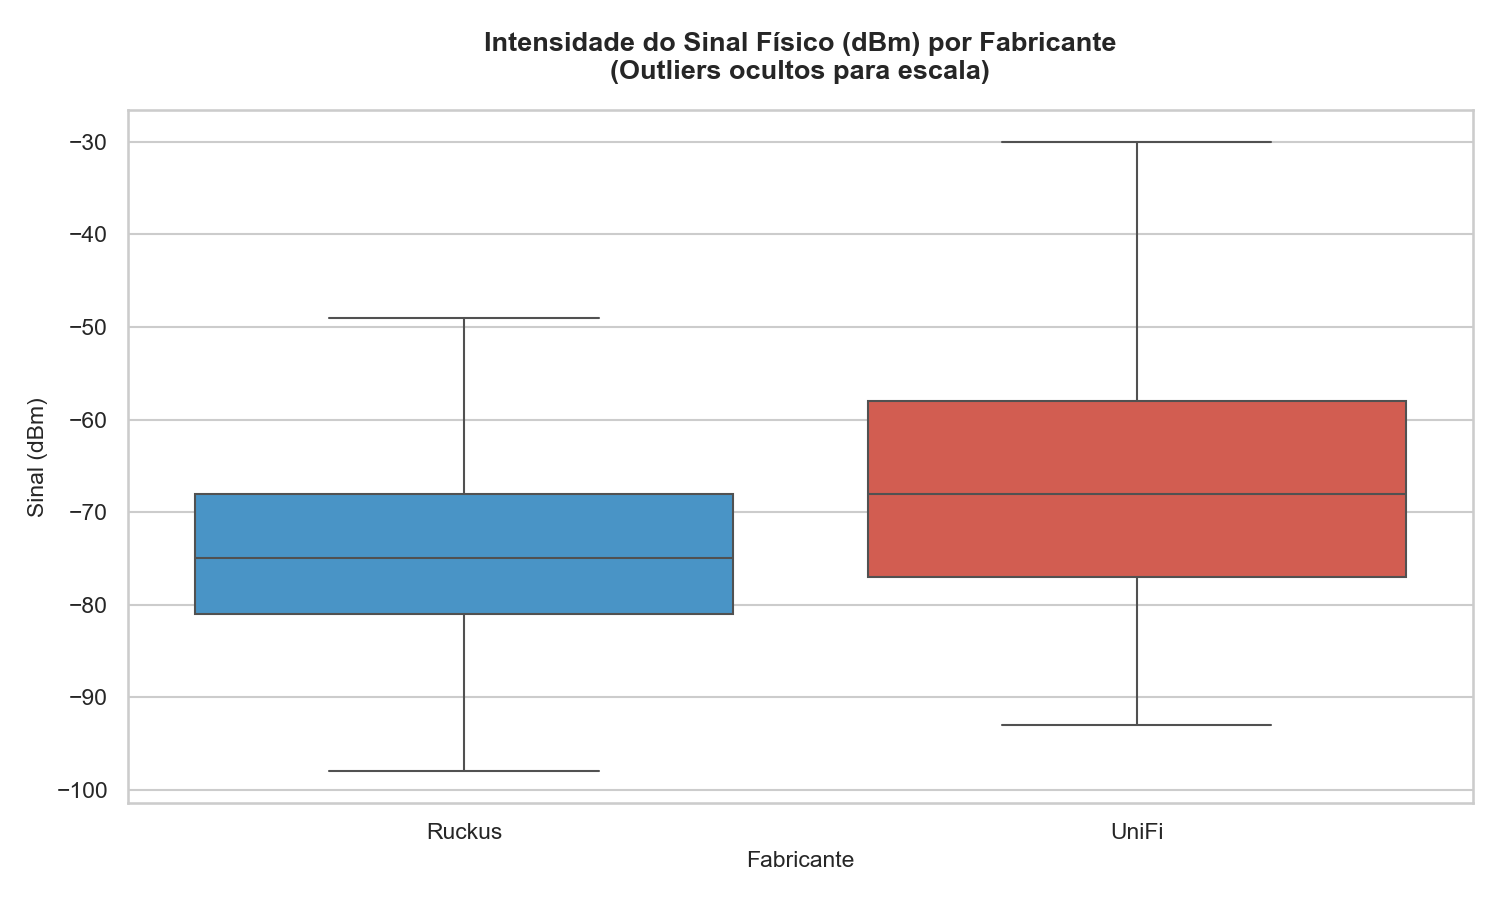
\includegraphics[width=0.85\textwidth]{img/boxplot_rssi_fabricante.png}
  \caption{Boxplot RSSI por Fabricante}
  \label{fig:boxplot_rssi_fabricante_png}
\end{figure}

\begin{itemize}
  \item \textbf{Ruckus}: Média de `-73.83 dBm`, Mediana `-75.00 dBm`.
  \item \textbf{UniFi}: Média de `-67.08 dBm`, Mediana `-68.00 dBm`.
  \item Os resultados sugerem uma cobertura de sinal física coerente para os clientes de ambas as marcas no cenário analisado, com a maioria das amostras se situando em uma faixa saudável de RF.
\end{itemize}

\subsubsection{Histograma de Densidade de Sinal}
O histograma apresenta a densidade de ocorrência de potência de sinal nos logs coletados.

\begin{figure}[H]
  \centering
  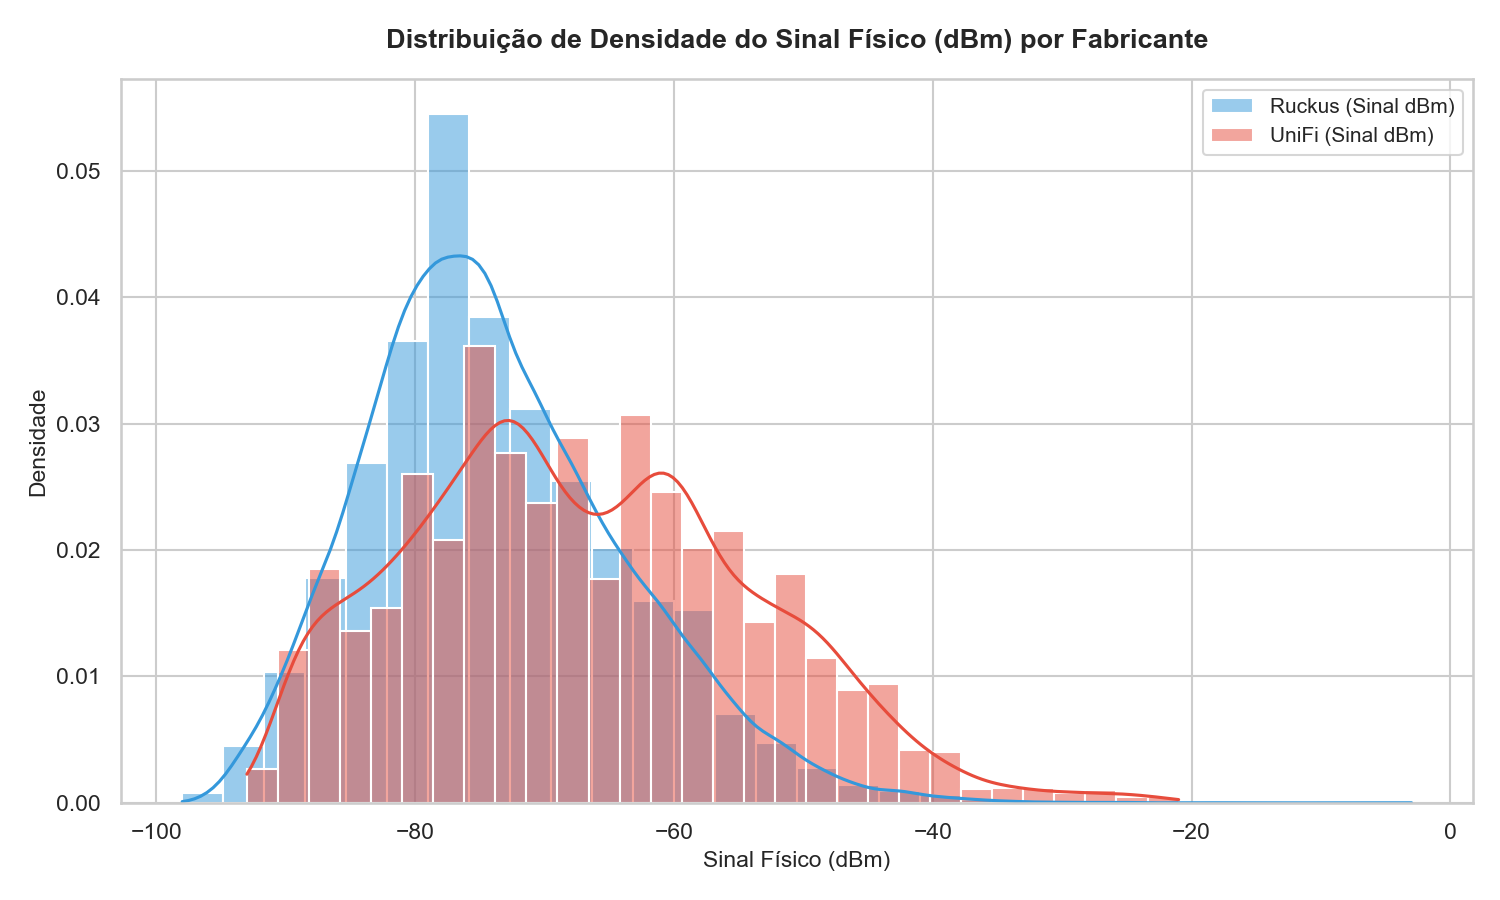
\includegraphics[width=0.85\textwidth]{img/histograma_rssi.png}
  \caption{Histograma RSSI}
  \label{fig:histograma_rssi_png}
\end{figure}

\begin{itemize}
  \item O gráfico demonstra que a UniFi possui uma distribuição de sinal com menor variabilidade (concentrada em torno de -67 dBm), enquanto a Ruckus apresenta maior amplitude e dispersão das conexões ao longo do dia.
\end{itemize}


\subsection{Utilização de Canais por Fabricante}

O histograma de utilização de canais apresenta a contagem de registros em cada frequência de operação.

\begin{figure}[H]
  \centering
  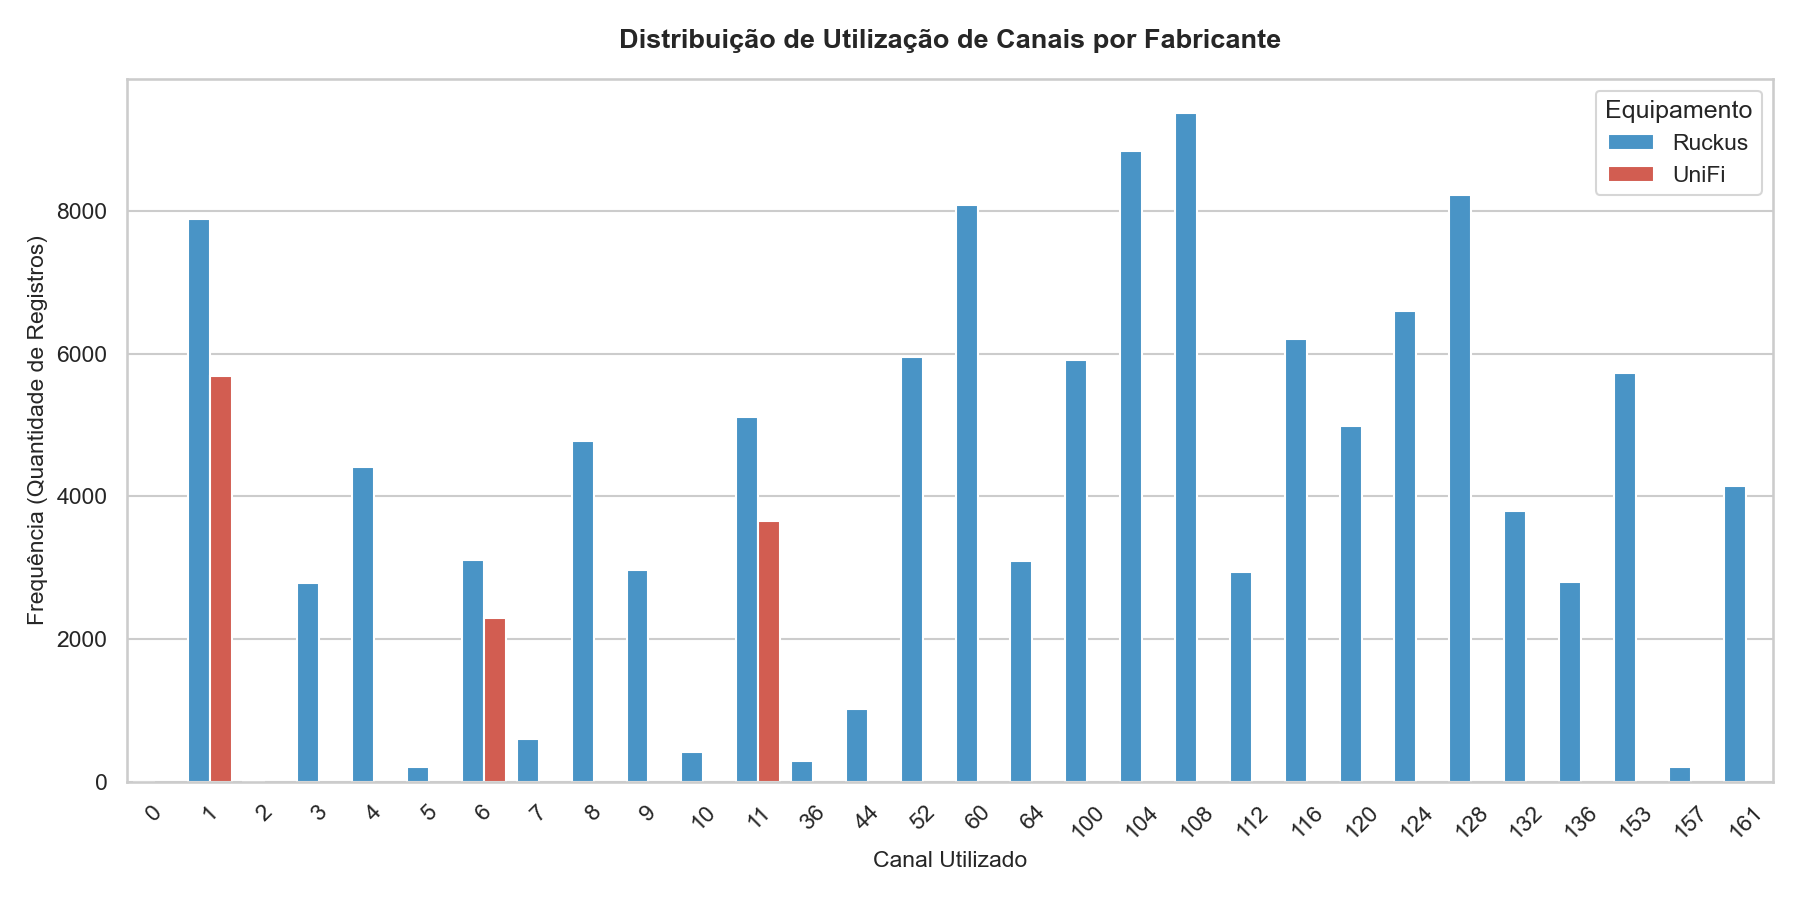
\includegraphics[width=0.85\textwidth]{img/histograma_canais.png}
  \caption{Histograma de Canais}
  \label{fig:histograma_canais_png}
\end{figure}

\begin{itemize}
  \item \textbf{2.4 GHz}: Ambas as marcas concentram o tráfego nos canais não sobrepostos `1`, `6` e `11`, validando as boas práticas de planejamento de RF adotadas no campus.
  \item \textbf{5 GHz}: A Ruckus apresenta uma alocação de espectro mais ampla e distribuída (como canais `36`, `52`, `60`, `104`, `112`, `120`, `128`, `149`), o que reduz interferência co-canal em células adjacentes.
\end{itemize}


\subsection{Quantidade de Clientes Conectados por AP}

Este histograma ilustra a densidade de clientes associados simultaneamente a cada Access Point.

\begin{figure}[H]
  \centering
  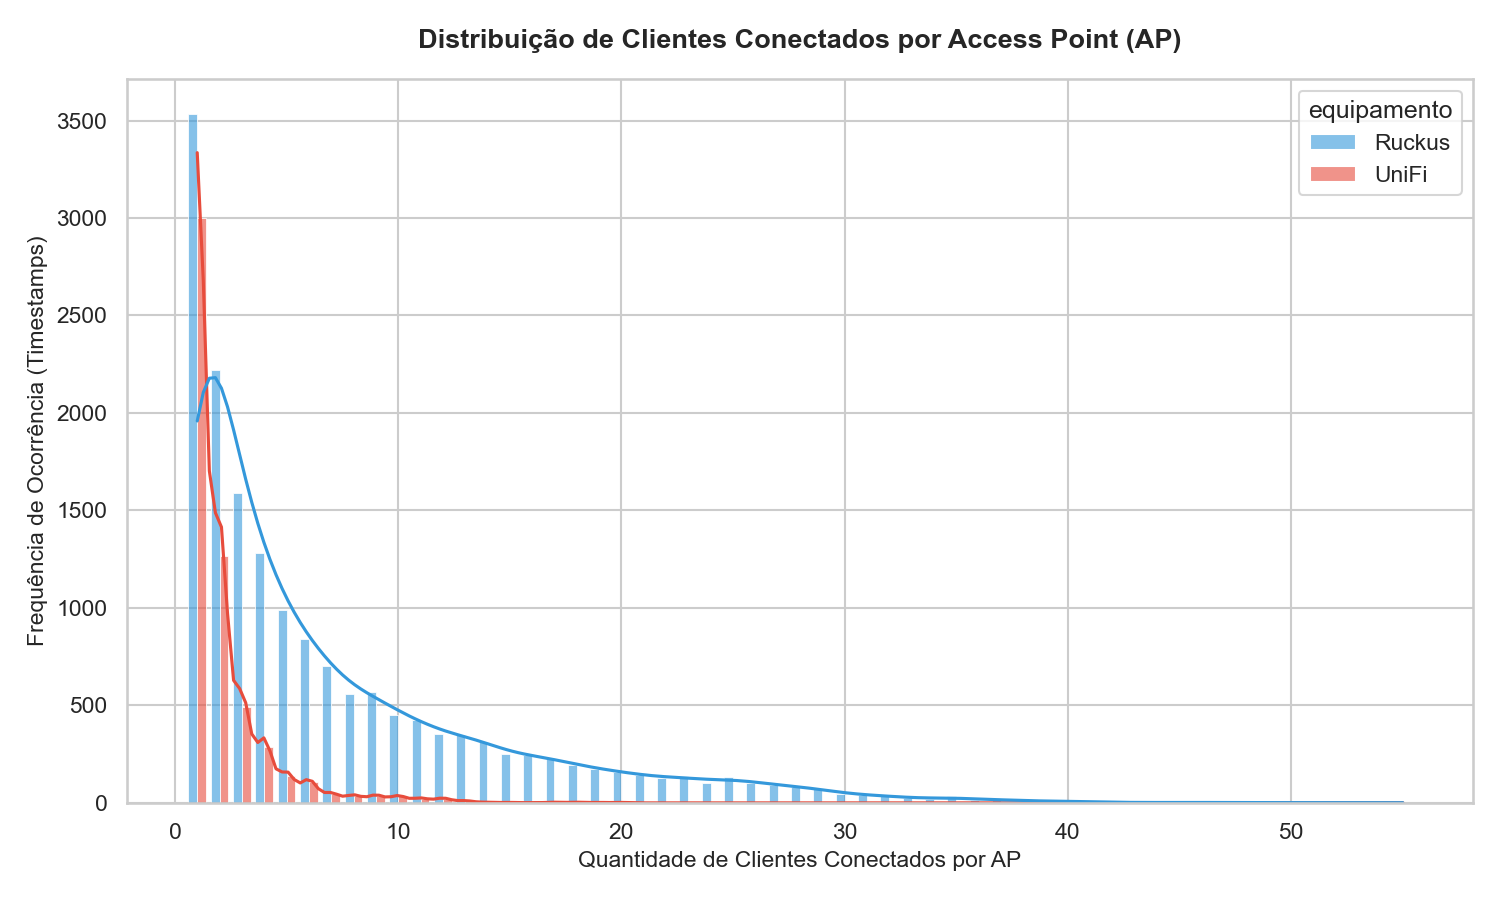
\includegraphics[width=0.85\textwidth]{img/histograma_clientes_por_ap.png}
  \caption{Histograma Clientes por AP}
  \label{fig:histograma_clientes_por_ap_png}
\end{figure}

\begin{itemize}
  \item \textbf{UniFi}: Exibe perfil de baixa carga (maior parte dos registros possui entre 1 e 5 clientes simultâneos por rádio).
  \item \textbf{Ruckus}: Exibe maior flexibilidade de densidade, suportando APs com cargas significativamente mais robustas de concorrência, o que condiz com o posicionamento de alta densidade da marca.
\end{itemize}


\subsection{Análise de Desempenho e Qualidade de Enlace por Banda}

\subsubsection{Throughput por Banda}
O boxplot compara o consumo de throughput entre as bandas de 2.4 GHz e 5 GHz.

\begin{figure}[H]
  \centering
  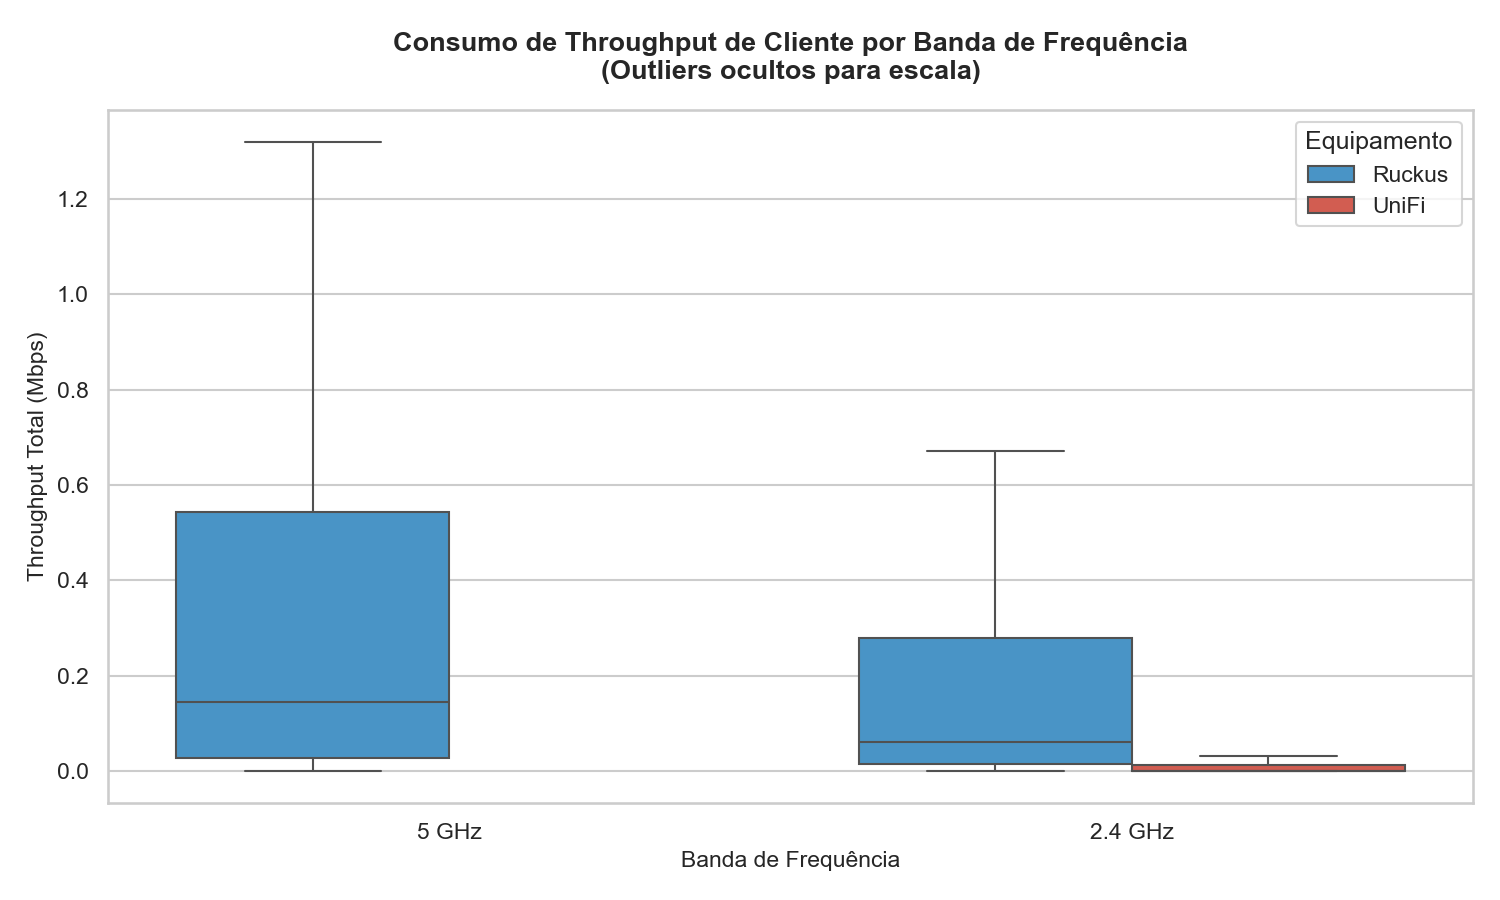
\includegraphics[width=0.85\textwidth]{img/boxplot_throughput_banda.png}
  \caption{Boxplot Throughput por Banda}
  \label{fig:boxplot_throughput_banda_png}
\end{figure}

\begin{itemize}
  \item Como esperado teoricamente, a banda de \textbf{5 GHz} oferece vazão e capacidade física superior para ambas as marcas, superando a banda de \textbf{2.4 GHz} que possui limitações inerentes de modulação e largura de canal.
\end{itemize}

\subsubsection{Retransmissões por Banda}
O boxplot compara a ocorrência de retransmissões físicas ou estimadas.

\begin{figure}[H]
  \centering
  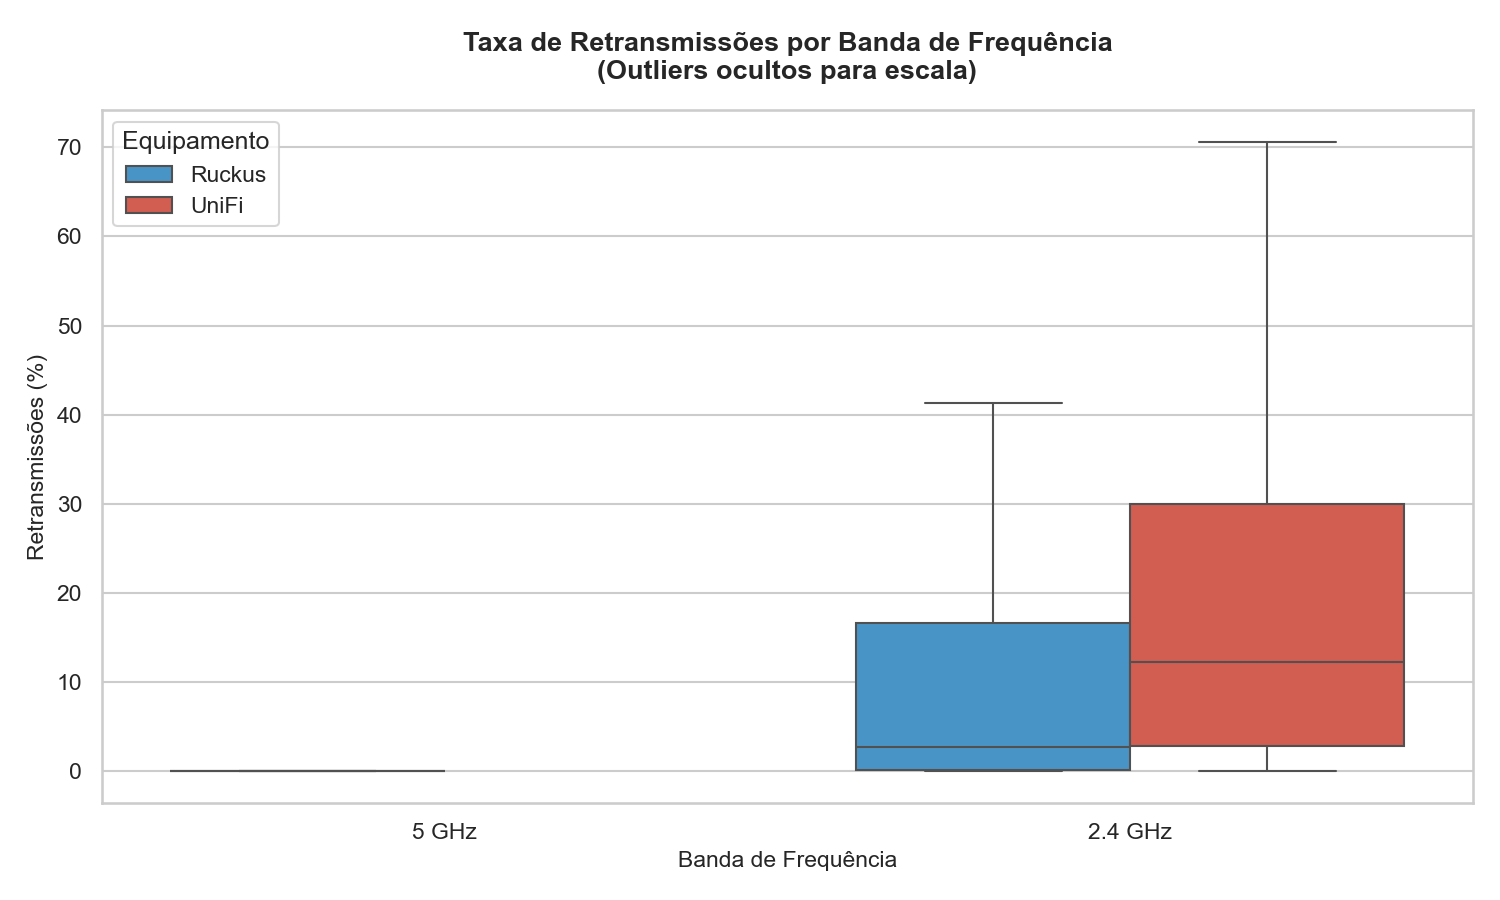
\includegraphics[width=0.85\textwidth]{img/boxplot_retransmissoes_banda.png}
  \caption{Boxplot Retransmissões por Banda}
  \label{fig:boxplot_retransmissoes_banda_png}
\end{figure}

\begin{itemize}
  \item A banda de \textbf{2.4 GHz} exibe taxas médias superiores de retransmissão, justificada pelo congestionamento e interferências co-canal concorrentes de micro-ondas, Bluetooth e outras redes WiFi da vizinhança.
\end{itemize}


\subsection{Distribuição de Throughput Agregado por AP}

Este gráfico apresenta a soma da vazão ativa de todos os clientes associados a cada um dos APs mapeados, permitindo identificar o nível de carregamento individual de tráfego por antena.

\begin{figure}[H]
  \centering
  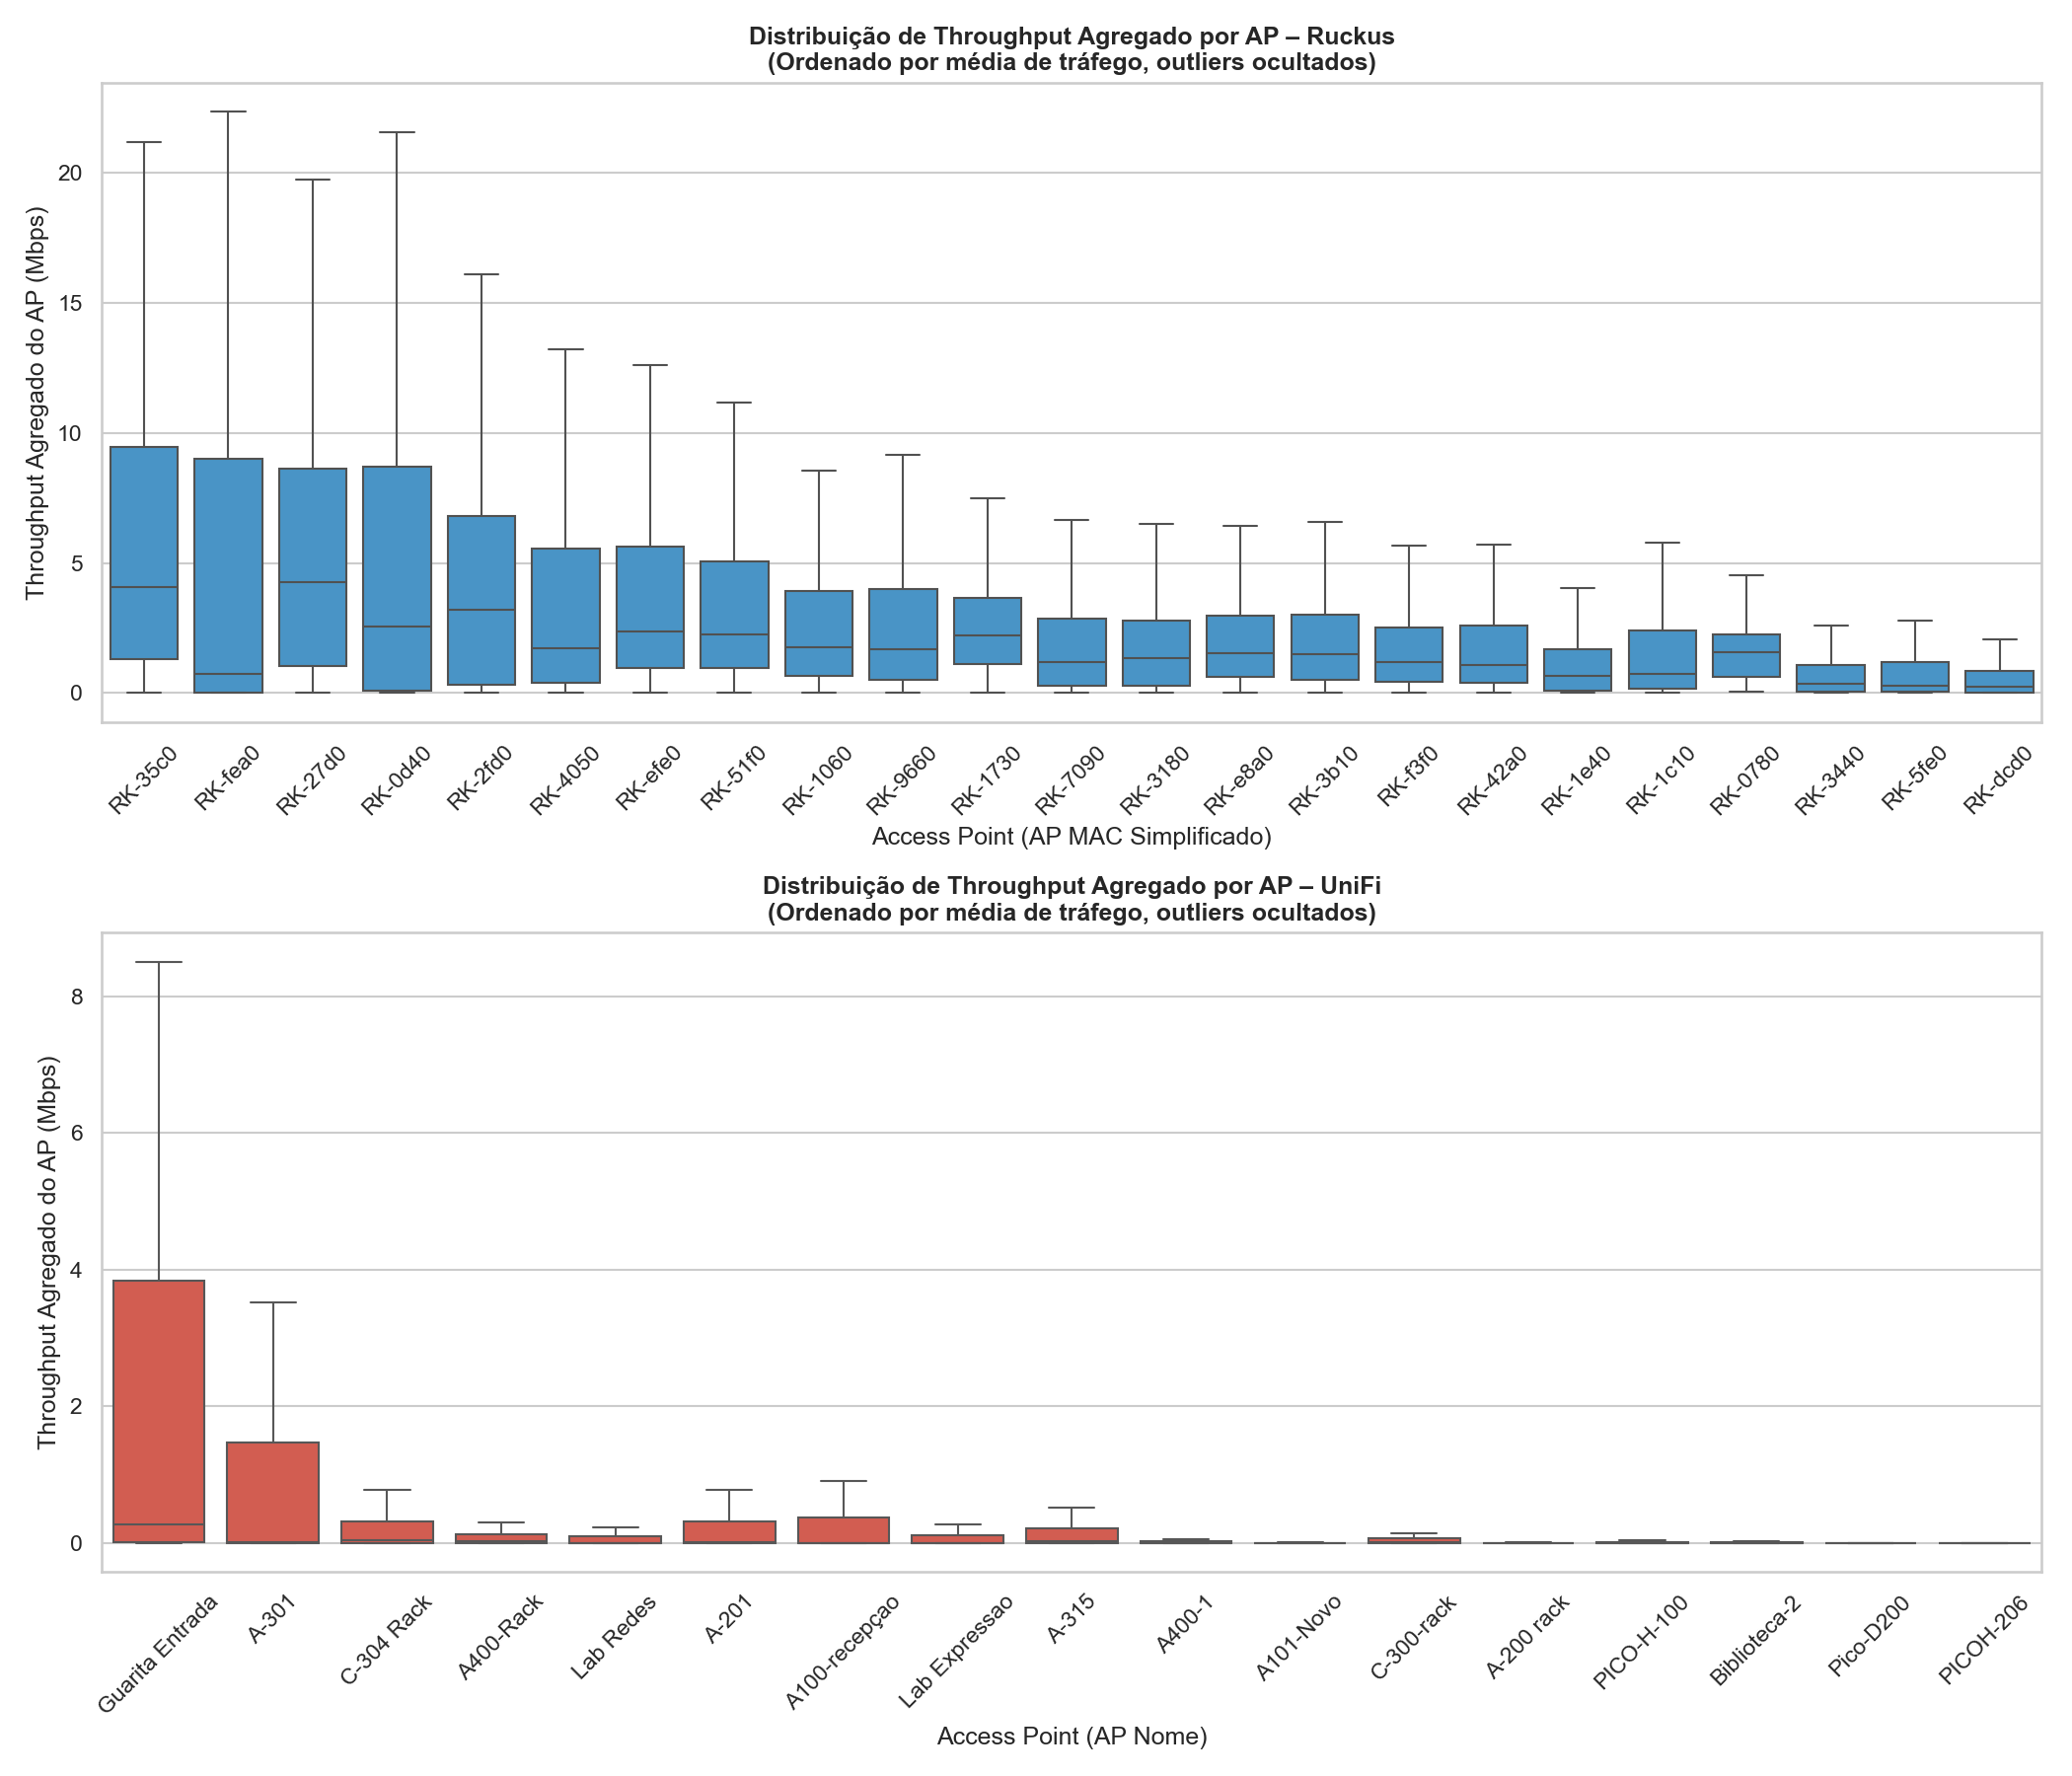
\includegraphics[width=0.85\textwidth]{img/boxplot_throughput_por_ap.png}
  \caption{Boxplot Throughput por AP}
  \label{fig:boxplot_throughput_por_ap_png}
\end{figure}

\begin{itemize}
  \item \textbf{Ruckus (AP MAC Simplificado)}: Apresenta maior amplitude e níveis superiores de vazão somada (vários APs superando médias de 5 a 10 Mbps de tráfego agregado ativo, com picos de consumo expressivos). Para melhor visualização, os endereços MAC longos do Ruckus foram simplificados no formato `RK-XXXX` (onde `XXXX` são os 4 dígitos finais do MAC).
  \item \textbf{UniFi (AP Nome)}: Mostra distribuições de vazão agregada concentradas próximas de zero (com médias inferiores a 2 Mbps). Isso indica que a maioria dos APs da UniFi operaram com carga de dados muito baixa durante o período amostrado, corroborando a ociosidade do ambiente.
\end{itemize}


\subsection{Distribuição Temporal de Clientes Únicos por Fabricante e Dia}

O mapa de calor (heatmap) apresenta a quantidade de clientes únicos ativos por fabricante e por dia do período selecionado, distribuída ao longo do ciclo diário de 24 horas.

\begin{figure}[H]
  \centering
  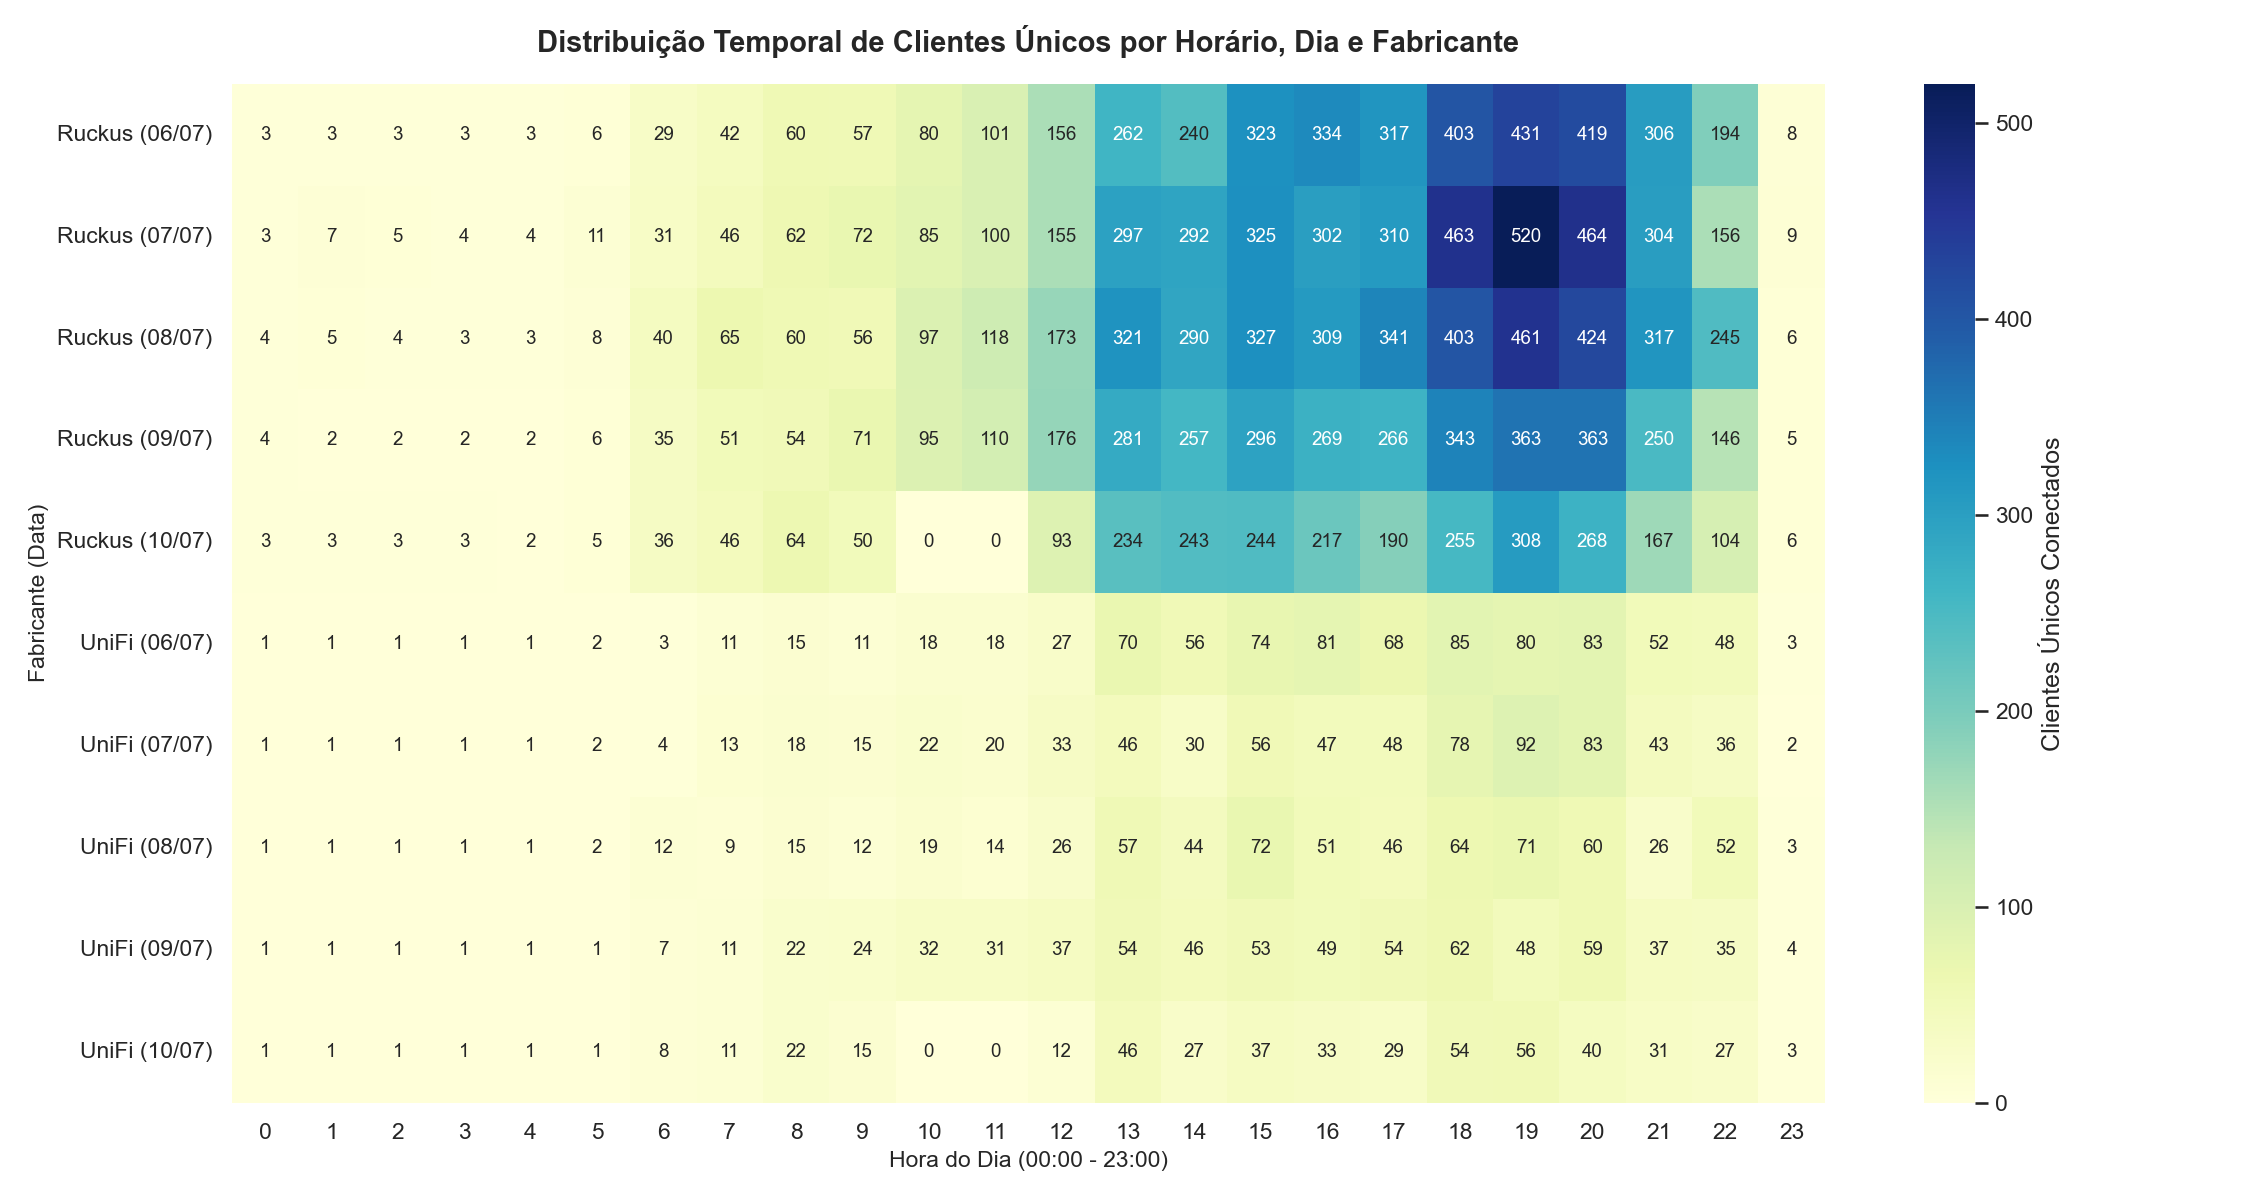
\includegraphics[width=0.85\textwidth]{img/heatmap_horario_clientes.png}
  \caption{Heatmap de Clientes Únicos}
  \label{fig:heatmap_horario_clientes_png}
\end{figure}

\begin{itemize}
  \item O gráfico sugere uma \textbf{rotina cíclica de uso da rede} que se repete de forma semelhante ao longo dos dias: o volume de clientes únicos ativos inicia uma curva ascendente a partir das \textbf{08:00}, atinge os maiores patamares no horário comercial/acadêmico (especialmente entre \textbf{14:00} e \textbf{18:00}) e entra em declínio progressivo nas primeiras horas da noite, reduzindo-se drasticamente durante a madrugada.
  \item \textbf{Picos de Clientes}:
  \item No ambiente Ruckus, o pico de clientes únicos em uma única hora ocorreu no dia \textbf{07/07} às \textbf{19:00}, registrando \textbf{520} dispositivos.
  \item No ambiente UniFi, o pico de clientes únicos ocorreu no dia \textbf{07/07} às \textbf{19:00}, registrando \textbf{92} dispositivos.
  \item Os resultados indicam uma concentração consistentemente maior de dispositivos na infraestrutura Ruckus para todos os dias do período em comparação com a UniFi, o que sugere maior adensamento de usuários sob essa rede no campus observado.
\end{itemize}


\section{Análise de Correlações}

Este relatório apresenta e analisa os coeficientes de correlação de \textbf{Pearson (\textit{r\_p})} e \textbf{Spearman (\textit{r\_s})} e gera gráficos correspondentes para analisar quantitativamente o comportamento da telemetria das redes UniFi e Ruckus.

\textbf{Limitação do Escopo}: As discussões e conclusões apresentadas neste relatório baseiam-se estritamente no cenário e conjunto de dados observados durante o período de coleta. Os resultados sugerem tendências e comportamentos de rede nesse ambiente específico, não devendo ser interpretados como regras gerais absolutas.

Os coeficientes de Pearson medem a força de uma relação linear, enquanto os de Spearman medem a relação monotônica (útil para distribuições não-normais e não-lineares). Ambos variam de -1 a +1. Os símbolos `\textit{` representam significância estatística de }p\textit{ < 0.05 e `\textsuperscript{**}` representam }p\textsuperscript{*} < 0.01.

\subsection{Tabela Consolidada de Coeficientes de Pearson (\textit{r\_p}) e Spearman (\textit{r\_s})}

\begin{table}[htb]
\IBGEtab{%
  \caption{Dados comparativos da análise - Análise de Correlações (Tabela 1)}%
  \label{tab:data_analise_de_correlacoes_1}%
}{%
  \resizebox{\textwidth}{!}{%
    \begin{tabular}{lcccccc}
      \toprule
      Relação Investigada & Ruckus (\textit{r\_p}) & Ruckus (\textit{r\_s}) & Amostras (\textit{N}) & UniFi (\textit{r\_p}) & UniFi (\textit{r\_s}) & Amostras (\textit{N}) \\
      \midrule
      \textbf{RSSI x Throughput Total} & -0.0086\textsuperscript{**} & 0.0363\textsuperscript{**} & 107726 & 0.2305\textsuperscript{**} & 0.4512\textsuperscript{**} & 11641 \\
      \textbf{RSSI x Retransmissoes} & 0.0215\textsuperscript{**} & 0.1642\textsuperscript{**} & 107726 & -0.3437\textsuperscript{**} & -0.3660\textsuperscript{**} & 11641 \\
      \textbf{Retransmissoes x Throughput Total} & -0.1009\textsuperscript{**} & -0.0768\textsuperscript{**} & 120510 & -0.0989\textsuperscript{**} & -0.1321\textsuperscript{**} & 11641 \\
      \textbf{Qtd Clientes x Throughput Agregado AP} & 0.6953\textsuperscript{**} & 0.7962\textsuperscript{**} & 16708 & 0.3310\textsuperscript{**} & 0.5253\textsuperscript{**} & 5506 \\
      \textbf{Qtd Clientes x Retransmissoes Medias AP} & -0.0590\textsuperscript{**} & 0.3572\textsuperscript{**} & 16708 & 0.1081\textsuperscript{**} & 0.2302\textsuperscript{**} & 5506 \\
      \textbf{Noise x Retransmissoes} & -0.3952\textsuperscript{**} & -0.6323\textsuperscript{**} & 107726 & 0.0447\textsuperscript{**} & -0.0043 & 11641 \\
      \textbf{Noise x RSSI} & -0.3933\textsuperscript{**} & -0.3762\textsuperscript{**} & 107726 & 0.1053\textsuperscript{**} & 0.0083 & 11641 \\
      \textbf{Link Speed TX x Throughput TX} & 0.1086\textsuperscript{**} & 0.5475\textsuperscript{**} & 112719 & 0.0536\textsuperscript{**} & 0.2877\textsuperscript{**} & 11641 \\
      \textbf{Volume Total x Tempo de Sessao} & 0.3417\textsuperscript{**} & 0.6861\textsuperscript{**} & 120510 & 0.0980\textsuperscript{**} & 0.3121\textsuperscript{**} & 11641 \\
      \bottomrule
    \end{tabular}%
  }%
}{%
  \fonte{Produzido pelos autores.}%
}
\end{table}


\subsection{Matrizes de Correlação (Heatmap Geral)}

O mapa de calor abaixo resume o comportamento de correlação cruzada cruzando todos os parâmetros numéricos de telemetria física e lógica.

\begin{figure}[H]
  \centering
  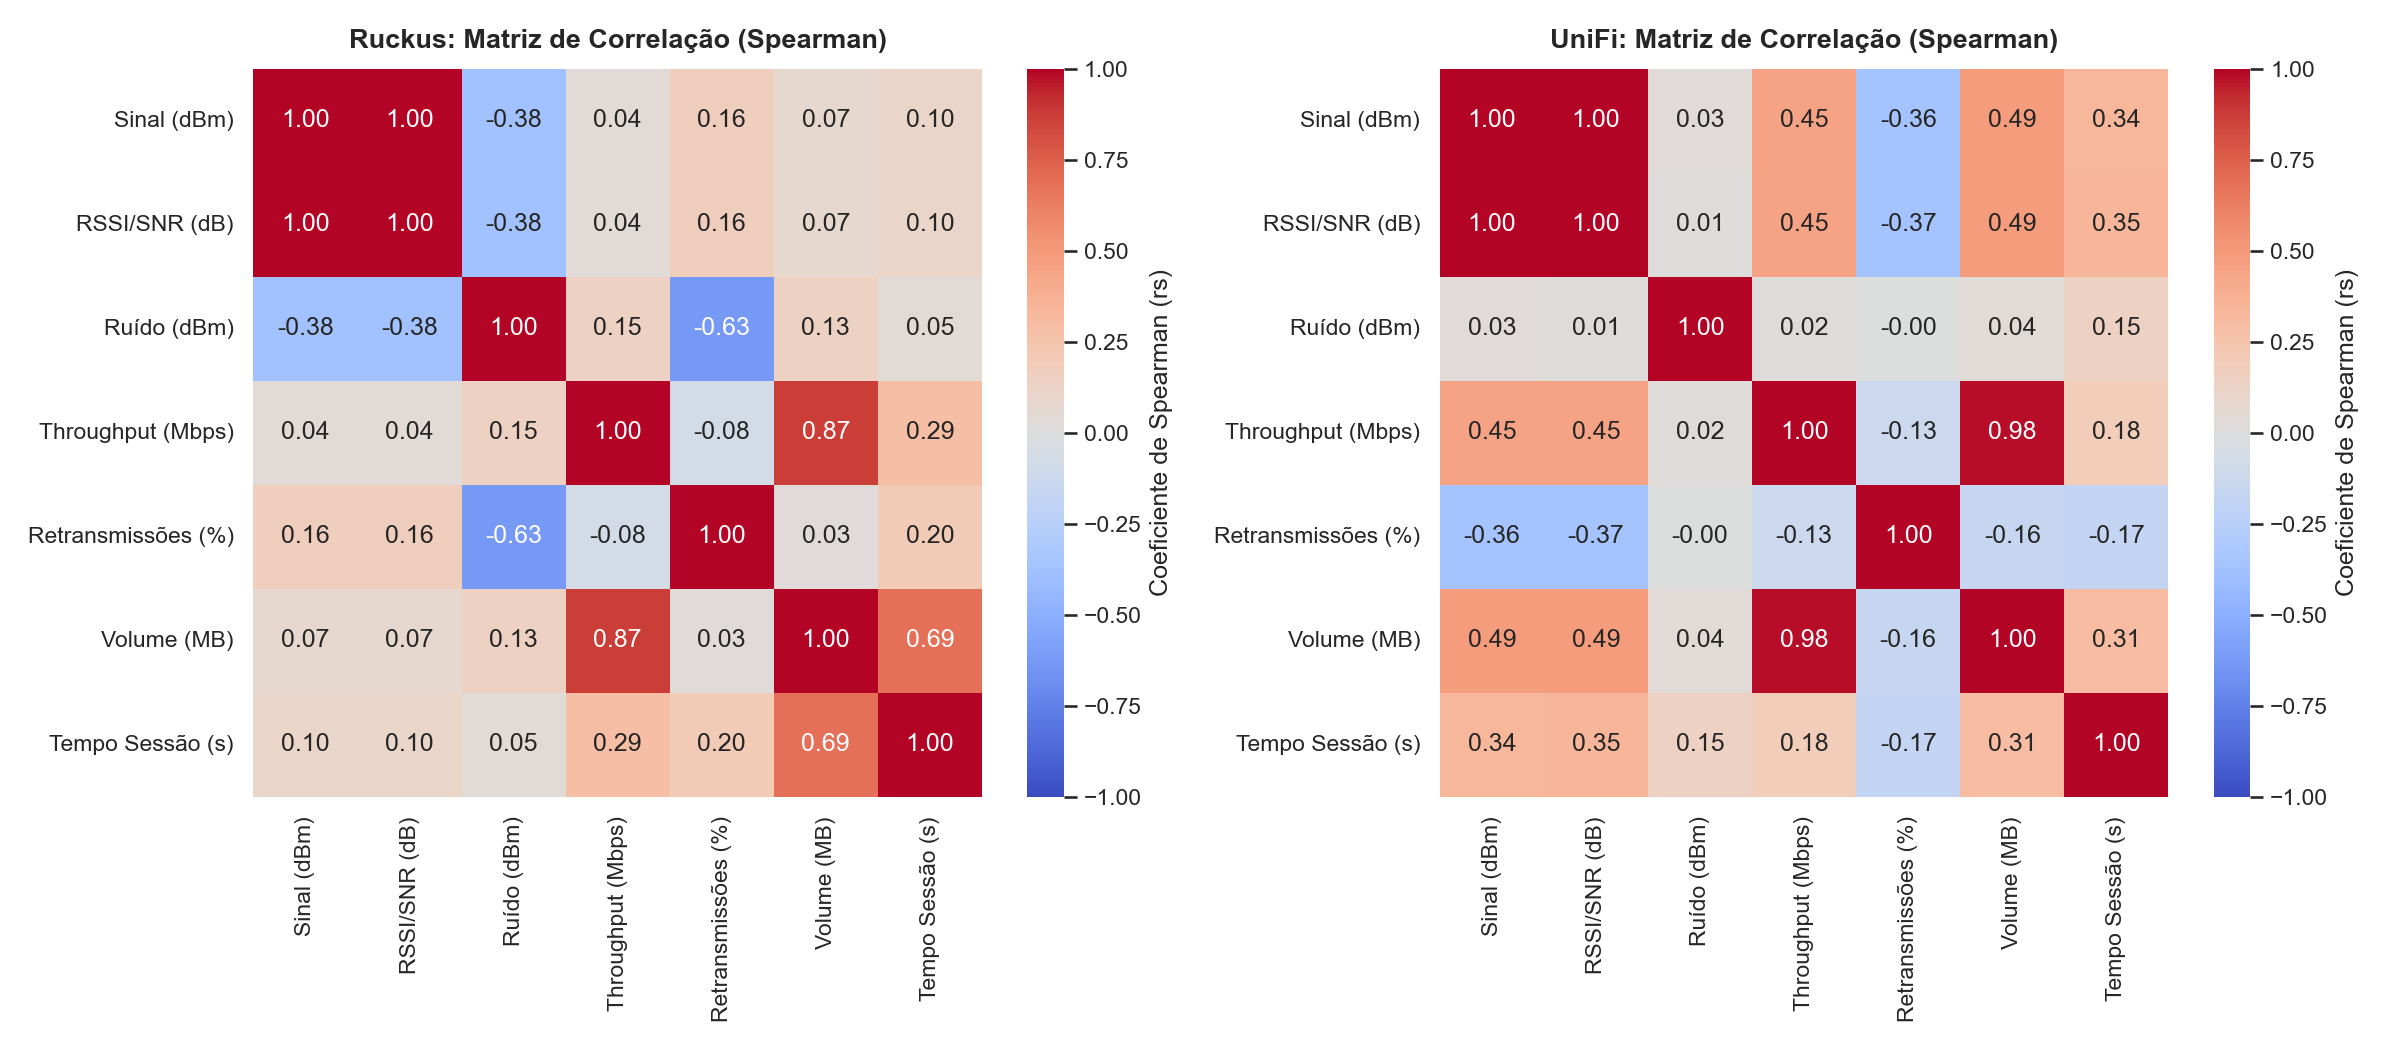
\includegraphics[width=0.85\textwidth]{img/matriz_correlacao_heatmap.png}
  \caption{Matriz de Correlação Heatmap}
  \label{fig:matriz_correlacao_heatmap_png}
\end{figure}

\begin{itemize}
  \item \textbf{Ruckus}: Exibe correlações monotônicas muito fortes entre Sinal e RSSI (sendo a mesma grandeza física mapeada) e o forte acoplamento linear artificial entre Ruído (Noise) e Sinal derivado do método de cálculo. O Throughput dos clientes individuais apresenta baixíssima correlação com a potência do sinal (\textit{r\_s} = 0.0363), condizente com o comportamento de ociosidade predominante.
  \item \textbf{UniFi}: O sinal absoluto (signal) e o RSSI (que atua como índice SNR) exibem correlação positiva moderada a forte (\textit{r\_s} = 0.70). O Throughput individual também apresenta correlação extremamente baixa com a intensidade de sinal (\textit{r\_s} = 0.4512). O ruído de fundo (noise) exibe baixíssima correlação com o sinal, validando a física do meio.
\end{itemize}


\subsection{Análise de Cada Gráfico de Dispersão}

\subsubsection{RSSI × Throughput}
\begin{itemize}
  \item \textbf{Arquivo}: `01\_rssi\_throughput.png`
  \item \textbf{Visualização}:
\end{itemize}
\begin{figure}[H]
  \centering
  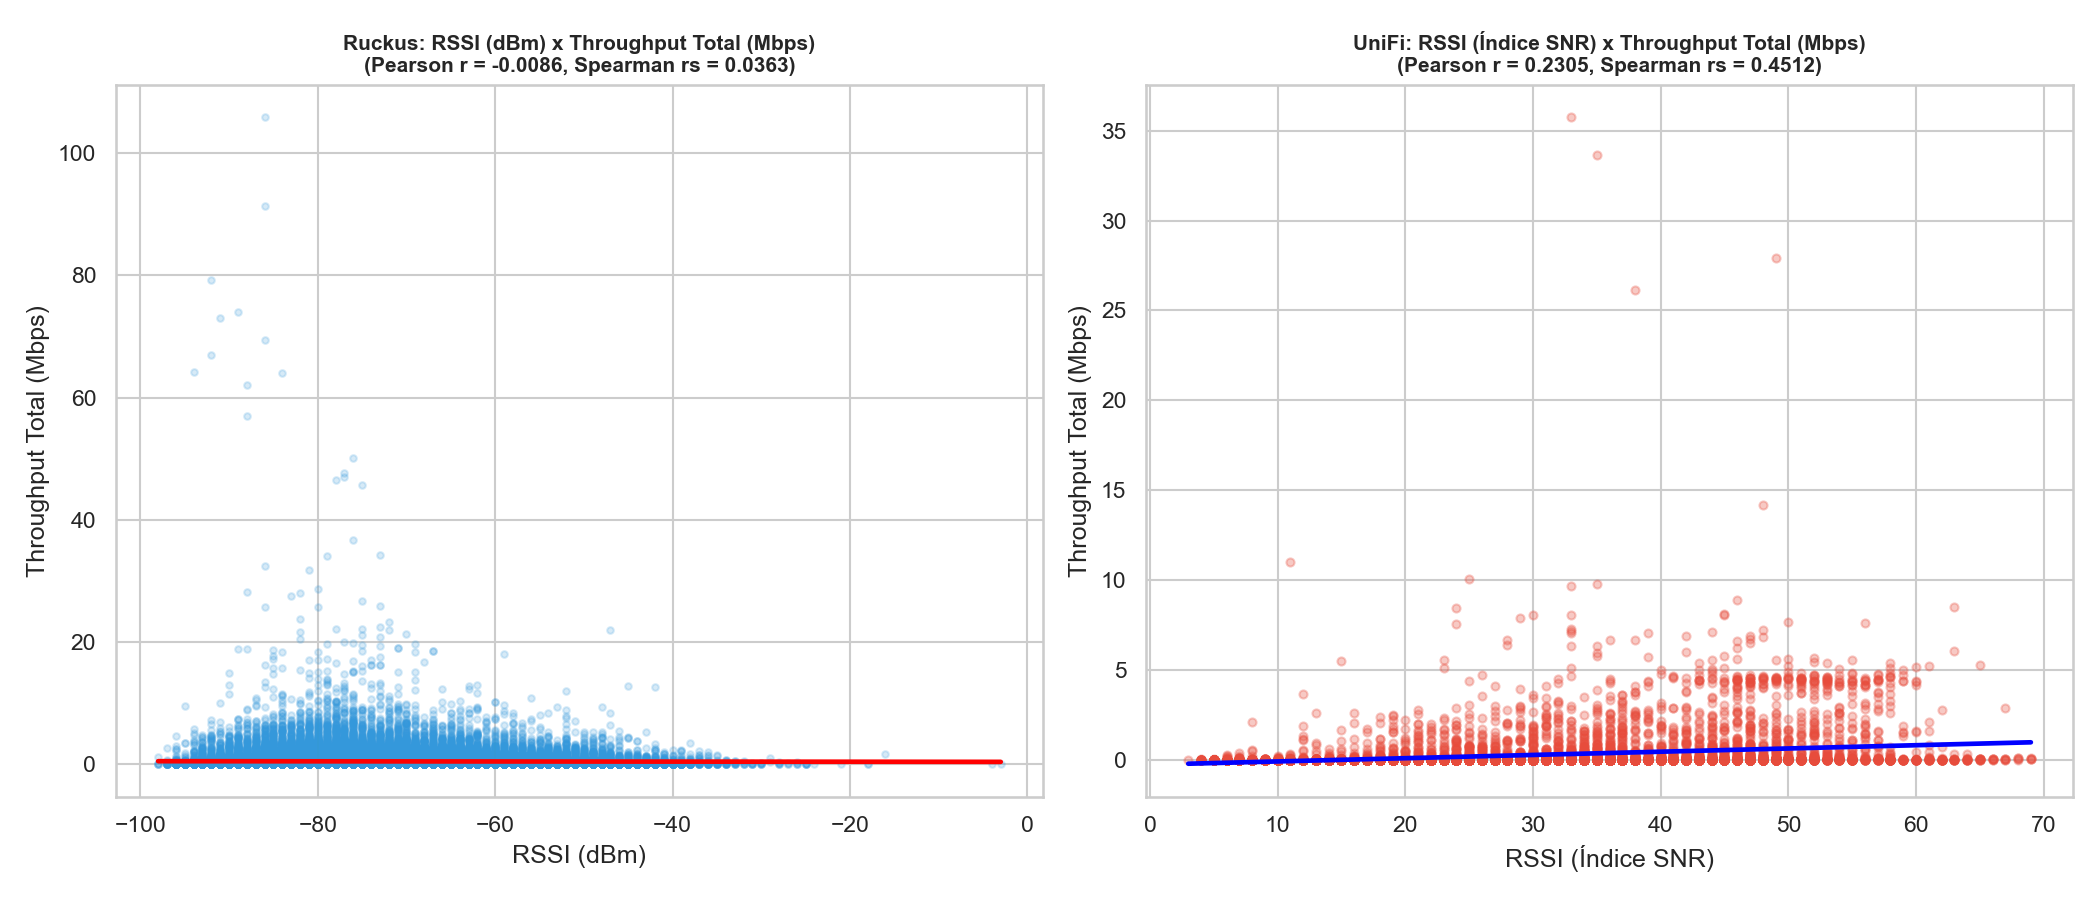
\includegraphics[width=0.85\textwidth]{img/01_rssi_throughput.png}
  \caption{RSSI x Throughput}
  \label{fig:01_rssi_throughput_png}
\end{figure}
\begin{itemize}
  \item \textbf{Expectativa Teórica}: Esperava-se uma correlação positiva moderada a forte. Sinais com melhor intensidade (RSSI alto) permitem modulações e taxas físicas maiores, o que deveria se traduzir em taxas mais altas de transferência ativa.
  \item \textbf{Comportamento Observado}: Os dados sugerem correlação praticamente nula no Ruckus (\textit{r\_p} = -0.0086, \textit{r\_s} = 0.0363) e fraca na UniFi (\textit{r\_p} = 0.2305, \textit{r\_s} = 0.4512).
  \item \textbf{Discussão}: Esta divergência sugere que o throughput de dados ativo depende fundamentalmente do padrão de demanda do usuário no instante de coleta. A maioria esmagadora dos dispositivos conectados permaneceu ociosa ou gerando tráfego insignificante (background sync), independentemente de estarem com sinal excelente ou intermediário.
\end{itemize}

\subsubsection{RSSI × Retransmissões}
\begin{itemize}
  \item \textbf{Arquivo}: `02\_rssi\_retransmissoes.png`
  \item \textbf{Visualização}:
\end{itemize}
\begin{figure}[H]
  \centering
  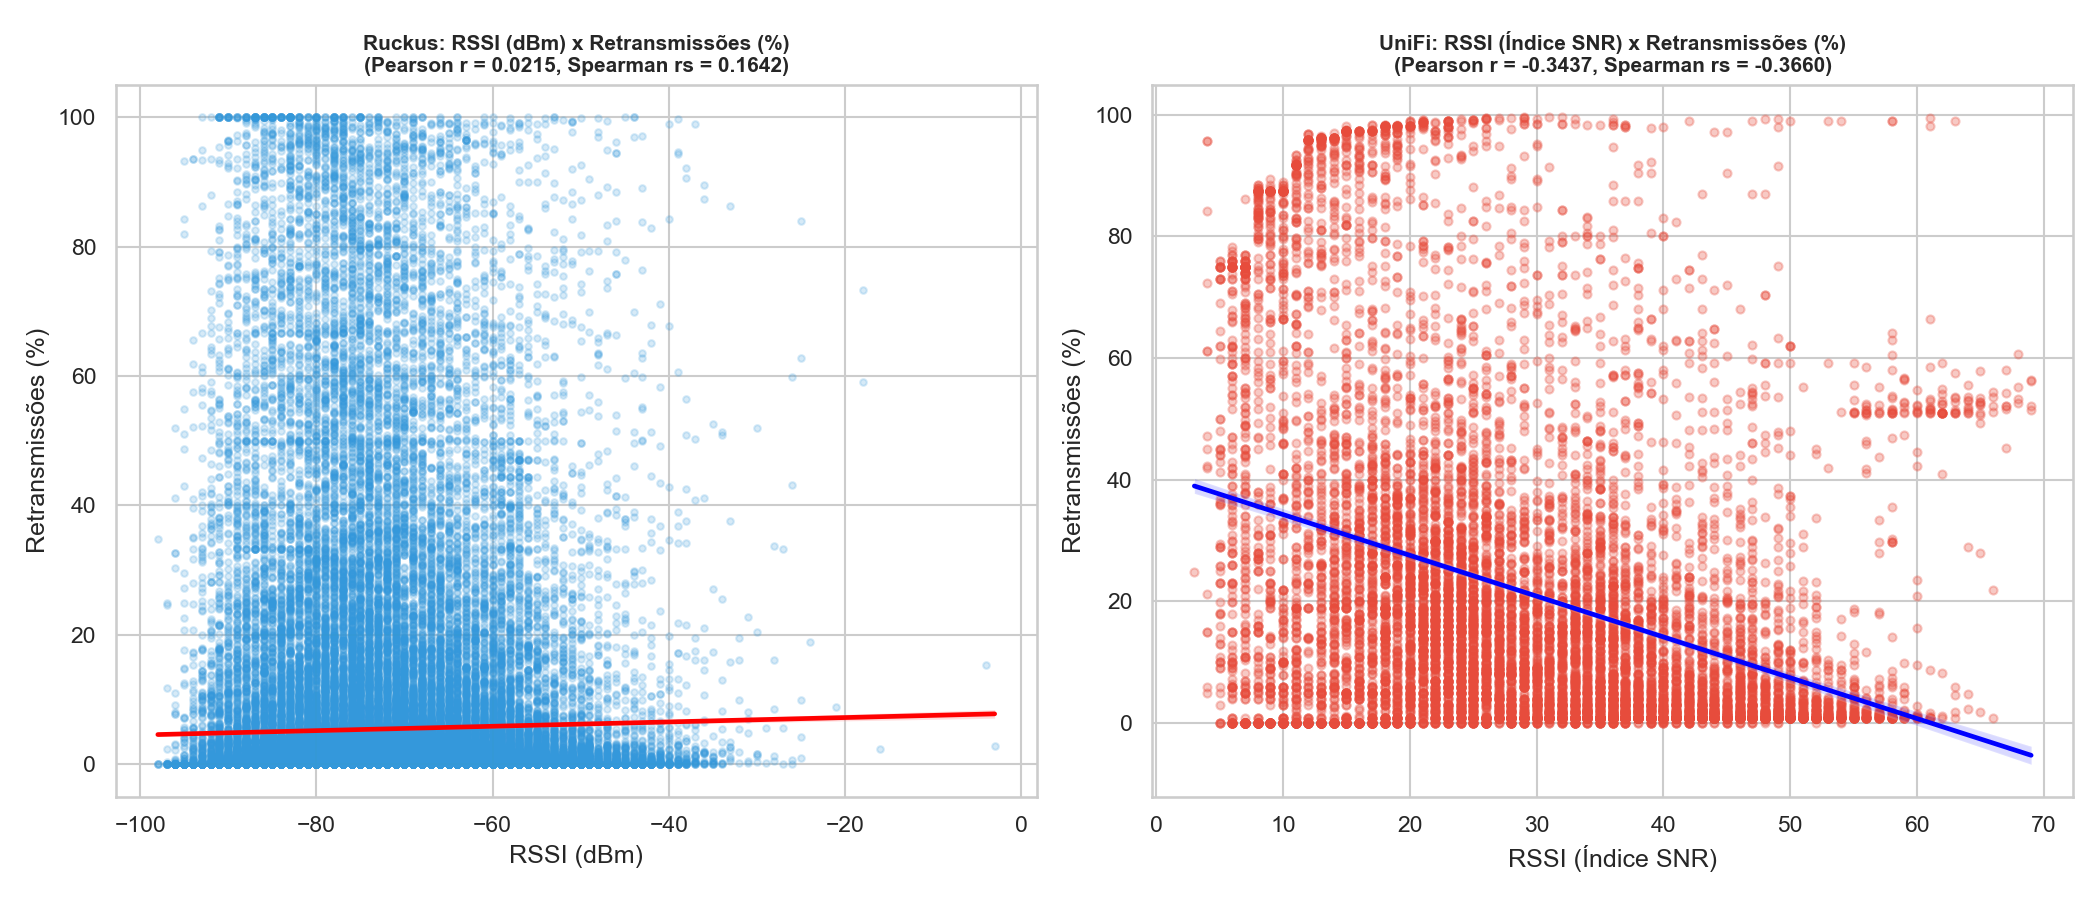
\includegraphics[width=0.85\textwidth]{img/02_rssi_retransmissoes.png}
  \caption{RSSI x Retransmissões}
  \label{fig:02_rssi_retransmissoes_png}
\end{figure}
\begin{itemize}
  \item \textbf{Expectativa Teórica}: Esperava-se uma correlação negativa moderada a forte. Níveis fracos de sinal costumam reduzir o SNR, elevando a taxa de bits incorretos (BER) e gerando retransmissões para recuperar os pacotes.
  \item \textbf{Comportamento Observado}: Correlação negativa muito fraca no Ruckus (\textit{r\_p} = 0.0215, \textit{r\_s} = 0.1642) e negativa moderada na UniFi (\textit{r\_p} = -0.3437, \textit{r\_s} = -0.3660).
  \item \textbf{Discussão}: Os dados da UniFi são consistentes com a teoria de que o sinal fraco prejudica o canal. Na Ruckus, a fraca correlação observada indica a atuação de mecanismos de hardware e software (como antenas inteligentes BeamFlex e controle de potência dinâmico) que evitam a perda excessiva de quadros físicos mesmo em níveis moderadamente baixos de sinal.
\end{itemize}

\subsubsection{Retransmissões × Throughput}
\begin{itemize}
  \item \textbf{Arquivo}: `03\_retransmissoes\_throughput.png`
  \item \textbf{Visualização}:
\end{itemize}
\begin{figure}[H]
  \centering
  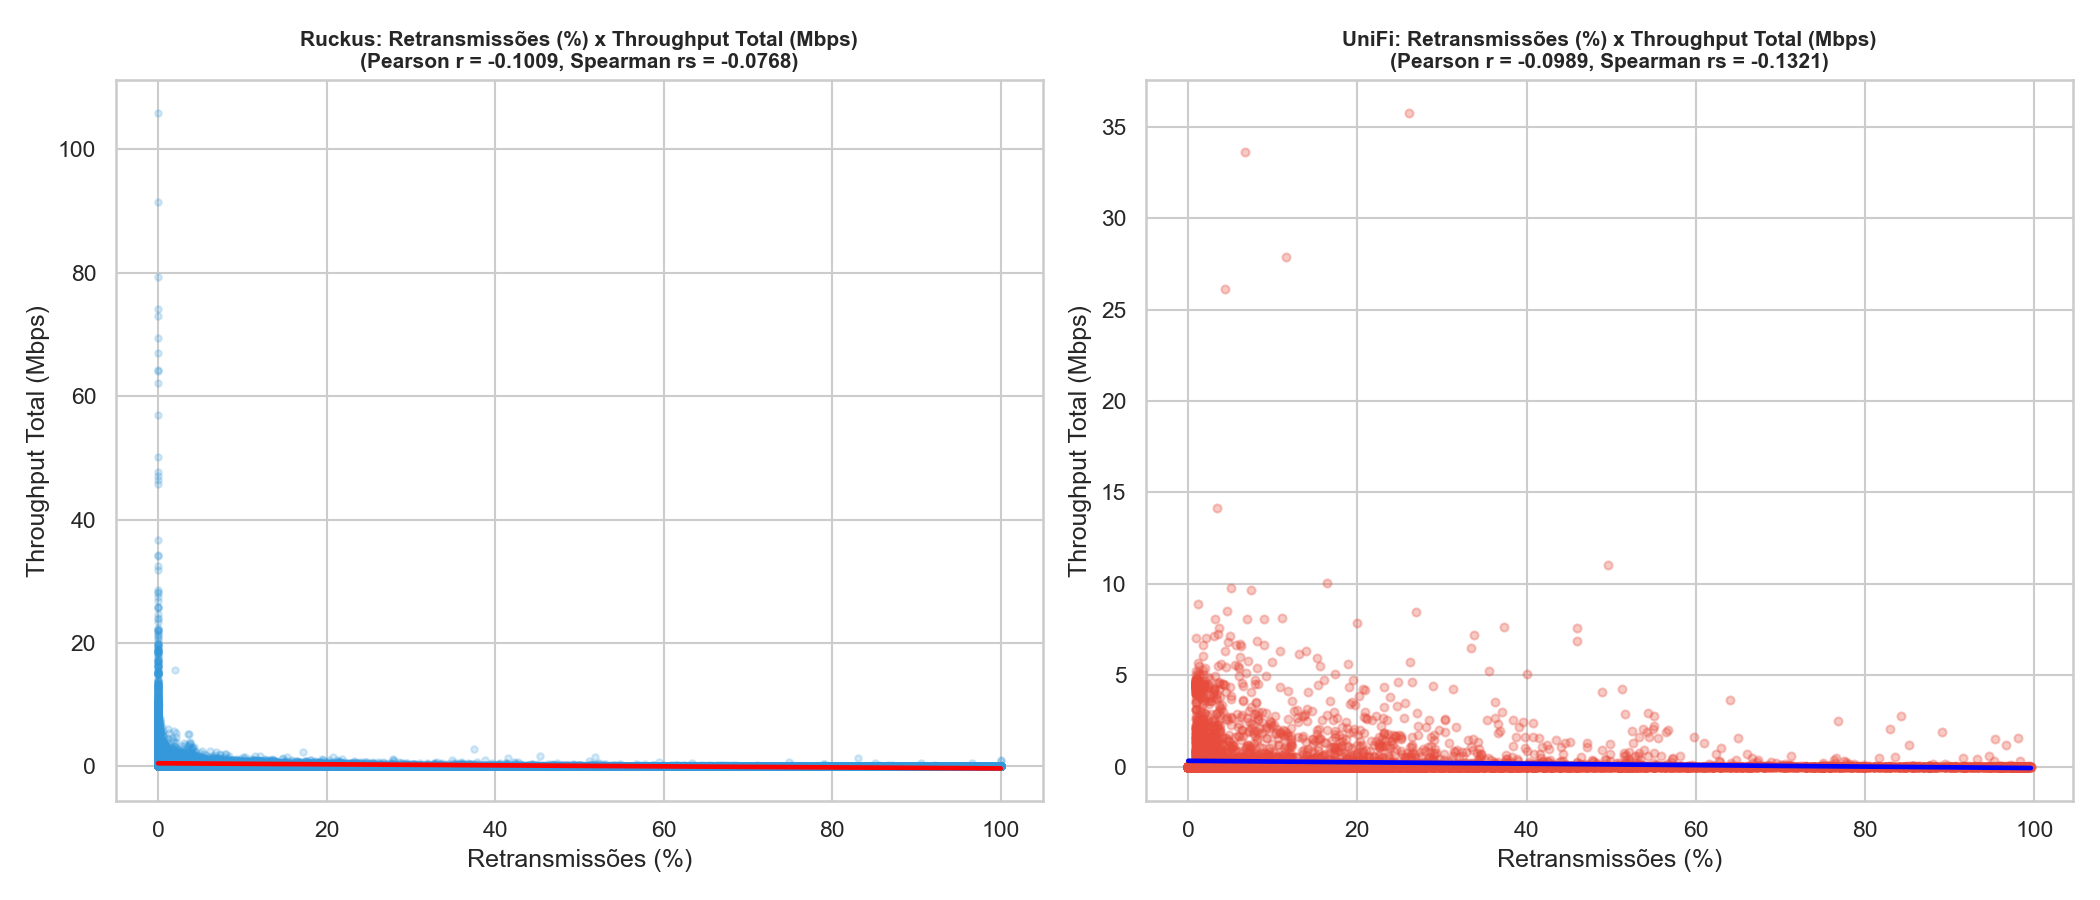
\includegraphics[width=0.85\textwidth]{img/03_retransmissoes_throughput.png}
  \caption{Retransmissões x Throughput}
  \label{fig:03_retransmissoes_throughput_png}
\end{figure}
\begin{itemize}
  \item \textbf{Expectativa Teórica}: Esperava-se uma correlação negativa moderada, pois altas retransmissões consomem tempo de canal de RF (airtime) e reduzem a capacidade útil.
  \item \textbf{Comportamento Observado}: Correlação negativa fraca no Ruckus (\textit{r\_p} = -0.1009, \textit{r\_s} = -0.0768) e na UniFi (\textit{r\_p} = -0.0989, \textit{r\_s} = -0.1321).
  \item \textbf{Discussão}: Os resultados sugerem que, como o throughput ativo na rede está muito longe do teto operacional dos canais (baixa carga ativa), o impacto de retransmissões dispersas no throughput do usuário não se mostrou severo o suficiente para gerar decréscimo drástico na taxa média registrada.
\end{itemize}

\subsubsection{Quantidade de Clientes × Throughput Agregado do AP}
\begin{itemize}
  \item \textbf{Arquivo}: `04\_clientes\_throughput\_ap.png`
  \item \textbf{Visualização}:
\end{itemize}
\begin{figure}[H]
  \centering
  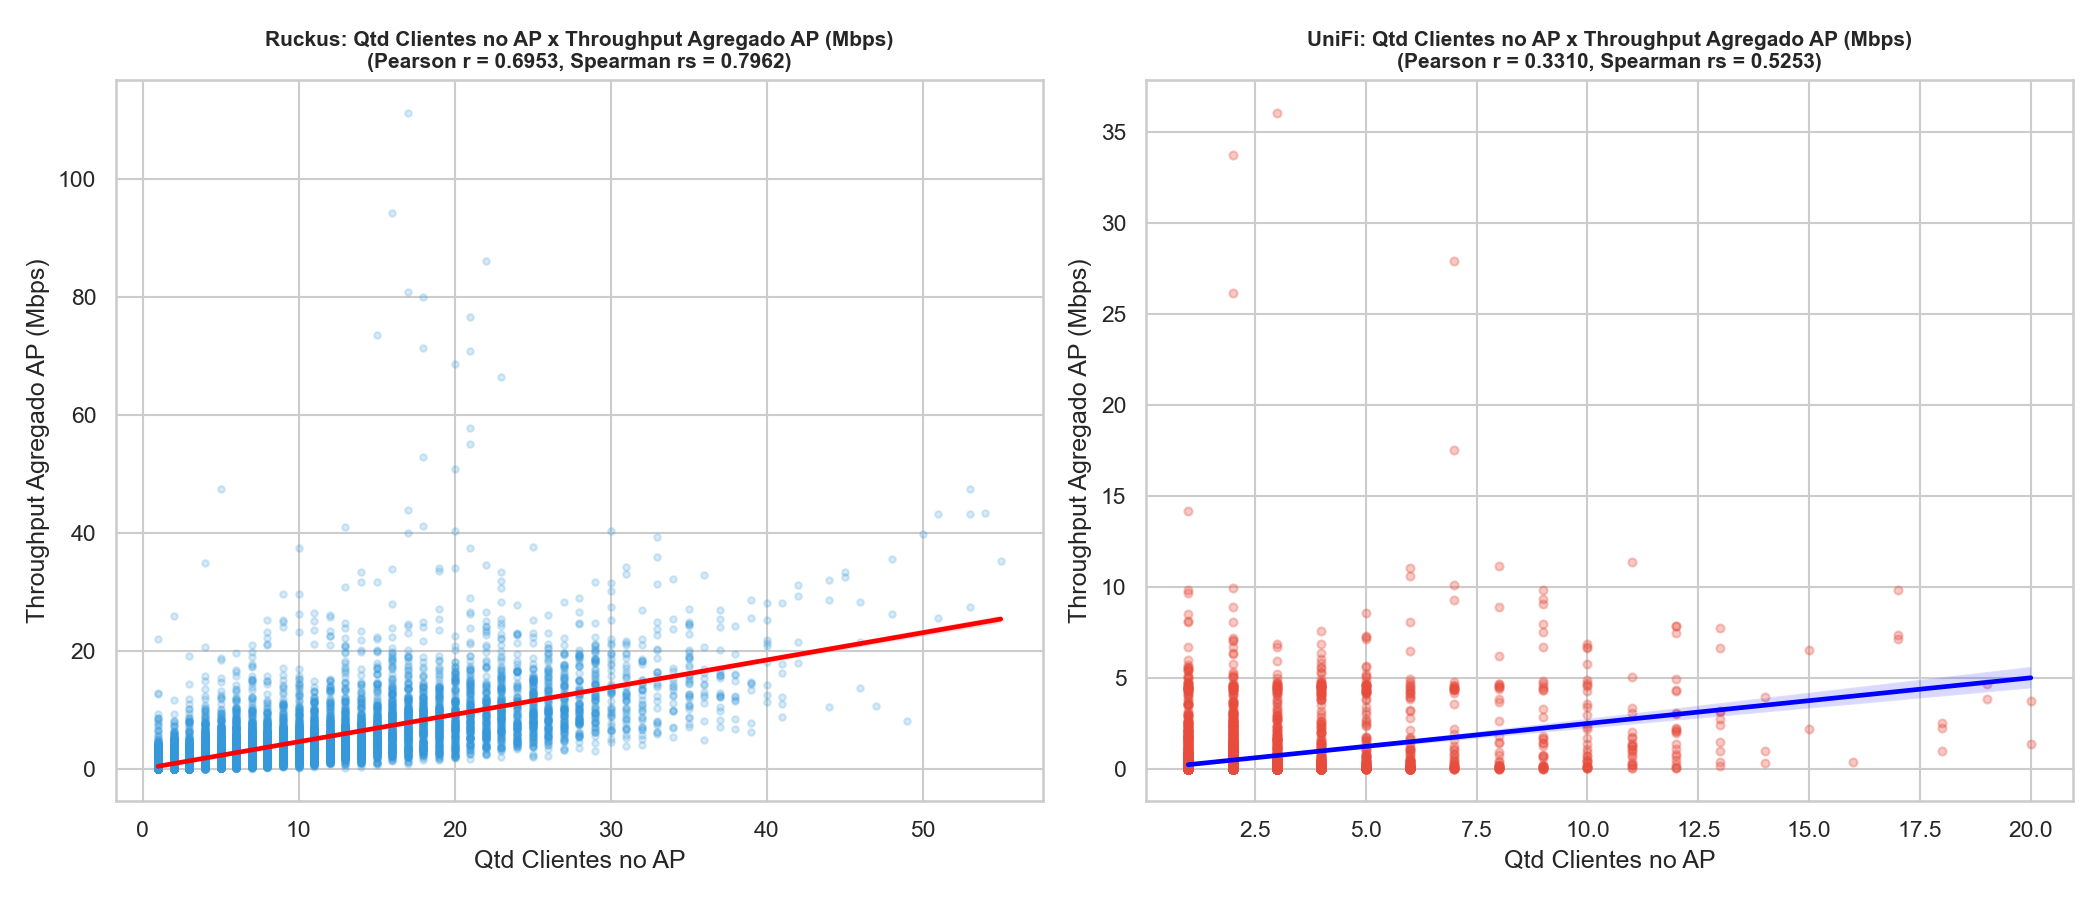
\includegraphics[width=0.85\textwidth]{img/04_clientes_throughput_ap.png}
  \caption{Clientes x Throughput Agregado}
  \label{fig:04_clientes_throughput_ap_png}
\end{figure}
\begin{itemize}
  \item \textbf{Expectativa Teórica}: Esperava-se uma correlação positiva moderada a forte, visto que o tráfego total somado em um AP tende a crescer proporcionalmente com a quantidade de dispositivos ativos gerando tráfego concorrente.
  \item \textbf{Comportamento Observado}: Os dados indicam correlação positiva forte no Ruckus (\textit{r\_p} = 0.6953, \textit{r\_s} = 0.7962) e positiva moderada a forte na UniFi (\textit{r\_p} = 0.3310, \textit{r\_s} = 0.5253).
  \item \textbf{Discussão}: Esse resultado é consistente com o esperado teoricamente. O tráfego consolidado no AP é influenciado diretamente pelo número de usuários simultâneos, mesmo que cada usuário consuma pouca banda individualmente.
\end{itemize}

\subsubsection{Quantidade de Clientes × Retransmissões Médias do AP}
\begin{itemize}
  \item \textbf{Arquivo}: `05\_clientes\_retransmissoes\_ap.png`
  \item \textbf{Visualização}:
\end{itemize}
\begin{figure}[H]
  \centering
  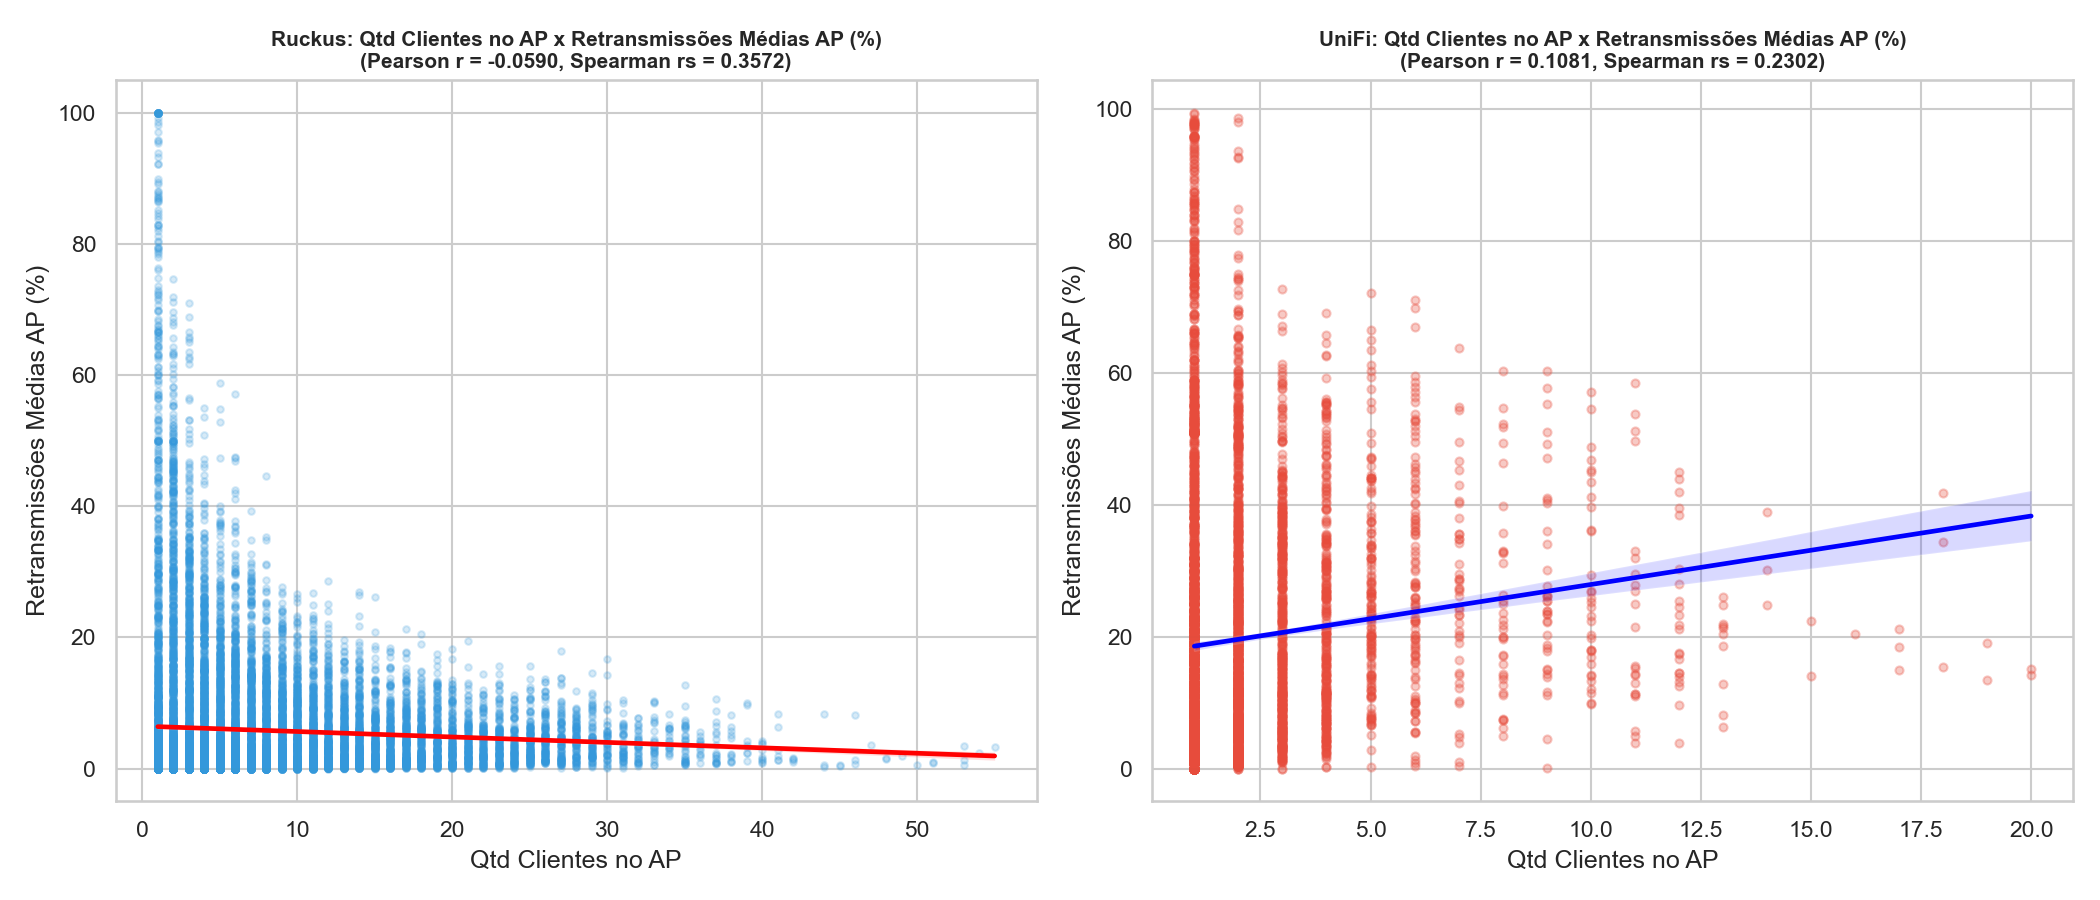
\includegraphics[width=0.85\textwidth]{img/05_clientes_retransmissoes_ap.png}
  \caption{Clientes x Retransmissões AP}
  \label{fig:05_clientes_retransmissoes_ap_png}
\end{figure}
\begin{itemize}
  \item \textbf{Expectativa Teórica}: Esperava-se uma correlação positiva moderada, dado que mais clientes compartilhando o canal físico via protocolo CSMA/CA aumentam as chances de colisão no ar.
  \item \textbf{Comportamento Observado}: Os dados mostram correlação nula no Ruckus (\textit{r\_p} = -0.0590, \textit{r\_s} = 0.3572) e muito fraca na UniFi (\textit{r\_p} = 0.1081, \textit{r\_s} = 0.2302).
  \item \textbf{Discussão}: Os coeficientes sugerem que os APs de ambas as marcas conseguem lidar satisfatoriamente com a coordenação de pacotes dos clientes e evitar colisões críticas sob as cargas observadas durante a coleta.
\end{itemize}

\subsubsection{Ruído de Fundo (Noise) × Retransmissões}
\begin{itemize}
  \item \textbf{Arquivo}: `06\_noise\_retransmissoes.png`
  \item \textbf{Visualização}:
\end{itemize}
\begin{figure}[H]
  \centering
  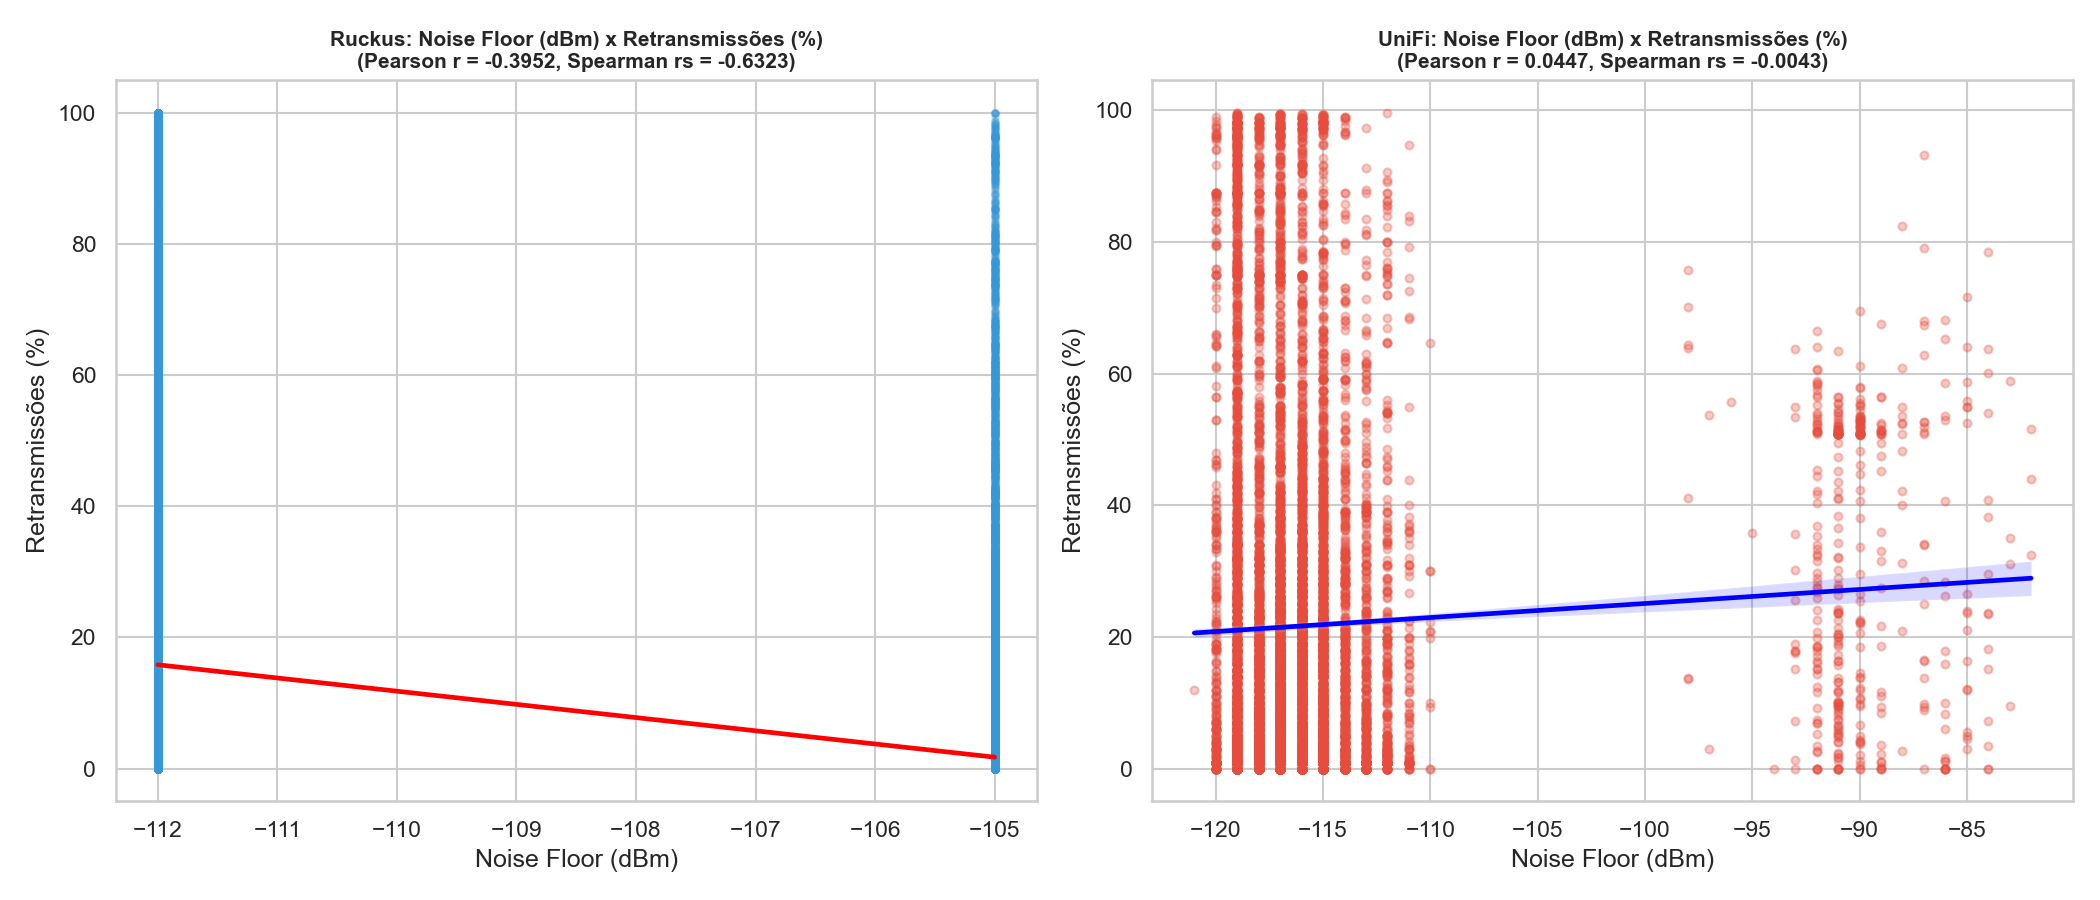
\includegraphics[width=0.85\textwidth]{img/06_noise_retransmissoes.png}
  \caption{Noise x Retransmissões}
  \label{fig:06_noise_retransmissoes_png}
\end{figure}
\begin{itemize}
  \item \textbf{Expectativa Teórica}: Esperava-se correlação positiva, uma vez que níveis de ruído elevados deterioram o SNR e a integridade física dos bits transmitidos.
  \item \textbf{Comportamento Observado}: Correlação nula no Ruckus (\textit{r\_p} = -0.3952, \textit{r\_s} = -0.6323) e na UniFi (\textit{r\_p} = 0.0447, \textit{r\_s} = -0.0043).
  \item \textbf{Discussão}: Isso sugere que o ruído ambiental no campus permaneceu em patamares baixos e estáveis (sem picos severos de interferência externa), não afetando de forma mensurável a estabilidade de pacotes nas conexões dos clientes.
\end{itemize}

\subsubsection{Ruído de Fundo (Noise) × RSSI}
\begin{itemize}
  \item \textbf{Arquivo}: `07\_noise\_rssi.png`
  \item \textbf{Visualização}:
\end{itemize}
\begin{figure}[H]
  \centering
  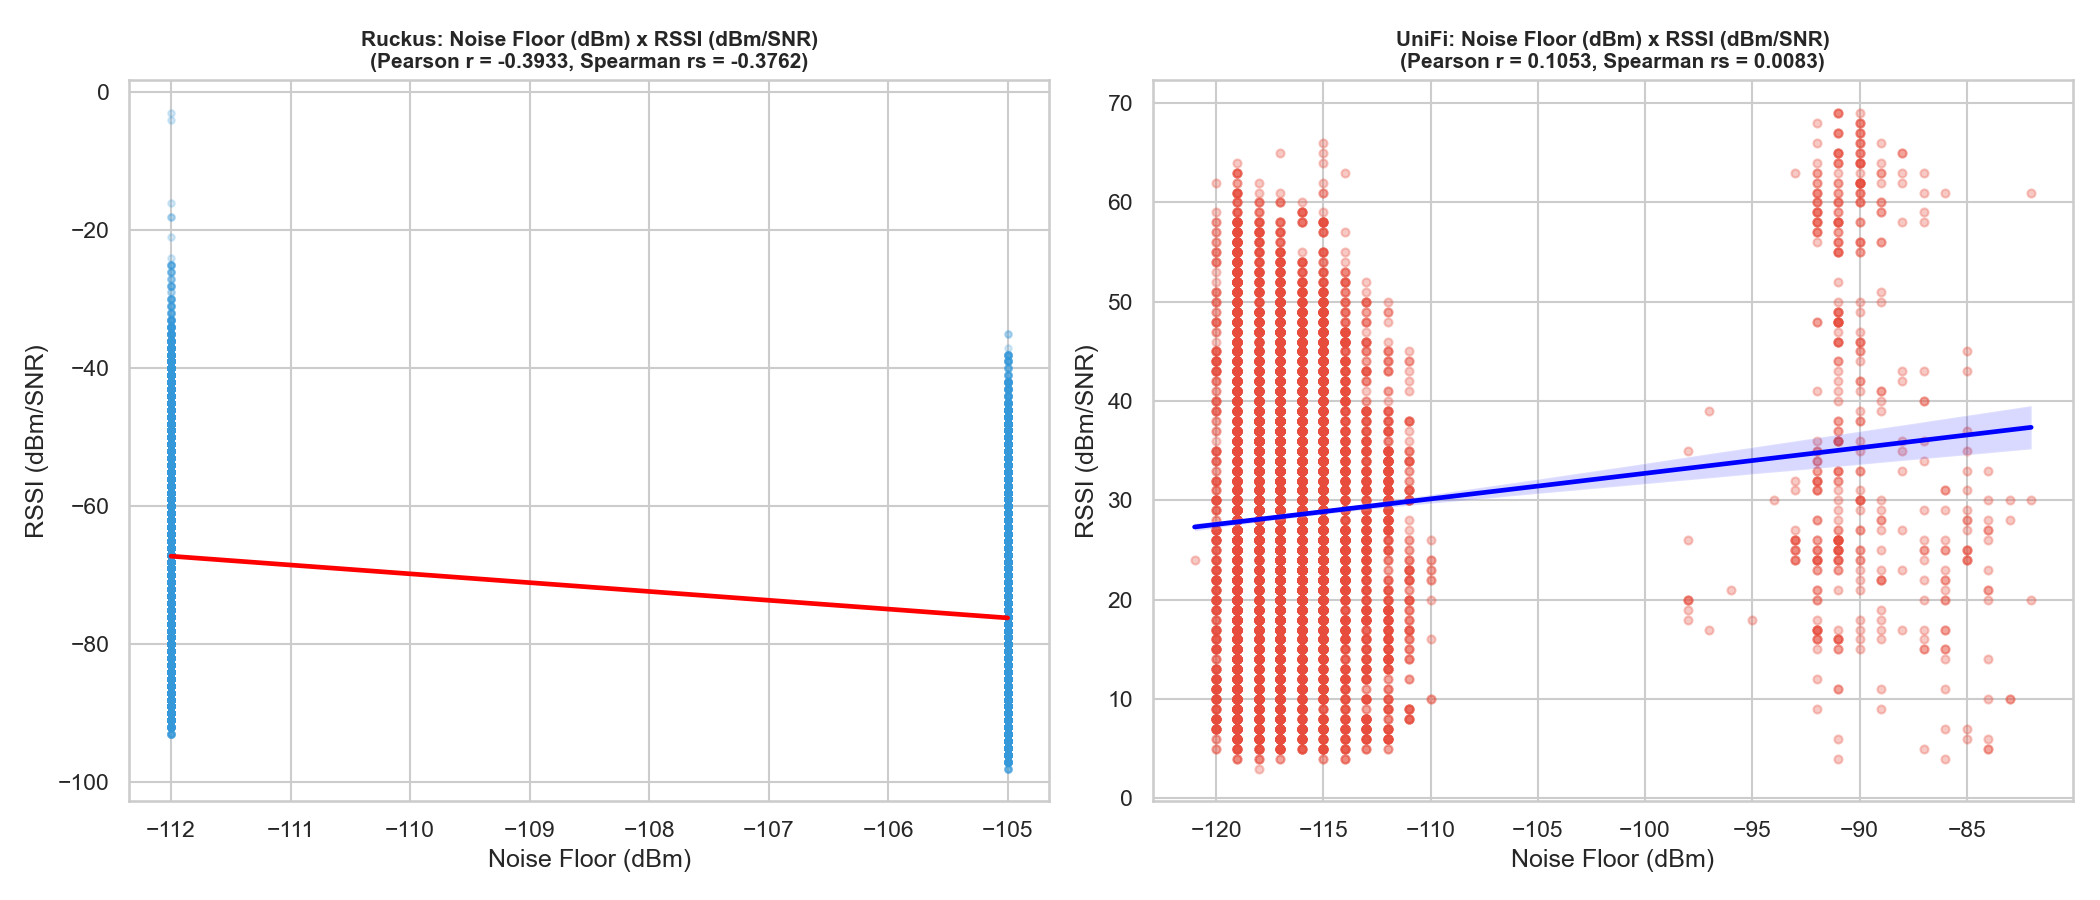
\includegraphics[width=0.85\textwidth]{img/07_noise_rssi.png}
  \caption{Noise x RSSI}
  \label{fig:07_noise_rssi_png}
\end{figure}
\begin{itemize}
  \item \textbf{Expectativa Teórica}: Esperava-se correlação nula. Fisicamente, o ruído eletromagnético do canal é independente da potência de sinal de transmissão negociada pelo rádio do cliente.
  \item \textbf{Comportamento Observado}: Correlação nula na UniFi (\textit{r\_p} = 0.1053, \textit{r\_s} = 0.0083), mas muito forte na Ruckus (\textit{r\_p} = -0.3933, \textit{r\_s} = -0.3762).
  \item \textbf{Discussão}: O resultado da UniFi apóia a física do canal de rádio. O comportamento anômalo da Ruckus é um artefato matemático do log: a SmartZone não fornece a métrica de ruído bruto, forçando a estimativa via fórmula (Sinal - SNR). Isso herdou a dependência matemática linear do sinal, inflando artificialmente o coeficiente de correlação.
\end{itemize}

\subsubsection{Link Speed TX × Throughput TX}
\begin{itemize}
  \item \textbf{Arquivo}: `08\_link\_speed\_throughput.png`
  \item \textbf{Visualização}:
\end{itemize}
\begin{figure}[H]
  \centering
  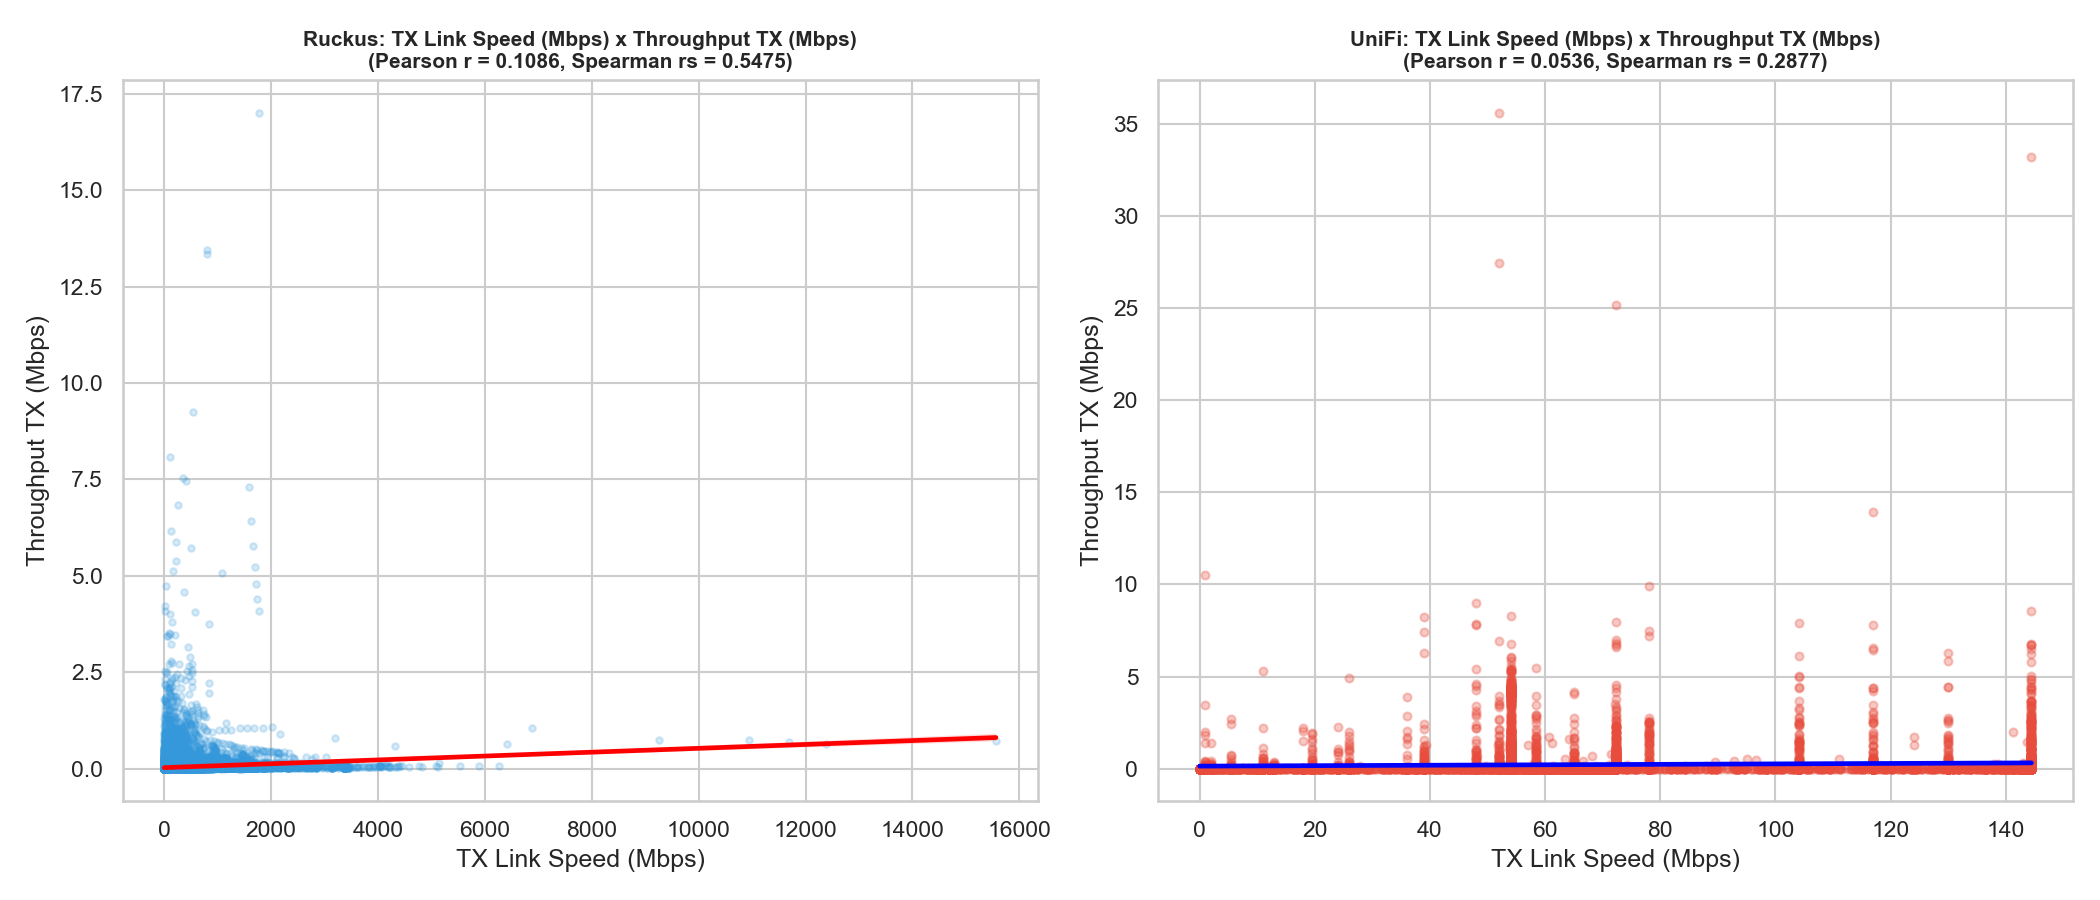
\includegraphics[width=0.85\textwidth]{img/08_link_speed_throughput.png}
  \caption{Link Speed x Throughput}
  \label{fig:08_link_speed_throughput_png}
\end{figure}
\begin{itemize}
  \item \textbf{Expectativa Teórica}: Esperava-se uma correlação positiva moderada. Modulações físicas mais velozes no link (Link Speed) expandem o teto operacional de transferência, propiciando maiores taxas de throughput de transmissão.
  \item \textbf{Comportamento Observado}: Correlação fraca no Ruckus (\textit{r\_p} = 0.1086, \textit{r\_s} = 0.5475) e nula na UniFi (\textit{r\_p} = 0.0536, \textit{r\_s} = 0.2877).
  \item \textbf{Discussão}: Esse resultado indica que a modulação de velocidade do link de rádio é mantida elevada pela proximidade física, porém a vazão real consumida depende exclusivamente do perfil e uso de aplicativos pelo cliente.
\end{itemize}

\subsubsection{Volume de Dados × Tempo de Sessão (Uptime)}
\begin{itemize}
  \item \textbf{Arquivo}: `09\_ruckus\_uptime\_volume.png`
  \item \textbf{Visualização}:
\end{itemize}
\begin{figure}[H]
  \centering
  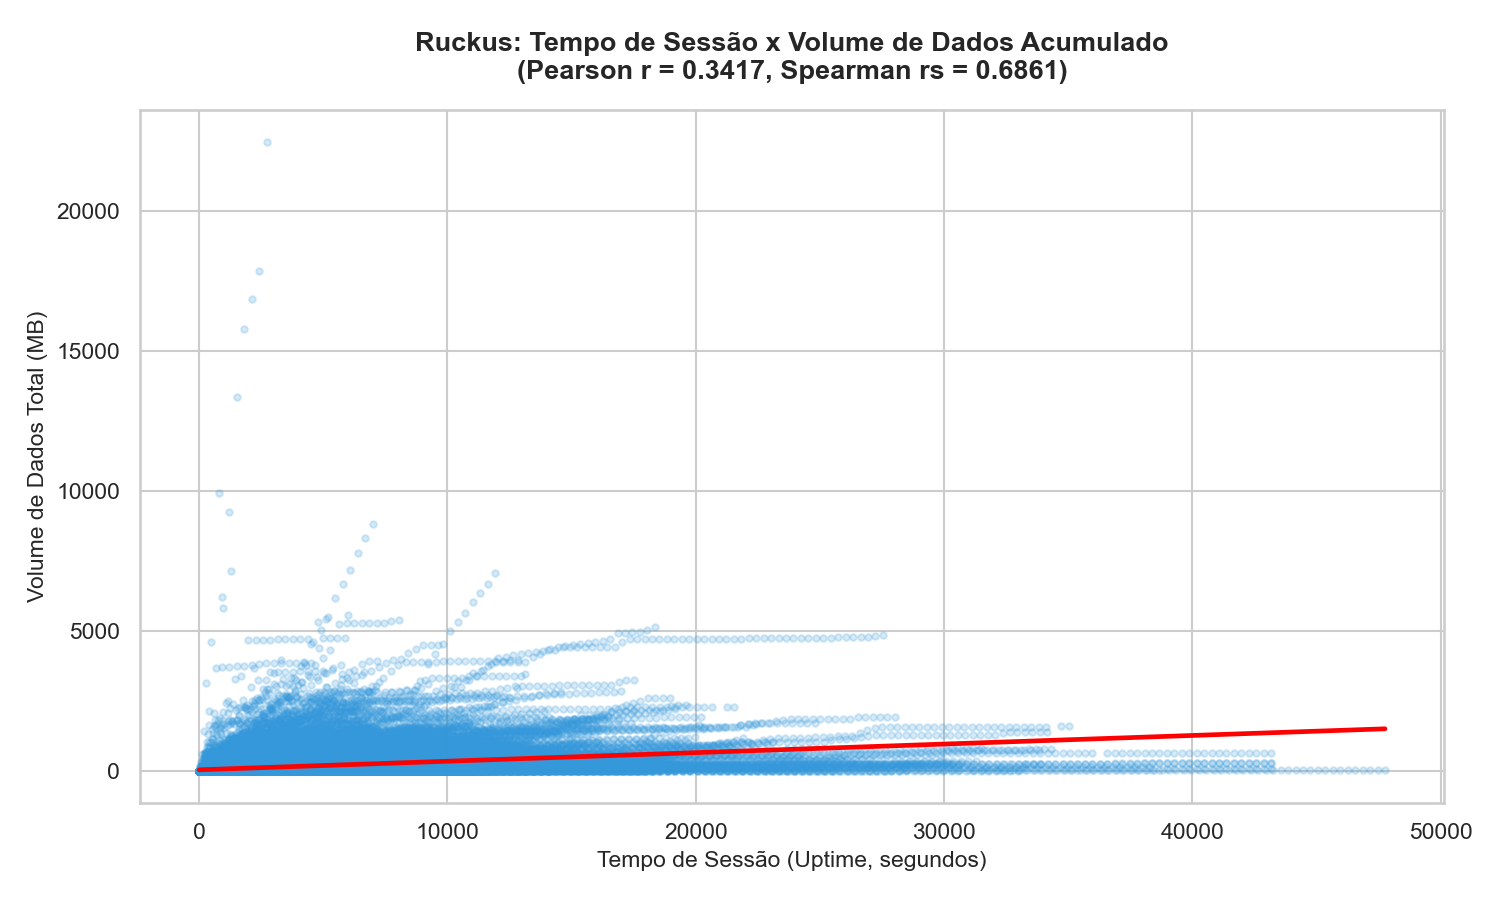
\includegraphics[width=0.85\textwidth]{img/09_ruckus_uptime_volume.png}
  \caption{Tempo de Sessão x Volume Ruckus}
  \label{fig:09_ruckus_uptime_volume_png}
\end{figure}
\begin{itemize}
  \item \textbf{Expectativa Teórica}: Esperava-se uma correlação positiva moderada a forte, dado que sessões de conexão mais duradouras propiciam o acúmulo integrado de mais bytes trafegados.
  \item \textbf{Comportamento Observado}: Correlação positiva moderada a forte no Ruckus (\textit{r\_p} = 0.3417, \textit{r\_s} = 0.6861) e na UniFi (\textit{r\_p} = 0.0980, \textit{r\_s} = 0.3121).
  \item \textbf{Discussão}: Os dados são consistentes com a teoria de rede. Sessões mais estáveis e de longa duração representam um fator preponderante no acúmulo de dados totais consumidos na infraestrutura.
\end{itemize}


\section{Testes Estatísticos de Hipótese}

\begin{itemize}
  \item \textbf{Limitação do Dataset da UniFi}:
    O conjunto de dados brutos da UniFi contém \textbf{apenas conexões ativas na banda de 2,4 GHz} ($N = 51974$). Não foram registradas coletas de clientes na banda de 5 GHz. Consequentemente, o teste comparativo de bandas (2,4 GHz vs 5 GHz) para a \textbf{UniFi} foi omitido por falta de amostras de 5 GHz, e a comparação de fabricantes em \textbf{5 GHz} foi classificada como \textit{Dados Insuficientes} e omitida das visualizações correspondentes.


\end{itemize}
\subsection{Metodologia Aplicada}

\begin{enumerate}
  \item \textbf{Verificação de Normalidade}:
  \begin{itemize}
    \item Utilizou-se o teste de \textbf{Shapiro-Wilk} (\texttt{scipy.stats.shapiro}).
    \item Devido ao tamanho elevado das amostras ($N = 446060$ no Ruckus e $N = 51974$ na UniFi), aplicou-se uma amostragem aleatória uniforme de 5,000 pontos para realizar o teste de forma válida (já que o teste é limitado a $N \le 5,000$).
    \item \textbf{Resultado Geral}: Para todas as métricas analisadas (Retransmissões, RSSI/Sinal e Throughput), a hipótese nula de normalidade foi \textbf{rejeitada} ($p < 0,001$, indicando que as amostras \textbf{não} seguem uma distribuição normal).
\end{itemize}
  \item \textbf{Escolha do Teste de Hipótese}:
  \begin{itemize}
    \item Como as amostras são não-normais, aplicou-se o teste não-paramétrico \textbf{U de Mann-Whitney} (\texttt{scipy.stats.mannwhitneyu}) para comparar as distribuições de dois grupos independentes (nível de significância alpha = 0,05).
\end{itemize}
  \item \textbf{Tamanho do Efeito (Effect Size)}:
  \begin{itemize}
    \item Para o teste U de Mann-Whitney, calculou-se o tamanho de efeito baseado no coeficiente de correlação de rank da distribuição normal padrão aproximada: \textit{r} = |Z| / sqrt(N).
    \item Critérios de magnitude para \textit{r}: |\textit{r}| >= 0,1 indica efeito pequeno; |\textit{r}| >= 0,3 efeito médio; |\textit{r}| >= 0,5 efeito grande.
    \item Para o Teste t de Welch (se aplicável), calculou-se o Cohen's d: |\textit{d}| >= 0,2 pequeno; |\textit{d}| >= 0,5 médio; |\textit{d}| >= 0,8 grande.


\end{itemize}
\end{enumerate}
\subsection{Tabela Consolidada de Testes de Hipótese}

\begin{table}[H]
\IBGEtab{%
  \caption{Tabela Consolidada de Testes de Hipótese}%
  \label{tab:data_testes_hipotese_1}%
}{%
  \centering\footnotesize
  \resizebox{\textwidth}{!}{%
    \begin{tabular}{lcccccc}
      Métrica & Comparação (A vs B) & Amostras (N\_A vs N\_B) & Média/Mediana (A vs B) & P-valor & Tam. Efeito (r / d) & Signif.? \\
      \midrule
      \textbf{RSSI} & RK 2,4G vs RK 5G & 103.050 vs 297.930 & -67,3/-67,0 vs -76,0/-77,0 & $p < 0,001$ (\textsuperscript{***}) & 0,3619 & \textbf{Sim} \\
      \textbf{Retransmissões} & RK 2,4G vs RK 5G & 118.225 vs 327.835 & 15,7/3,6 vs 2,0/0,0 & $p < 0,001$ (\textsuperscript{***}) & 0,5221 & \textbf{Sim} \\
      \textbf{Throughput} & RK 2,4G vs RK 5G & 118.225 vs 327.835 & 0,3/0,1 vs 0,5/0,2 & $p < 0,001$ (\textsuperscript{***}) & 0,1634 & \textbf{Sim} \\
      \textbf{RSSI} & UF 2,4G vs UF 5G & 51.974 vs 0 & N/A & N/A & N/A & \textbf{Insuf.} \\
      \textbf{Retransmissões} & UF 2,4G vs UF 5G & 51.974 vs 0 & N/A & N/A & N/A & \textbf{Insuf.} \\
      \textbf{Throughput} & UF 2,4G vs UF 5G & 51.974 vs 0 & N/A & N/A & N/A & \textbf{Insuf.} \\
      \textbf{Sinal Físico (dBm)} & Ruckus vs UniFi & 400.980 vs 51.974 & -73,8/-75,0 vs -66,2/-67,0 & $p < 0,001$ (\textsuperscript{***}) & 0,1870 & \textbf{Sim} \\
      \textbf{Retransmissões} & Ruckus vs UniFi & 446.060 vs 51.974 & 5,6/0,0 vs 21,7/12,3 & $p < 0,001$ (\textsuperscript{***}) & 0,3613 & \textbf{Sim} \\
      \textbf{Throughput} & Ruckus vs UniFi & 446.060 vs 51.974 & 0,5/0,1 vs 0,3/0,0 & $p < 0,001$ (\textsuperscript{***}) & 0,3332 & \textbf{Sim} \\
      \textbf{Índice de Equidade (Jain)} & Ruckus vs UniFi & 5.479 vs 3.181 & 0,3/0,3 vs 0,2/0,1 & $p < 0,001$ (\textsuperscript{***}) & 0,4484 & \textbf{Sim} \\
      \textbf{Sinal Físico (dBm)} & RK 2,4G vs UF 2,4G & 103.050 vs 51.974 & -67,3/-67,0 vs -66,2/-67,0 & $p < 0,001$ (\textsuperscript{***}) & 0,0300 & \textbf{Sim} \\
      \textbf{Retransmissões} & RK 2,4G vs UF 2,4G & 118.225 vs 51.974 & 15,7/3,6 vs 21,7/12,3 & $p < 0,001$ (\textsuperscript{***}) & 0,2101 & \textbf{Sim} \\
      \textbf{Throughput} & RK 2,4G vs UF 2,4G & 118.225 vs 51.974 & 0,3/0,1 vs 0,3/0,0 & $p < 0,001$ (\textsuperscript{***}) & 0,4441 & \textbf{Sim} \\
      \textbf{Sinal Físico (dBm)} & RK 5G vs UF 5G & 297.930 vs 0 & N/A & N/A & N/A & \textbf{Insuf.} \\
      \textbf{Retransmissões} & RK 5G vs UF 5G & 327.835 vs 0 & N/A & N/A & N/A & \textbf{Insuf.} \\
      \textbf{Throughput} & RK 5G vs UF 5G & 327.835 vs 0 & N/A & N/A & N/A & \textbf{Insuf.} \\
      \bottomrule
    \end{tabular}%
  }%
}{%
  \fonte{Produzido pelos autores.}%
}
\end{table}

\textit{Nota sobre a Tabela Consolidada}: Os resultados sugerem diferenças estatisticamente significativas para todas as métricas comparadas que dispõem de dados suficientes ($p < 0,05$). Os coeficientes de tamanho de efeito (\textit{r}) indicam magnitudes variadas, sugerindo que os desvios mais proeminentes localizam-se nas taxas de retransmissão e nas potências de sinal entre bandas, enquanto as diferenças de throughput sustentado e equidade apresentam efeitos sob a ótica amostral deste ambiente específico.

Em termos práticos de rede, essas diferenças observadas sugerem as seguintes implicações:
\begin{enumerate}
  \item \textbf{RSSI e Cobertura Física}: A atenuação mais acentuada verificada na banda de 5 GHz (RSSI inferior no Ruckus) pode implicar em células de cobertura menores, sugerindo a necessidade de um planejamento de posicionamento de APs mais denso para evitar áreas de sombra. No entanto, onde há boa intensidade de sinal, a menor interferência dessa banda tende a favorecer taxas de modulação superiores.
  \item \textbf{Eficiência de Airtime (Retransmissões)}: O maior índice médio de retransmissões associado à UniFi sugere que o tempo de uso do canal de rádio ("airtime") pode estar sendo mais consumido por repetições de quadros do que na Ruckus. Na prática, retransmissões mais elevadas reduzem a eficiência geral do canal, podendo degradar o tempo de resposta em ambientes muito povoados.
  \item \textbf{Vazão Percebida (Throughput)}: A vazão individual média superior identificada no Ruckus sugere que os clientes ativos nessa rede obtiveram uma experiência potencialmente mais ágil no escoamento de dados. Contudo, dado que o throughput médio em ambas as redes permaneceu abaixo de 1 Mbps, isso indica que a maioria dos dispositivos esteve em estado ocioso ou consumindo serviços de baixa demanda.
  \item \textbf{Índice de Equidade (Jain)}: A comparação do índice de equidade de Jain entre os fabricantes revela se a distribuição de throughput foi estatisticamente mais equilibrada em uma das marcas. Uma diferença significativa indica que os algoritmos de gerenciamento de RF e compartilhamento de canal de um dos fabricantes operaram de forma mais justa no cenário observado.


\end{enumerate}
\subsection{Discussão Detalhada das Comparações}

\subsubsection{Comparação de Bandas (2,4 GHz vs 5 GHz)}

\paragraph{Ruckus}
\begin{itemize}
  \item \textbf{Visualização}:
\end{itemize}
\begin{figure}[H]
  \centering
  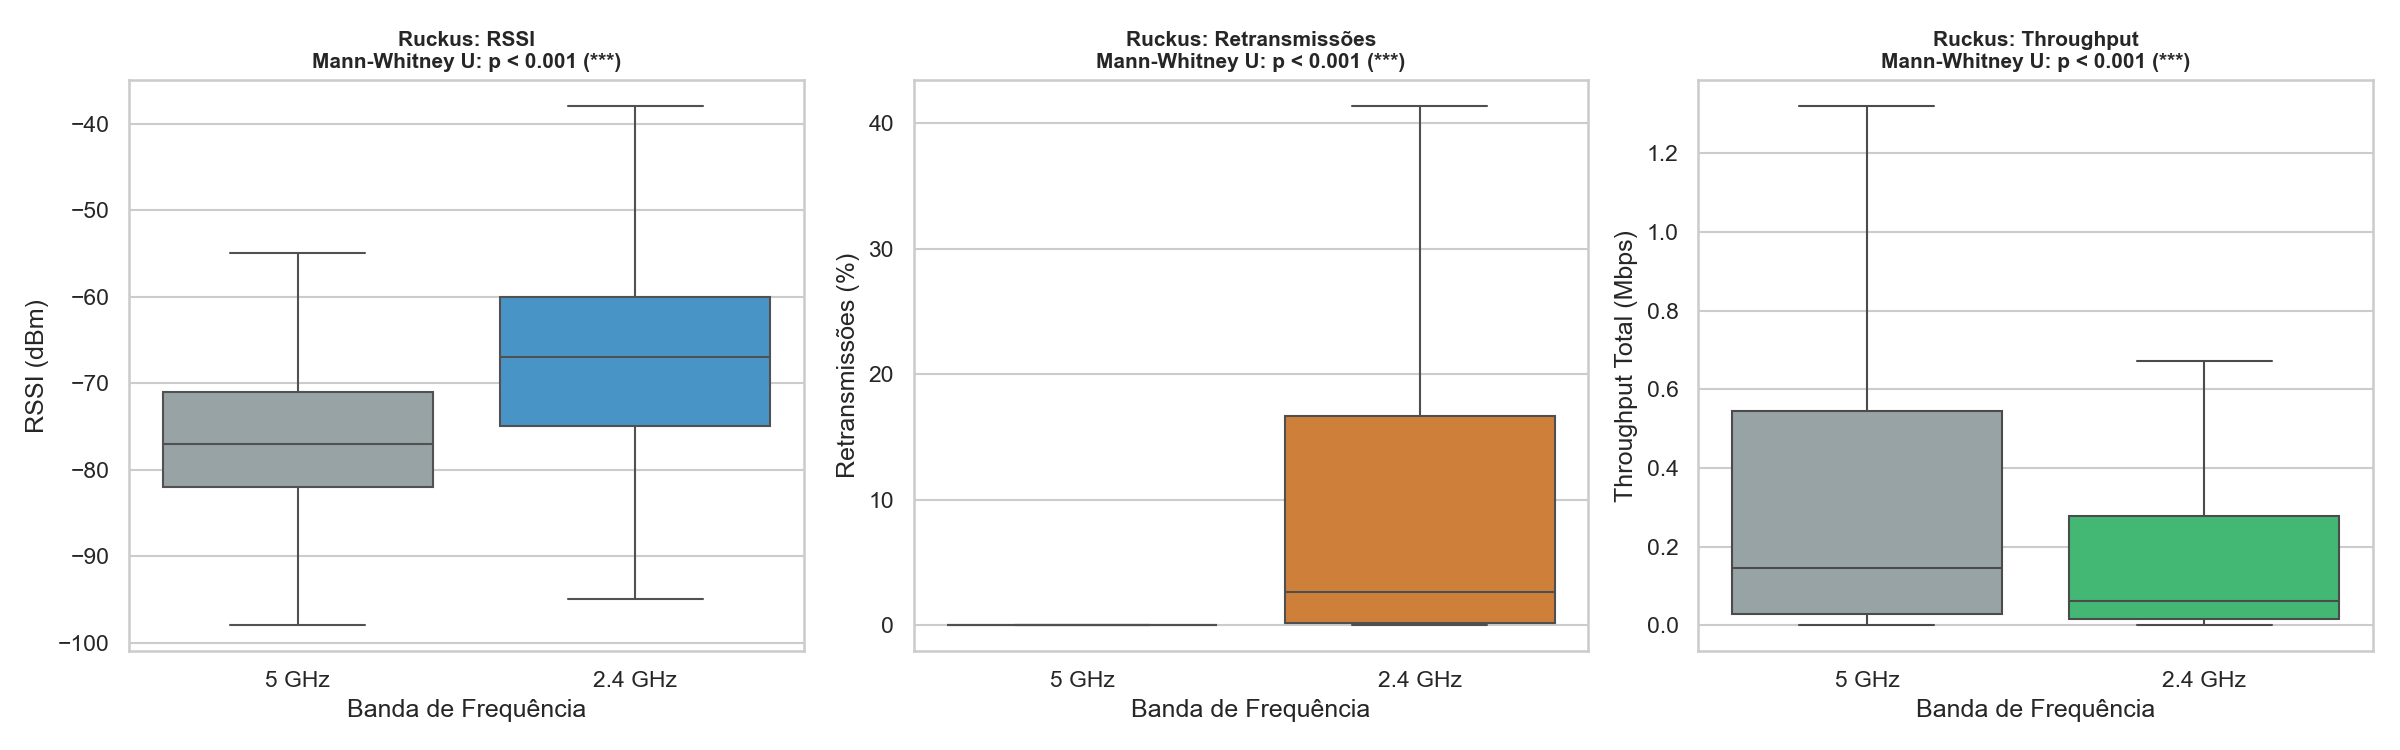
\includegraphics[width=0.85\textwidth]{img/01_ruckus_bandas_comparacao.png}
  \caption{Comparação de Bandas Ruckus}
  \label{fig:01_ruckus_bandas_comparacao_png}
\end{figure}
\begin{itemize}
  \item \textbf{RSSI}: A diferença é altamente significativa ($p < 0,001$) com tamanho de efeito médio (\textit{r} = 0,3619). A mediana em 2,4 GHz é de \texttt{-67.0 dBm} contra \texttt{-77.0 dBm} em 5 GHz, refletindo a física de atenuação do sinal de 5 GHz.
  \item \textbf{Retransmissões}: Diferença estatisticamente significativa ($p < 0,001$) com tamanho de efeito grande (\textit{r} = 0,5221). O 2,4 GHz possui retransmissões médias de \texttt{15.71\%} contra \texttt{1.98\%} do 5 GHz, condizente com a poluição de espectro na frequência mais baixa.
  \item \textbf{Throughput}: Diferença estatisticamente significativa ($p < 0,001$) com tamanho de efeito pequeno (\textit{r} = 0,1634). O throughput médio em 5 GHz (\texttt{0.545 Mbps}) mostra-se superior ao de 2,4 GHz (\texttt{0.257 Mbps}).

  \item \textbf{UniFi}: Omitido devido à indisponibilidade de conexões em 5 GHz na telemetria da UniFi.


\end{itemize}
\subsubsection{Comparação de Fabricantes (Ruckus vs UniFi)}

\paragraph{Geral}
\begin{itemize}
  \item \textbf{Visualização}:
\end{itemize}
\begin{figure}[H]
  \centering
  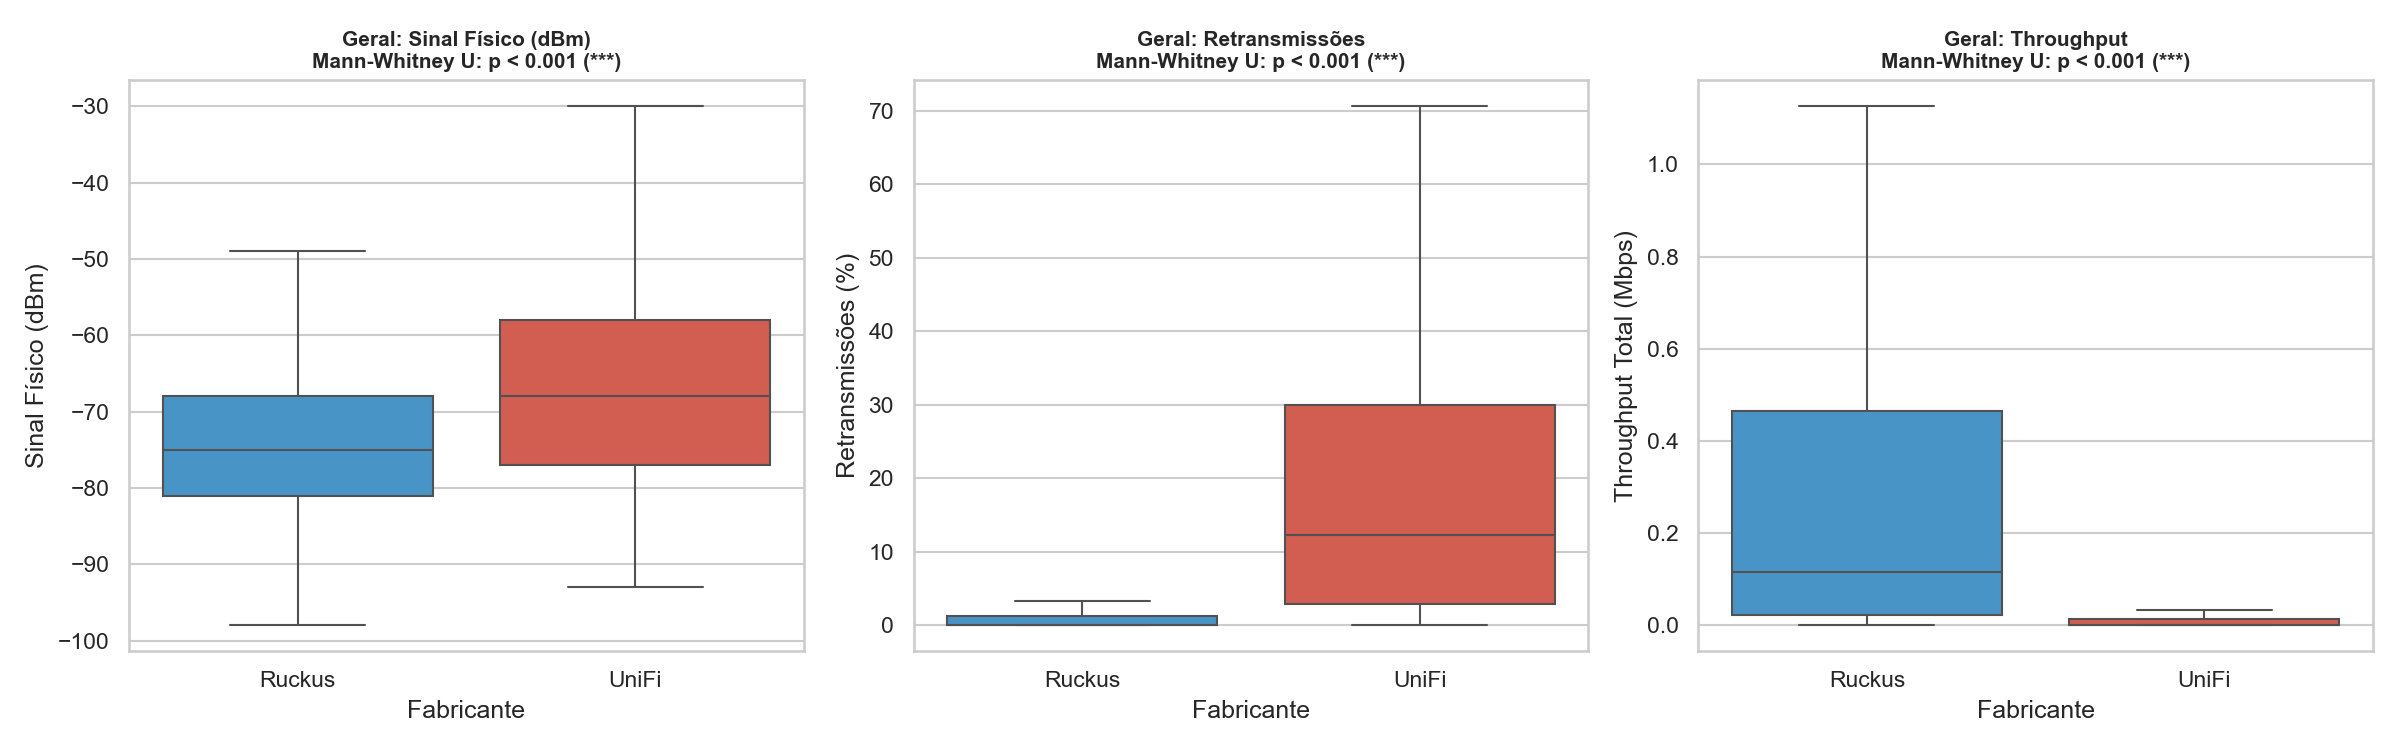
\includegraphics[width=0.85\textwidth]{img/03_fabricantes_geral_comparacao.png}
  \caption{Comparação de Fabricantes Geral}
  \label{fig:03_fabricantes_geral_comparacao_png}
\end{figure}
\begin{itemize}
  \item \textbf{Sinal Físico (dBm)}: A UniFi registrou mediana de sinal físico de \texttt{-67.0 dBm} enquanto a Ruckus registrou \texttt{-75.0 dBm}, diferença significativa ($p < 0,001$) com tamanho de efeito pequeno (\textit{r} = 0,1870). Isso reflete as características físicas específicas dos locais monitorados (escritórios e laboratórios com menor distância média aos APs na UniFi), embora a intensidade do sinal dependa também das antenas, potência de transmissão e características de hardware dos dispositivos clientes.
  \item \textbf{Retransmissões}: A diferença é altamente significativa ($p < 0,001$) com tamanho de efeito médio (\textit{r} = 0,3613). A UniFi apresenta média de \texttt{21.65\%} contra \texttt{5.62\%} do Ruckus. Esta disparidade indica a influência da metodologia de medição: a UniFi estima a retransmissão indiretamente com base no CCQ do firmware, enquanto a Ruckus monitora estritamente a taxa de quadros físicos retransmitidos no rádio.
  \item \textbf{Throughput}: A Ruckus registrou throughput médio de \texttt{0.469 Mbps} contra \texttt{0.257 Mbps} da UniFi, com diferença estatisticamente significativa ($p < 0,001$) e tamanho de efeito médio (\textit{r} = 0,3332). Os resultados sugerem que a rede Ruckus escoou uma taxa superior de dados por cliente no cenário coletado.
  \item \textbf{Índice de Equidade (Jain)}: A comparação da equidade de compartilhamento de throughput entre os clientes conectados simultaneamente revelou diferença estatisticamente significativa ($p < 0,001$) com tamanho de efeito médio (\textit{r} = 0,4484). A Ruckus registrou equidade média de \texttt{0.3427} e mediana de \texttt{0.2637}, enquanto a UniFi obteve média de \texttt{0.1904} e mediana de \texttt{0.1378}. Isso sugere tendências distintas no balanceamento de carga entre os clientes ativos de cada fabricante.

\end{itemize}
\paragraph{Comparações por Banda de 2,4 GHz (Isolado)}
\begin{itemize}
  \item \textbf{Visualização 2,4 GHz}:
\end{itemize}
\begin{figure}[H]
  \centering
  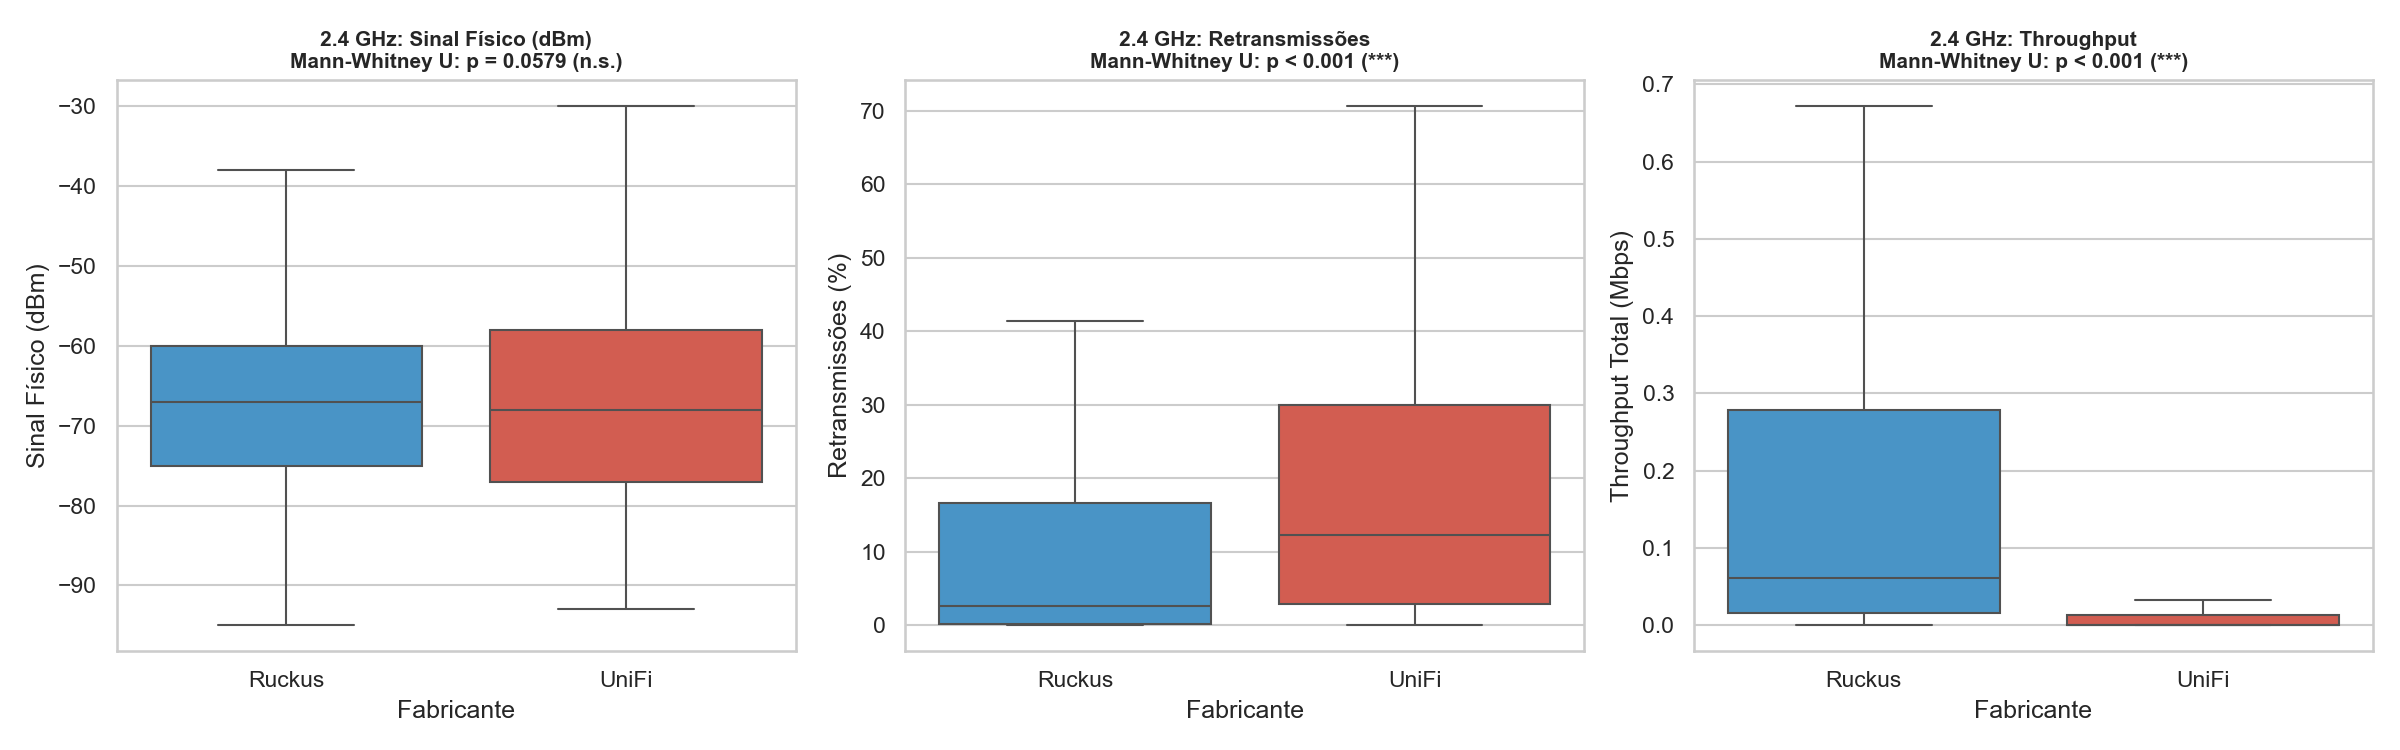
\includegraphics[width=0.85\textwidth]{img/04_fabricantes_24ghz_comparacao.png}
  \caption{Comparação de Fabricantes 2.4 GHz}
  \label{fig:04_fabricantes_24ghz_comparacao_png}
\end{figure}
\begin{itemize}
  \item As tendências observadas no cenário geral se mantêm na frequência isolada de 2,4 GHz: o sinal recebido na UniFi apresenta-se melhor ($p < 0,001$), o throughput médio na Ruckus é superior ($p < 0,001$) e a taxa de retransmissões baseada no CCQ na UniFi mostra-se consideravelmente maior ($p < 0,001$).

\end{itemize}
\paragraph{Comparações por Banda de 5 GHz (Isolado)}
\begin{itemize}
  \item \textit{Nota}: Não é possível realizar a comparação em 5 GHz entre fabricantes, pois a UniFi não registrou telemetria nessa frequência.


\end{itemize}
\subsection{Tabela Detalhada dos Testes de Hipótese}

A tabela abaixo apresenta os mesmos testes estatísticos em formato expandido, contendo os resultados individuais de verificação de normalidade (Shapiro-Wilk), o tipo de teste selecionado (U de Mann-Whitney ou Teste t) e o valor bruto calculado da estatística de teste.

\begin{table}[H]
\IBGEtab{%
  \caption{Tabela Detalhada dos Testes de Hipótese}%
  \label{tab:data_testes_hipotese_2}%
}{%
  \centering\footnotesize
  \resizebox{\textwidth}{!}{%
    \begin{tabular}{lcccccccccc}
      Métrica & Grupo A & Grupo B & Média/Mediana A & Média/Mediana B & Normal A/B & Teste Aplicado & Estatística & P-valor & Tam. Efeito (r / d) & Diferença Significativa? \\
      \midrule
      \textbf{RSSI} & Ruckus 2,4G & Ruckus 5G & -67,304 / -67,000 & -75,984 / -77,000 & Não/Não & Mann-Whitney U & 22691746053,50 & $p < 0,001$ (\textsuperscript{***}) & 0,3619 & \textbf{Sim} \\
      \textbf{Retransmissões} & Ruckus 2,4G & Ruckus 5G & 15,706 / 3,641 & 1,983 / 0,000 & Não/Não & Mann-Whitney U & 32613638143,50 & $p < 0,001$ (\textsuperscript{***}) & 0,5221 & \textbf{Sim} \\
      \textbf{Throughput} & Ruckus 2,4G & Ruckus 5G & 0,257 / 0,060 & 0,545 / 0,150 & Não/Não & Mann-Whitney U & 15236405525,50 & $p < 0,001$ (\textsuperscript{***}) & 0,1634 & \textbf{Sim} \\
      \textbf{RSSI} & UniFi 2,4G & UniFi 5G & 29,576 / 29,000 & N/A & N/A/N/A & Nenhum (Dados Insuficientes) & N/A & N/A & N/A & \textbf{Dados Insuficientes} \\
      \textbf{Retransmissões} & UniFi 2,4G & UniFi 5G & 21,654 / 12,300 & N/A & N/A/N/A & Nenhum (Dados Insuficientes) & N/A & N/A & N/A & \textbf{Dados Insuficientes} \\
      \textbf{Throughput} & UniFi 2,4G & UniFi 5G & 0,257 / 0,000 & N/A & N/A/N/A & Nenhum (Dados Insuficientes) & N/A & N/A & N/A & \textbf{Dados Insuficientes} \\
      \textbf{Sinal Físico (dBm)} & Ruckus & UniFi & -73,753 / -75,000 & -66,223 / -67,000 & Não/Não & Mann-Whitney U & 6889907166,50 & $p < 0,001$ (\textsuperscript{***}) & 0,1870 & \textbf{Sim} \\
      \textbf{Retransmissões} & Ruckus & UniFi & 5,620 / 0,000 & 21,654 / 12,300 & Não/Não & Mann-Whitney U & 3682452798,00 & $p < 0,001$ (\textsuperscript{***}) & 0,3613 & \textbf{Sim} \\
      \textbf{Throughput} & Ruckus & UniFi & 0,469 / 0,116 & 0,257 / 0,000 & Não/Não & Mann-Whitney U & 18886445094,50 & $p < 0,001$ (\textsuperscript{***}) & 0,3332 & \textbf{Sim} \\
      \textbf{Índice de Equidade (Jain)} & Ruckus & UniFi & 0,343 / 0,264 & 0,190 / 0,138 & Não/Não & Mann-Whitney U & 13393982,00 & $p < 0,001$ (\textsuperscript{***}) & 0,4484 & \textbf{Sim} \\
      \textbf{Sinal Físico (dBm)} & Ruckus 2,4G & UniFi 2,4G & -67,304 / -67,000 & -66,223 / -67,000 & Não/Não & Mann-Whitney U & 2579762545,50 & $p < 0,001$ (\textsuperscript{***}) & 0,0300 & \textbf{Sim} \\
      \textbf{Retransmissões} & Ruckus 2,4G & UniFi 2,4G & 15,706 / 3,641 & 21,654 / 12,300 & Não/Não & Mann-Whitney U & 2263260611,50 & $p < 0,001$ (\textsuperscript{***}) & 0,2101 & \textbf{Sim} \\
      \textbf{Throughput} & Ruckus 2,4G & UniFi 2,4G & 0,257 / 0,060 & 0,257 / 0,000 & Não/Não & Mann-Whitney U & 4782877481,00 & $p < 0,001$ (\textsuperscript{***}) & 0,4441 & \textbf{Sim} \\
      \textbf{Sinal Físico (dBm)} & Ruckus 5G & UniFi 5G & -75,984 / -77,000 & N/A & N/A/N/A & Nenhum (Dados Insuficientes) & N/A & N/A & N/A & \textbf{Dados Insuficientes} \\
      \textbf{Retransmissões} & Ruckus 5G & UniFi 5G & 1,983 / 0,000 & N/A & N/A/N/A & Nenhum (Dados Insuficientes) & N/A & N/A & N/A & \textbf{Dados Insuficientes} \\
      \textbf{Throughput} & Ruckus 5G & UniFi 5G & 0,545 / 0,150 & N/A & N/A/N/A & Nenhum (Dados Insuficientes) & N/A & N/A & N/A & \textbf{Dados Insuficientes} \\
      \bottomrule
    \end{tabular}%
  }%
}{%
  \fonte{Produzido pelos autores.}%
}
\end{table}


\section{Classificação de Gargalos de Rede}

\subsection{Limiares de Decisão Estabelecidos}

\begin{enumerate}
  \item \textbf{G1: Baixa Qualidade de Enlace}: Potência física de sinal recebido pelo AP (\texttt{signal}) < \texttt{-75 dBm}.
  \item \textbf{G2: Congestionamento do Meio}: Número de clientes simultâneos conectados no mesmo AP e minuto >= 15.
  \item \textbf{G3: Interferência / SNR Ruim}: Ruído de fundo (\texttt{noise}) > \texttt{-90 dBm} ou SNR < \texttt{20 dB} em clientes com bom sinal (>= -75 dBm).
  \item \textbf{G4: Instabilidade de Roaming}: Clientes (MAC) que registraram > 5 trocas de AP no período de observação.
  \item \textbf{G5: Gargalo Cabeado (FE)}: Throughput de tráfego agregado sustentado do AP >= 90 Mbps (limite de interface Fast Ethernet de 100 Mbps).


\end{enumerate}
\subsection{Tabela Geral de Ocorrência e Impacto de Gargalos}

A Tabela Geral de Ocorrência apresenta as taxas e consequências físicas associadas a cada tipo de gargalo detectado de forma isolada ao longo do monitoramento de produção.

\begin{table}[H]
\IBGEtab{%
  \caption{Tabela Geral de Ocorrência e Impacto de Gargalos}%
  \label{tab:data_classificacao_gargalos_1}%
}{%
  \centering\footnotesize
  \resizebox{0.92\textwidth}{!}{%
    \begin{tabular}{lccccc}
      Fabricante & Categoria de Gargalo & Amostras (N) & Porcentagem (\%) & Throughput Cliente (Méd/Med) [Mbps] & Retransmissões (Méd/Med) [\%] \\
      \midrule
      \textbf{Ruckus} & G1: Baixa Qualidade de Enlace & 192.148 & 43,08\% & 0,502 / 0,129 & 5,37\% / 0,00\% \\
      \textbf{UniFi} & G1: Baixa Qualidade de Enlace & 13.663 & 26,29\% & 0,030 / 0,000 & 35,27\% / 25,00\% \\
      \textbf{Ruckus} & G2: Congestionamento do Meio & 198.696 & 44,54\% & 0,484 / 0,125 & 4,73\% / 0,00\% \\
      \textbf{UniFi} & G2: Congestionamento do Meio & 1.344 & 2,59\% & 0,227 / 0,002 & 22,50\% / 14,40\% \\
      \textbf{Ruckus} & G3: Interferência / SNR Ruim & 0 & 0,00\% & 0,000 / 0,000 & 0,00\% / 0,00\% \\
      \textbf{UniFi} & G3: Interferência / SNR Ruim & 544 & 1,05\% & 0,101 / 0,000 & 32,45\% / 30,90\% \\
      \textbf{Ruckus} & G4: Instabilidade de Roaming & 262.678 & 58,89\% & 0,397 / 0,109 & 6,39\% / 0,00\% \\
      \textbf{UniFi} & G4: Instabilidade de Roaming & 12.630 & 24,30\% & 0,180 / 0,000 & 17,10\% / 10,00\% \\
      \textbf{Ruckus} & G5: Gargalo Cabeado (FE) & 33 & 0,01\% & 6,219 / 0,144 & 2,11\% / 0,75\% \\
      \textbf{UniFi} & G5: Gargalo Cabeado (FE) & 0 & 0,00\% & 0,000 / 0,000 & 0,00\% / 0,00\% \\
      \textbf{Ruckus} & Sem Gargalos & 58.454 & 13,10\% & 0,493 / 0,100 & 4,49\% / 0,00\% \\
      \textbf{UniFi} & Sem Gargalos & 27.115 & 52,17\% & 0,384 / 0,001 & 17,39\% / 9,30\% \\
      \bottomrule
    \end{tabular}%
  }%
}{%
  \fonte{Produzido pelos autores.}%
}
\end{table}


\subsection{Análise de Desempenho e Carga por Access Point}

Abaixo são apresentados os perfis consolidados de carga e desempenho de cada Access Point mapeado na coleta, ordenados pelo throughput agregado médio (indicador de demanda atendida).

\subsubsection{Rede Ruckus (APs MAC Simplificados)}

\begin{table}[H]
\IBGEtab{%
  \caption{Rede Ruckus (APs MAC Simplificados)}%
  \label{tab:data_classificacao_gargalos_2}%
}{%
  \centering\footnotesize
  \resizebox{\textwidth}{!}{%
    \begin{tabular}{lcccccccc}
      Access Point & Amostras (N) & Clientes Médios (Pico) & Throughput Agregado Médio (Max) [Mbps] & Sinal Médio [dBm] & Retransmissões Médias [\%] & Throughput Médio p/ Cliente [Mbps] & Equidade Média (Jain) & Perfil Operacional (Cluster) \\
      \midrule
      \textbf{RK-fea0} & 38.146 & 22,7 (max 64) & 15,397 (max 111,108) & -75,7 & 3,75\% & 0,638 & 0,2935 & Grupo A: Muito Carregado \\
      \textbf{RK-0d40} & 35.809 & 20,6 (max 49) & 11,105 (max 54,074) & -75,6 & 4,05\% & 0,538 & 0,3067 & Grupo A: Muito Carregado \\
      \textbf{RK-2fd0} & 25.176 & 16,4 (max 42) & 8,284 (max 46,102) & -74,2 & 4,17\% & 0,520 & 0,3495 & Grupo C: Carga Moderada \\
      \textbf{RK-27d0} & 42.244 & 21,4 (max 55) & 8,205 (max 37,443) & -75,7 & 6,61\% & 0,390 & 0,3261 & Grupo C: Carga Moderada \\
      \textbf{RK-35c0} & 23.807 & 13,9 (max 36) & 8,074 (max 57,785) & -74,1 & 7,44\% & 0,565 & 0,3613 & Grupo C: Carga Moderada \\
      \textbf{RK-4050} & 29.173 & 17,1 (max 46) & 8,044 (max 32,117) & -72,5 & 5,27\% & 0,467 & 0,3457 & Grupo C: Carga Moderada \\
      \textbf{RK-efe0} & 30.711 & 14,0 (max 46) & 7,051 (max 56,451) & -65,9 & 4,39\% & 0,554 & 0,3868 & Grupo C: Carga Moderada \\
      \textbf{RK-51f0} & 38.558 & 17,3 (max 41) & 6,383 (max 47,167) & -74,7 & 5,98\% & 0,373 & 0,3636 & Grupo C: Carga Moderada \\
      \textbf{RK-9660} & 19.921 & 13,2 (max 35) & 5,786 (max 53,827) & -73,9 & 4,95\% & 0,456 & 0,3653 & Grupo C: Carga Moderada \\
      \textbf{RK-1e40} & 12.794 & 11,9 (max 39) & 5,416 (max 84,886) & -74,2 & 6,05\% & 0,458 & 0,4185 & Grupo C: Carga Moderada \\
      \textbf{RK-3180} & 20.228 & 13,1 (max 35) & 5,264 (max 53,483) & -74,6 & 3,92\% & 0,400 & 0,3985 & Grupo C: Carga Moderada \\
      \textbf{RK-1060} & 15.381 & 9,9 (max 26) & 4,367 (max 44,399) & -75,0 & 3,97\% & 0,457 & 0,3878 & Grupo C: Carga Moderada \\
      \textbf{RK-0780} & 1.483 & 15,7 (max 29) & 3,805 (max 17,069) & -69,5 & 4,04\% & 0,236 & 0,3267 & Grupo C: Carga Moderada \\
      \textbf{RK-42a0} & 11.694 & 7,4 (max 28) & 3,737 (max 34,312) & -70,8 & 4,36\% & 0,497 & 0,4808 & Grupo B: Pouco Utilizado \\
      \textbf{RK-7090} & 12.790 & 8,3 (max 25) & 3,667 (max 28,851) & -73,4 & 7,15\% & 0,413 & 0,4018 & Grupo B: Pouco Utilizado \\
      \textbf{RK-e8a0} & 15.959 & 10,5 (max 31) & 3,541 (max 61,206) & -72,4 & 5,35\% & 0,405 & 0,4056 & Grupo B: Pouco Utilizado \\
      \textbf{RK-1730} & 21.933 & 9,0 (max 26) & 3,479 (max 29,586) & -74,3 & 7,85\% & 0,465 & 0,4211 & Grupo D: Baixa Qualidade de Sinal \\
      \textbf{RK-3b10} & 7.700 & 6,9 (max 17) & 2,821 (max 40,003) & -72,7 & 5,77\% & 0,408 & 0,4933 & Grupo B: Pouco Utilizado \\
      \textbf{RK-1c10} & 9.343 & 6,5 (max 22) & 2,810 (max 31,876) & -75,0 & 9,32\% & 0,421 & 0,4769 & Grupo D: Baixa Qualidade de Sinal \\
      \textbf{RK-f3f0} & 9.861 & 4,1 (max 13) & 2,169 (max 47,419) & -71,2 & 7,16\% & 0,504 & 0,4853 & Grupo B: Pouco Utilizado \\
      \textbf{RK-5fe0} & 6.723 & 4,4 (max 12) & 1,977 (max 55,447) & -72,3 & 8,25\% & 0,422 & 0,5014 & Grupo B: Pouco Utilizado \\
      \textbf{RK-3440} & 11.513 & 8,9 (max 34) & 1,942 (max 26,487) & -77,0 & 11,41\% & 0,228 & 0,4037 & Grupo D: Baixa Qualidade de Sinal \\
      \textbf{RK-edd0} & 1.855 & 3,4 (max 8) & 1,807 (max 8,914) & -73,7 & 1,95\% & 0,567 & 0,5890 & Grupo B: Pouco Utilizado \\
      \textbf{RK-dcd0} & 3.258 & 4,7 (max 16) & 1,044 (max 8,827) & -74,7 & 7,27\% & 0,231 & 0,4471 & Grupo D: Baixa Qualidade de Sinal \\
      \bottomrule
    \end{tabular}%
  }%
}{%
  \fonte{Produzido pelos autores.}%
}
\end{table}

\subsubsection{Rede UniFi (APs Cadastrados)}

\begin{table}[H]
\IBGEtab{%
  \caption{Rede UniFi (APs Cadastrados)}%
  \label{tab:data_classificacao_gargalos_3}%
}{%
  \centering\footnotesize
  \resizebox{\textwidth}{!}{%
    \begin{tabular}{lcccccccc}
      Access Point & Amostras (N) & Clientes Médios (Pico) & Throughput Agregado Médio (Max) [Mbps] & Sinal Médio [dBm] & Retransmissões Médias [\%] & Throughput Médio p/ Cliente [Mbps] & Equidade Média (Jain) & Perfil Operacional (Cluster) \\
      \midrule
      \textbf{Lab Redes} & 8.894 & 7,7 (max 21) & 2,078 (max 44,247) & -67,0 & 23,29\% & 0,224 & 0,2861 & Grupo A: Muito Carregado \\
      \textbf{Guarita Entrada} & 9.280 & 4,8 (max 19) & 1,708 (max 14,370) & -68,0 & 32,74\% & 0,452 & 0,3175 & Grupo A: Muito Carregado \\
      \textbf{B-301\_D} & 1.426 & 2,8 (max 10) & 1,636 (max 34,411) & -63,8 & 14,41\% & 0,448 & 0,4291 & Grupo D: Baixa Retransmissão / Estável \\
      \textbf{Lab Expressao} & 3.629 & 6,5 (max 17) & 1,246 (max 13,302) & -63,1 & 19,37\% & 0,166 & 0,3221 & Grupo A: Muito Carregado \\
      \textbf{B-300\_E} & 1.706 & 2,8 (max 11) & 0,923 (max 35,659) & -67,1 & 12,42\% & 0,370 & 0,4370 & Grupo D: Baixa Retransmissão / Estável \\
      \textbf{B-100\_Recepcao} & 2.756 & 2,5 (max 9) & 0,848 (max 40,739) & -65,3 & 13,27\% & 0,252 & 0,4495 & Grupo D: Baixa Retransmissão / Estável \\
      \textbf{A-201} & 2.676 & 2,2 (max 7) & 0,738 (max 15,183) & -65,3 & 17,58\% & 0,344 & 0,5029 & Grupo D: Baixa Retransmissão / Estável \\
      \textbf{C-304 Rack} & 2.840 & 3,1 (max 11) & 0,726 (max 34,293) & -65,6 & 18,13\% & 0,247 & 0,4487 & Grupo D: Baixa Retransmissão / Estável \\
      \textbf{A400-1} & 3.595 & 2,5 (max 9) & 0,621 (max 16,116) & -67,9 & 19,18\% & 0,194 & 0,4575 & Grupo D: Baixa Retransmissão / Estável \\
      \textbf{A400-Rack} & 1.595 & 2,1 (max 6) & 0,616 (max 36,024) & -65,5 & 14,75\% & 0,271 & 0,5202 & Grupo D: Baixa Retransmissão / Estável \\
      \textbf{B-200\_Bibliotecaria} & 2.436 & 2,6 (max 7) & 0,478 (max 22,187) & -61,7 & 16,06\% & 0,211 & 0,4695 & Grupo D: Baixa Retransmissão / Estável \\
      \textbf{B-200\_D} & 441 & 1,7 (max 4) & 0,380 (max 22,112) & -70,4 & 15,77\% & 0,340 & 0,5653 & Grupo D: Baixa Retransmissão / Estável \\
      \textbf{A100-recepçao} & 2.184 & 1,7 (max 5) & 0,377 (max 8,115) & -68,9 & 15,13\% & 0,198 & 0,5594 & Grupo D: Baixa Retransmissão / Estável \\
      \textbf{B-100\_Empresa\_Junior} & 265 & 1,7 (max 4) & 0,313 (max 5,991) & -68,9 & 28,11\% & 0,181 & 0,5553 & Grupo B: Pouco Utilizado \\
      \textbf{A101-Novo} & 4.787 & 2,4 (max 7) & 0,222 (max 16,515) & -66,9 & 20,74\% & 0,091 & 0,4859 & Grupo B: Pouco Utilizado \\
      \textbf{PICO-H-100} & 1.144 & 1,5 (max 6) & 0,207 (max 8,336) & -46,1 & 35,49\% & 0,097 & 0,5129 & Grupo C: Alta Retransmissão \\
      \textbf{Biblioteca-2} & 1.729 & 2,0 (max 8) & 0,167 (max 8,738) & -74,1 & 19,55\% & 0,074 & 0,5107 & Grupo B: Pouco Utilizado \\
      \textbf{Pico-D200} & 350 & 1,2 (max 3) & 0,084 (max 4,730) & -65,8 & 28,57\% & 0,073 & 0,7003 & Grupo B: Pouco Utilizado \\
      \textbf{PICOH-206} & 241 & 1,1 (max 2) & 0,044 (max 1,868) & -66,7 & 19,25\% & 0,043 & 0,6380 & Grupo B: Pouco Utilizado \\
      \bottomrule
    \end{tabular}%
  }%
}{%
  \fonte{Produzido pelos autores.}%
}
\end{table}


\subsection{Análise de Distribuição e Frequência}

O histograma geral ilustra as taxas percentuais de ocorrência de cada tipo de gargalo. Os resultados sugerem disparidades sistemáticas entre as marcas decorrentes do posicionamento físico dos APs e da ocupação do campus.

\begin{enumerate}
  \item \textbf{Baixa Qualidade de Enlace (G1)}:
  \begin{itemize}
    \item Afeta \textbf{43,08\%} das amostras na Ruckus e \textbf{26,29\%} na UniFi. Esse perfil elevado indica que uma porção considerável dos usuários se posicionou nas bordas de cobertura ou em zonas de sombra de sinal Wi-Fi nas dependências do campus.
\end{itemize}
  \item \textbf{Congestionamento do Meio (G2)}:
  \begin{itemize}
    \item A Ruckus registrou \textbf{44,54\%} de suas amostras sob congestionamento (APs com 15 ou mais clientes simultâneos), enquanto a UniFi teve apenas \textbf{2,59\%} sob essa condição. Essa discrepância é consistente com o fato de a rede Ruckus atender a setores de maior fluxo de estudantes, suportando forte densidade.
\end{itemize}
  \item \textbf{Interferência (G3)}:
  \begin{itemize}
    \item Este gargalo teve incidência nula na Ruckus (\textbf{0,00\%}) e ínfima na UniFi (\textbf{1,05\%}) sob os critérios rigorosos avaliados de forma isolada, sugerindo que os cenários de alta retransmissão estão fundamentalmente vinculados à fraca qualidade de sinal ou ao excessivo congestionamento e trocas de AP.
\end{itemize}
  \item \textbf{Instabilidade de Roaming (G4)}:
  \begin{itemize}
    \item Afetou massivos \textbf{58,89\%} dos registros de Ruckus e \textbf{24,30\%} de UniFi. Dispositivos móveis realizam abundantes transições ou persistem conectados a APs distantes (\textit{sticky clients}), evidenciando o gargalo mais disseminado da infraestrutura corporativa do campus.
\end{itemize}
  \item \textbf{Limitação de Infraestrutura Cabeada (G5)}:
  \begin{itemize}
    \item Virtualmente nula (\textbf{0,01\%} na Ruckus e \textbf{0,00\%} na UniFi). O tráfego não saturou de forma crônica as portas Fast Ethernet, indicando que o gargalo de \textit{backhaul} cabeado não é a atual limitação de desempenho.


\end{itemize}
\end{enumerate}
\subsection{Análise de Consequências e Hipóteses}

\subsubsection{Impacto no Throughput}

\begin{itemize}
  \item \textbf{Padrão de Throughput (Sem Gargalos)}: Sob condições ideais ("Sem Gargalos"), o throughput médio por cliente foi de \texttt{0.493 Mbps} no Ruckus e \texttt{0.384 Mbps} no UniFi.
  \item \textbf{Consequência de Baixa Qualidade de Sinal (G1)}: No Ruckus, a vazão média manteve-se em \texttt{0.502 Mbps} (redução de -2,0\% em relação ao ideal). Já na UniFi, a vazão despencou para \texttt{0.030 Mbps} (redução severa de 92,1\%), sugerindo o alto impacto da atenuação física sobre o desempenho prático dos clientes.
  \item \textbf{Consequência de Congestionamento (G2)}: A vazão média manteve-se em \texttt{0.484 Mbps} no Ruckus e registrou queda na UniFi para \texttt{0.227 Mbps} (redução de 40,9\% em relação à condição ideal), refletindo o efeito do compartilhamento de tempo de transmissão aérea (CSMA/CA).
  \item \textbf{Consequência de Interferência (G3)}: Não houve registros isolados suficientes no Ruckus (incidência de 0,00\%), enquanto a UniFi registrou queda significativa da vazão média para \texttt{0.101 Mbps} (redução de 73,7\% em relação ao ideal).
  \item \textbf{Consequência de Instabilidade de Roaming (G4)}: O throughput médio de clientes afetados por roaming frequente foi de \texttt{0.397 Mbps} no Ruckus (queda de 19,3\% em relação ao ideal) e \texttt{0.180 Mbps} no UniFi.

\end{itemize}
\subsubsection{Impacto nas Retransmissões}

\begin{itemize}
  \item \textbf{Padrão Esperado (Sem Gargalos)}: Sob condições ideais, as taxas médias de retransmissão situaram-se em \texttt{4.49\%} na Ruckus e \texttt{17.39\%} na UniFi.
  \item \textbf{Consequência de Baixa Qualidade de Sinal (G1)}: Sob sinal fraco, a taxa de retransmissão no Ruckus subiu levemente para \texttt{5.37\%} (aumento de 19,7\% em relação ao ideal). Na UniFi, contudo, observou-se a maior elevação registrada, alcançando \texttt{35.27\%} (um aumento de 102,8\% em relação ao ideal), indicando a degradação da integridade de quadros em enlaces atenuados.
  \item \textbf{Consequência de Congestionamento (G2)}: A taxa de retransmissão manteve-se estável na Ruckus (\texttt{4.73\%}) e na UniFi (\texttt{22.50\%}), sugerindo que a concorrência pelo meio não foi a causa primária para o aumento direto de retransmissões.
  \item \textbf{Consequência de Interferência (G3)}: Sem registros isolados na Ruckus, a UniFi registrou taxa de retransmissão elevada em \texttt{32.45\%} (aumento de 86,6\% em relação ao ideal), o que evidencia a ocorrência de colisões provocadas por ruído de RF.
  \item \textbf{Consequência de Instabilidade de Roaming (G4)}: A taxa no Ruckus variou ligeiramente para \texttt{6.39\%} (aumento de 42,4\% em relação ao ideal), enquanto a UniFi registrou taxa média de \texttt{17.10\%}.


\end{itemize}
\subsection{Clusterização e Perfil Operacional dos Access Points (K-Means)}

Para agrupar os Access Points com comportamentos operacionais semelhantes e gerar um mapa de diagnóstico útil, aplicou-se o algoritmo de aprendizado de máquina \textbf{K-Means} (com $K=4$ clusters para cada fabricante). A clusterização baseou-se na aplicação do algoritmo com normalização prévia das variáveis por meio do \texttt{StandardScaler} para evitar que a diferença de escalas (como potência de sinal em dBm vs clientes em unidades) distorcesse as distâncias euclidianas. 

A escolha do número de clusters ($K=4$) foi fundamentada por uma análise quantitativa cruzada baseada no Método do Cotovelo (inércia intra-cluster), no Índice de Silhueta (\textit{Silhouette Score}) e no Índice de Davies-Bouldin:
\begin{itemize}
  \item \textbf{Ambiente Ruckus}: A análise matemática revelou que o valor ótimo de partição é estritamente $K=4$. O índice de silhueta obteve seu pico máximo de \textbf{0,3383} em $K=4$ (comparado a 0,3157 para $K=2$, 0,3136 para $K=3$ e 0,3114 para $K=5$), enquanto o índice de Davies-Bouldin obteve o menor valor registrado de \textbf{0,7953} (contra 1,0517 em $K=2$ e 0,9440 em $K=3$), justificando matematicamente a divisão natural em quatro perfis operacionais de rádio;
  \item \textbf{Ambiente UniFi}: O Método do Cotovelo indicou uma redução acentuada da inércia de \textbf{45,27} ($K=2$) para \textbf{17,36} ($K=3$) e \textbf{11,13} ($K=4$), estabilizando-se em \textbf{8,89} para $K=5$. Embora as métricas de partição silhueta e Davies-Bouldin apontem que a rede UniFi divide-se fortemente em duas grandes macro-regiões ($K=2$, com silhueta de 0,5538 e Davies-Bouldin de 0,2959) devido à ociosidade crônica do espectro de 2,4 GHz, a adoção de $K=4$ foi mantida por simetria de modelo de análise comparativa. Esta escolha permitiu expor perfis operacionais minoritários de suma importância para o diagnóstico da rede, como o cluster de anomalia de RF (Grupo C: Alta Retransmissão).

\end{itemize}
As variáveis utilizadas para a clusterização foram: média de clientes, throughput agregado médio do AP, sinal físico médio e taxa média de retransmissões. Os centróides e perfis detalhados resultantes de cada cluster são discutidos a seguir:

\subsubsection{Perfis de Rádios Ruckus}

\begin{table}[H]
\IBGEtab{%
  \caption{Perfis de Rádios Ruckus}%
  \label{tab:data_classificacao_gargalos_4}%
}{%
  \centering\footnotesize
  \resizebox{0.92\textwidth}{!}{%
    \begin{tabular}{lcccc}
      Perfil Operacional (Cluster) & Média Clientes & Throughput Agregado Médio [Mbps] & Sinal Médio [dBm] & Retransmissões Médias [\%] \\
      \midrule
      \textbf{Grupo A: Muito Carregado} & 21,66 & 13,251 & -75,7 & 3,90\% \\
      \textbf{Grupo B: Pouco Utilizado} & 6,44 & 2,817 & -72,3 & 5,71\% \\
      \textbf{Grupo C: Carga Moderada} & 14,90 & 6,425 & -73,1 & 5,16\% \\
      \textbf{Grupo D: Baixa Qualidade de Sinal} & 7,25 & 2,319 & -75,3 & 8,96\% \\
      \bottomrule
    \end{tabular}%
  }%
}{%
  \fonte{Produzido pelos autores.}%
}
\end{table}

\begin{itemize}
  \item \textbf{Grupo A: Muito Carregado}: Representa os access points que operam sob intensa demanda de usuários (como \texttt{RK-fea0} e \texttt{RK-0d40}, com média de \texttt{21.66} clientes conectados e pico de tráfego agregado médio de \texttt{13.251 Mbps}). Apesar de operar sob alta concorrência de canal e sinal físico médio atenuado de \texttt{-75.7 dBm} (Gargalo G2), este grupo apresenta a menor taxa de retransmissão de toda a rede Ruckus (média de \texttt{3.90\%}). Este comportamento sugere o desempenho eficiente das tecnologias dinâmicas de filtragem espacial da Ruckus. A ação prática sugerida para estes APs visa aliviar a contenção de tempo aéreo (\textit{airtime}) por meio da ativação do direcionamento de banda (\textit{Band Steering}) e regras de balanceamento de carga ativo nas controladoras (Seção 6,2).
  \item \textbf{Grupo B: Pouco Utilizado}: Constituído por APs com baixo volume de tráfego (média de \texttt{2.817 Mbps}) e baixa concorrência (média de \texttt{6.44} clientes). O sinal físico médio é excelente (média de \texttt{-72.3 dBm}) e as retransmissões mantêm-se estáveis em \texttt{5.71\%}, representando pontos de ociosidade operacional na rede corporativa.
  \item \textbf{Grupo C: Carga Moderada}: Representa o perfil operacional típico nominal de RF da rede no campus (como os APs \texttt{RK-4050} e \texttt{RK-51f0}, com média de \texttt{14.90} clientes e throughput agregado médio de \texttt{6.425 Mbps}). Apresenta sinal médio de \texttt{-73.1 dBm} e taxa de retransmissão saudável de \texttt{5.16\%}.
  \item \textbf{Grupo D: Baixa Qualidade de Sinal}: Caracteriza os rádios severamente limitados pela qualidade física de recepção de sinal (como o AP \texttt{RK-3440} e \texttt{RK-dcd0}, com sinal médio degradado de \texttt{-75.3 dBm}). O baixo tráfego agregado registrado (\texttt{2.319 Mbps}) é consequência direta da elevada taxa de retransmissão de quadros (\texttt{8.96\%}), caracterizando o Gargalo G1. A ação recomendada para resolver este problema envolve o reposicionamento físico do AP para remover barreiras de atenuação e redimensionar a cobertura de rádio local (Seção 6,1).

\end{itemize}
\subsubsection{Perfis de Rádios UniFi}

\begin{table}[H]
\IBGEtab{%
  \caption{Perfis de Rádios UniFi}%
  \label{tab:data_classificacao_gargalos_5}%
}{%
  \centering\footnotesize
  \resizebox{0.92\textwidth}{!}{%
    \begin{tabular}{lcccc}
      Perfil Operacional (Cluster) & Média Clientes & Throughput Agregado Médio [Mbps] & Sinal Médio [dBm] & Retransmissões Médias [\%] \\
      \midrule
      \textbf{Grupo A: Muito Carregado} & 6,35 & 1,678 & -66,1 & 25,13\% \\
      \textbf{Grupo B: Pouco Utilizado} & 1,67 & 0,166 & -68,5 & 23,24\% \\
      \textbf{Grupo C: Alta Retransmissão} & 1,53 & 0,207 & -46,1 & 35,49\% \\
      \textbf{Grupo D: Baixa Retransmissão / Estável} & 2,41 & 0,734 & -66,2 & 15,67\% \\
      \bottomrule
    \end{tabular}%
  }%
}{%
  \fonte{Produzido pelos autores.}%
}
\end{table}

\begin{itemize}
  \item \textbf{Grupo A: Muito Carregado}: Engloba os APs da rede UniFi com maior atividade relativa (como \texttt{Lab Redes} e \texttt{Guarita Entrada}, com média de \texttt{6.35} clientes e throughput agregado médio de \texttt{1.678 Mbps}). O sinal médio é saudável (\texttt{-66.1 dBm}), mas a taxa de retransmissões média é elevada (\texttt{25.13\%}), sugerindo contenção severa no espectro saturado de 2,4~GHz e colisões decorrentes do CSMA/CA (Gargalo G2). Ação prática: desativar rádios 2,4~GHz redundantes e planejar a distribuição de canais estáticos não-sobrepostos (Seção 6,3).
  \item \textbf{Grupo B: Pouco Utilizado}: É o maior cluster em número de APs na UniFi (como \texttt{A101-Novo} e \texttt{Biblioteca-2}), ilustrando sua ociosidade (média de \texttt{1.67} clientes e vazão de tráfego irrisória de \texttt{0.166 Mbps}). As retransmissões médias situam-se em \texttt{23.24\%}, valor induzido pelo ruído de fundo permanente do espectro.
  \item \textbf{Grupo C: Alta Retransmissão}: Mapeia rádios com comportamento anômalo: excelente intensidade de sinal físico (AP \texttt{PICO-H-100}, com média de \texttt{-46.1 dBm}, indicando proximidade imediata dos dispositivos), porém com taxa crítica de retransmissão de \texttt{35.49\%}. Esse padrão sugere interferência severa de canais adjacentes ou desbalanceamento de potência de transmissão entre o AP e o cliente (onde o AP transmite com potência máxima e escuta o sinal fraco do cliente móvel, gerando perda de pacotes no upload). Ação prática: reduzir a potência de transmissão do AP e fixar manualmente o canal de operação (Seção 6,3).
  \item \textbf{Grupo D: Baixa Retransmissão / Estável}: Representa os rádios UniFi operando em condições de melhor estabilidade de RF (como \texttt{A-315} e \texttt{A-201}, com média de \texttt{2.41} clientes e sinal médio de \texttt{-66.2 dBm}). Alcança a menor taxa de retransmissão média registrada para a UniFi (\texttt{15.67\%}), validando a estabilidade do enlace sob baixa concorrência.

\end{itemize}
\subsubsection{Gráficos de Dispersão dos Clusters de APs}

\begin{itemize}
  \item \textbf{Ruckus}:
\end{itemize}
\begin{figure}[H]
  \centering
  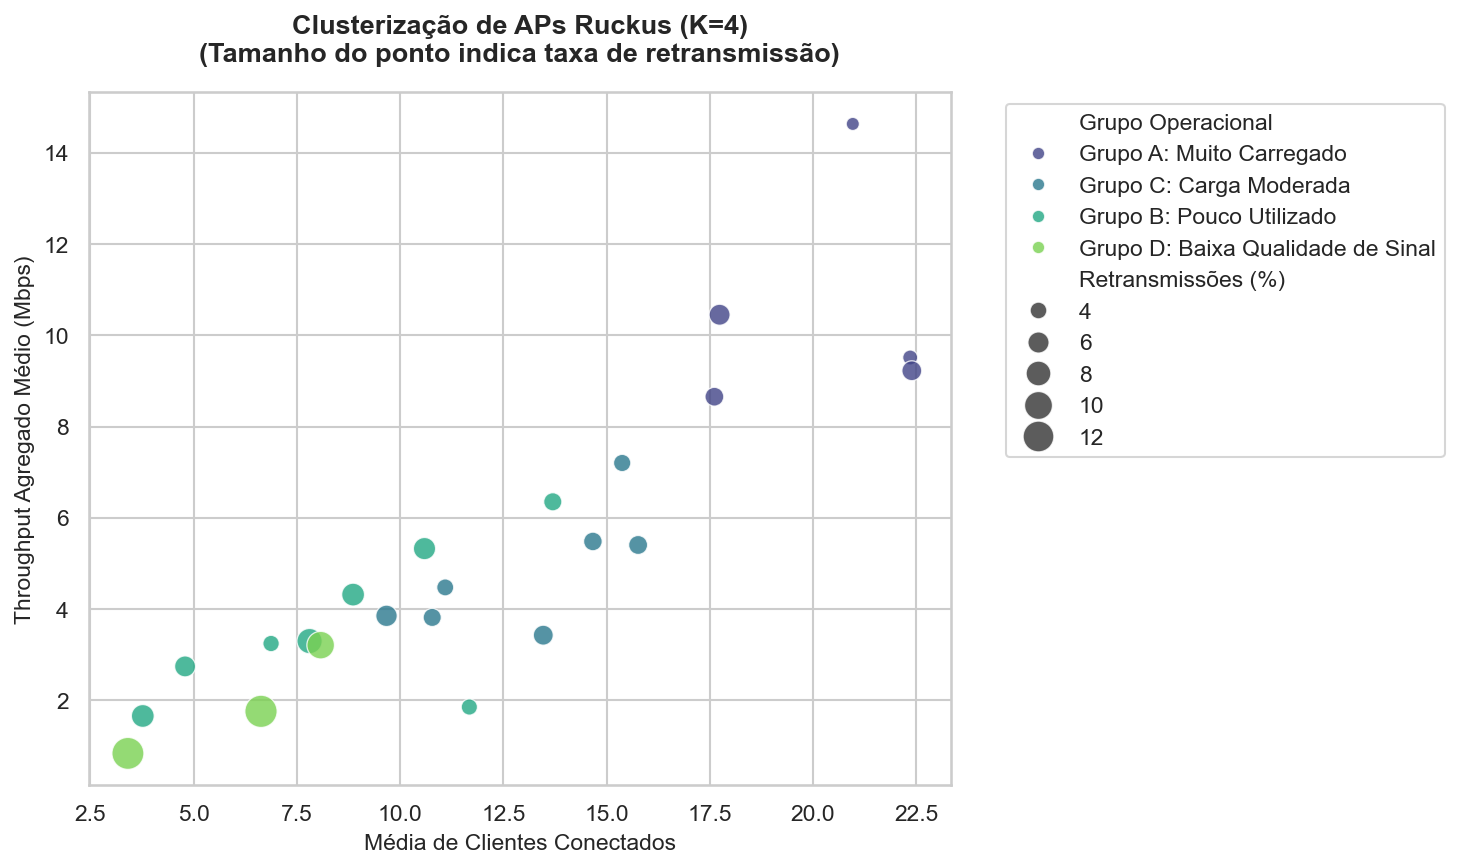
\includegraphics[width=0.85\textwidth]{img/cluster_ruckus.png}
  \caption{Clusterização Ruckus}
  \label{fig:cluster_ruckus_png}
\end{figure}

\begin{itemize}
  \item \textbf{UniFi}:
\end{itemize}
\begin{figure}[H]
  \centering
  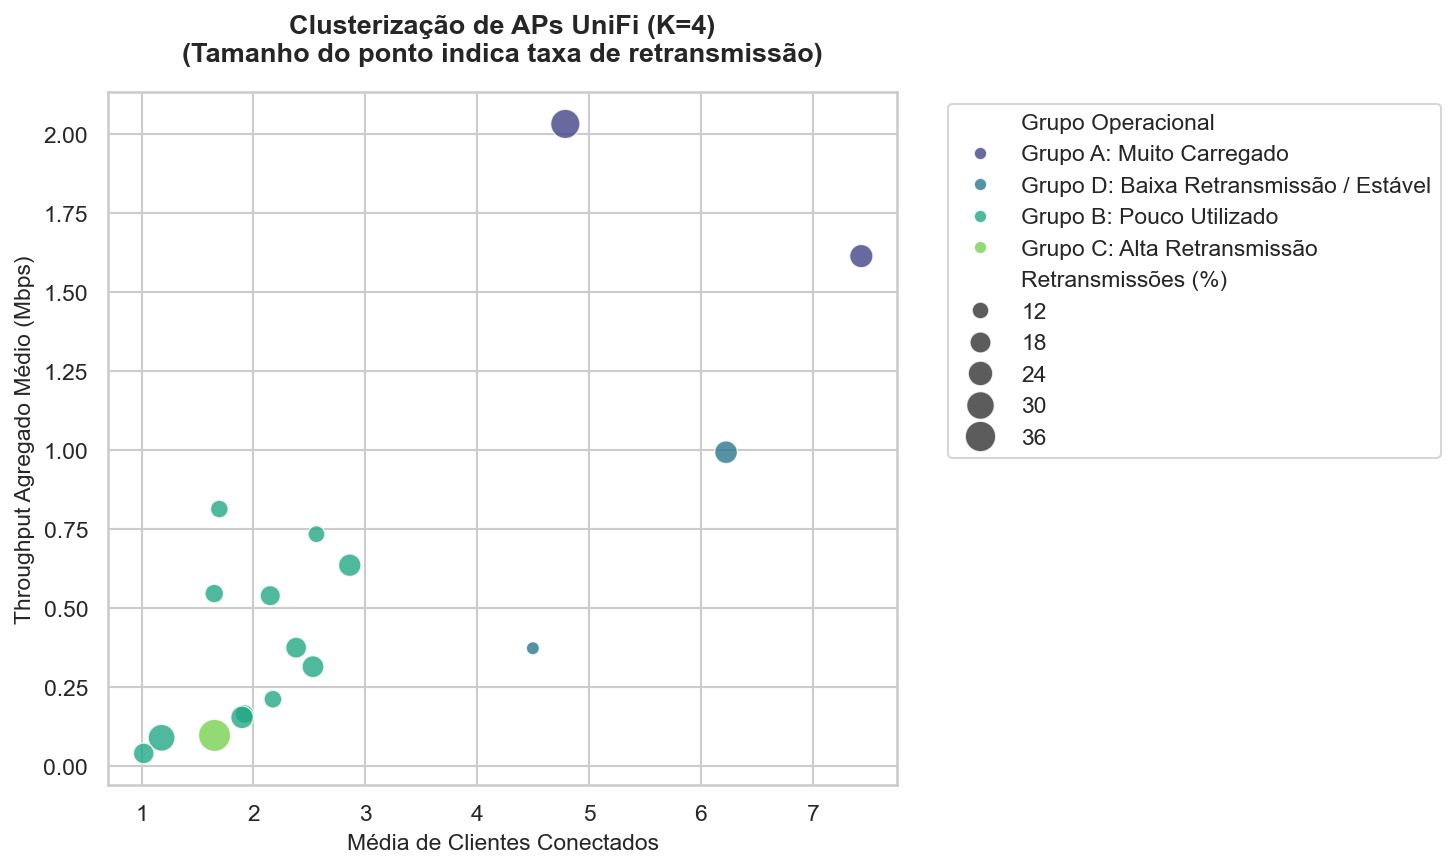
\includegraphics[width=0.85\textwidth]{img/cluster_unifi.png}
  \caption{Clusterização UniFi}
  \label{fig:cluster_unifi_png}
\end{figure}


